% Created 2023-04-14 Fri 08:42
\documentclass[9pt, b5paaper]{book}
\usepackage{xeCJK}
\usepackage[T1]{fontenc}
\usepackage[scaled]{beraserif}
\usepackage[scaled]{berasans}
\usepackage[scaled]{beramono}
\usepackage{graphicx}
\usepackage{xcolor}
\usepackage{multirow}
\usepackage{multicol}
\usepackage{float}
\usepackage{textcomp}
\usepackage{geometry}
\geometry{left=1.2cm,right=1.2cm,top=1.5cm,bottom=1.2cm}
\usepackage{algorithm}
\usepackage{algorithmic}
\usepackage{latexsym}
\usepackage{natbib}
\usepackage{minted}
\newminted{common-lisp}{fontsize=\footnotesize}
\usepackage[xetex,colorlinks=true,CJKbookmarks=true,linkcolor=blue,urlcolor=blue,menucolor=blue]{hyperref} 
\author{deepwaterooo}
\date{\today}
\title{dataStructure}
\hypersetup{
  pdfkeywords={},
  pdfsubject={},
  pdfcreator={Emacs 28.2 (Org mode 8.2.7c)}}
\begin{document}

\maketitle
\tableofcontents


\chapter{Segment Tree与Binary Index Tree 线段树与树状数组}
\label{sec-1}

线段树(segment tree),顾名思义, 是用来存放给定区间(segment, or interval)内对应信息的一种数据结构。与树状数组(binary indexed tree)相似,线段树也用来处理数组相应的区间查询(range query)和元素更新(update)操作。与树状数组不同的是,线段树不止可以适用于区间求和的查询,也可以进行区间最大值,区间最小值(Range Minimum/Maximum Query problem)或者区间异或值的查询。

对应于树状数组,线段树进行更新(update)的操作为O(logn),进行区间查询(range query)的操作也为O(logn)。

\subsection{1157. Online Majority Element In Subarray - Hard}
\label{sec-1-0-1}
Design a data structure that efficiently finds the majority element of a given subarray.

The majority element of a subarray is an element that occurs threshold times or more in the subarray.

Implementing the MajorityChecker class:

MajorityChecker(int[] arr) Initializes the instance of the class with the given array arr.
int query(int left, int right, int threshold) returns the element in the subarray arr[left\ldots{}right] that occurs at least threshold times, or -1 if no such element exists.
\begin{enumerate}
\item 解题思路与分析
\label{sec-1-0-1-1}
\begin{itemize}
\item \url{https://www.cnblogs.com/slowbirdoflsh/p/11381565.html} 思路比较清晰
\end{itemize}

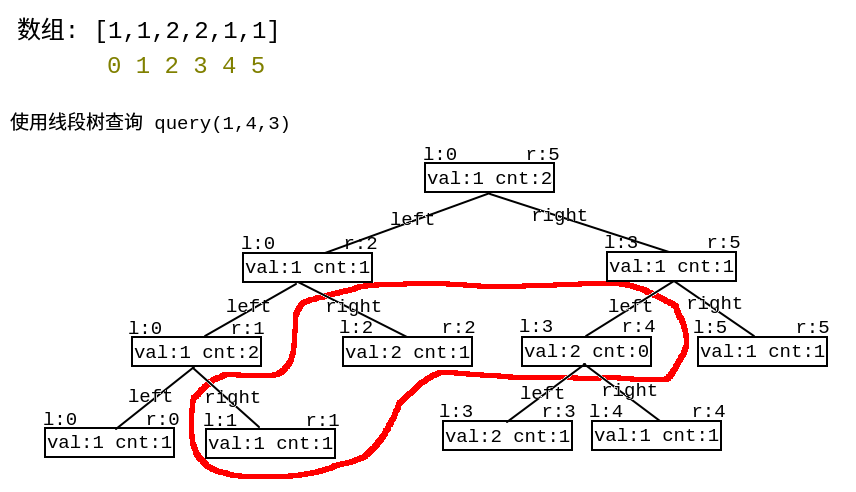
\includegraphics[width=.9\linewidth]{./pic/1157.png}

\begin{minted}[fontsize=\scriptsize,linenos=false]{csharp}
Map<Integer, List<Integer>> idx; // idx 存储数组出现元素种类 以及该元素下标索引
Node root; // 线段树的根节点
int key = 0, cnt = 0; // key 所查找的区域众数; count 所查找的区域众数出现次数, 
public MajorityChecker(int[] a) {
    idx = new HashMap<>(); // idx 存储数组出现元素种类 以及该元素下标索引
    for (int i = 0; i < a.length; i++)
        idx.computeIfAbsent(a[i], z -> new ArrayList<>()).add(i);
    root = buildTree(a, 0, a.length-1);
}
public int query(int left, int right, int threshold) {
    key = 0; cnt = 0; // 初始化 所查询众数key 及辅助判断的计数cnt
    searchTree(root, left, right); // 查询线段树
    // 如果查询区域没有众数 即key没被更改; 或者,
    // 所查询出来的众数 在原数组中根本没有超出阈值的能力
    if (key == 0 || idx.get(key).size() < threshold) return -1;
    // 上确界 排序数组中 第一个大于right的下标
    int r = upper_bound(idx.get(key), right);
    // 下确界 排序数组中 第一个大于等于left的下标
    int l = lower_bound(idx.get(key), left);
    cnt = r - l;
    return cnt >= threshold ? key : -1;
}
int upper_bound(List<Integer> list, int v) { // 排序数组中 第一个大于tar的下标
    int l = 0, r = list.size();
    while (l < r) {
        int mid = l + (r - l) / 2;
        if (list.get(mid) <= v) l = mid + 1;
        else r = mid;
    }
    return l;
}
int lower_bound(List<Integer> list, int v) { // 排序数组中 第一个大于等于tar的下标
    int l = 0, r = list.size();
    while (l < r) {
        int mid = l + (r - l) / 2;
        if (list.get(mid) < v) l = mid+1;
        else r = mid;
    }
    return l;
}
void searchTree(Node root, int l, int r) {
    if (root == null || l > r) return ;
    if (root.l > r || root.r < l) return ;
    if (root.l >= l && root.r <= r) { // 当查询边界被节点边界覆盖,该节点就是查询区域
        if (key == root.v) cnt += root.cnt;
        else if (cnt <= root.cnt) {
            key = root.v;
            cnt = root.cnt - cnt;
        } else cnt = cnt - root.cnt;
        return ;
    }
    int mid = (root.l + root.r) / 2; // 这两个查询条件再好好想想 !!!!!!!!!!!!!!!
    if (l <= mid)   // root.l <= l <= mid 左节点也可以是查询区域
        searchTree(root.left, l, r);
    if (r >= mid+1) // mid+1 <= r <= root.r 右节点也可以是查询区域
        searchTree(root.right, l, r);
}
Node buildTree(int [] a, int l, int r) {
    if (l > r) return null;
    Node root = new Node(l, r); // 初始一个线段树的根节点
    if (l == r) { // 叶子节点  
        root.v = a[l];
        root.cnt = 1;
        return root;
    }
    int mid = (l + r) / 2;
    root.left = buildTree(a, l, mid);
    root.right = buildTree(a, mid+1, r);
    makeRoot(root); // 整合父节点
    return root;
}
void makeRoot(Node r) { // 整合父节点
    if (r == null) return ;
    if (r.left != null) { // 如果该节点有左子节点 该节点的值"先"等于左子节点
        r.v = r.left.v;
        r.cnt = r.left.cnt;
    }
    if (r.right != null) { // 如果该节点还有右子节点 融合父节点和子节点
        if (r.v == r.right.v)
            r.cnt = r.cnt + r.right.cnt;
        else {
            if (r.cnt >= r.right.cnt)
                r.cnt = r.cnt - r.right.cnt;
            else {
                r.v = r.right.v;
                r.cnt = r.right.cnt - r.cnt;
            }
        }
    }
}
class Node {
    int l, r, v, cnt;
    Node left, right;
    public Node(int l, int r) {
        this.l = l; this.r = r;
        v = 0; cnt = 0;
        left = null; right = null;
    }
}
\end{minted}
\end{enumerate}

\subsection{1825. Finding MK Average - Hard}
\label{sec-1-0-2}
You are given two integers, m and k, and a stream of integers. You are tasked to implement a data structure that calculates the MKAverage for the stream.

The MKAverage can be calculated using these steps:

If the number of the elements in the stream is less than m you should consider the MKAverage to be -1. Otherwise, copy the last m elements of the stream to a separate container.
Remove the smallest k elements and the largest k elements from the container.
Calculate the average value for the rest of the elements rounded down to the nearest integer.
Implement the MKAverage class:

MKAverage(int m, int k) Initializes the MKAverage object with an empty stream and the two integers m and k.
void addElement(int num) Inserts a new element num into the stream.
int calculateMKAverage() Calculates and returns the MKAverage for the current stream rounded down to the nearest integer.
\begin{minted}[fontsize=\scriptsize,linenos=false]{csharp}
// 根据题意需要找到前k大的数,又需要求区间和,就自然想到线段树.写起来较不容易出错。
// 维护2个线段树数组,一个记录数的个数,一个记录区间值,
// 注意一般线段树中[s,e]指固定的区间,这里类似线段数求第k小的数,所以[s,e]指第s小的值到第e小的值的区间。
    Deque<Integer> q = new ArrayDeque<>(); // 始终维护m个数
    int [] cnt;  // 每个元素出现的次数
    long [] sum; // 累积和
    int m, k, n = 100000, N = n * 4 + 1; // 线段树所占用的空间为数组的四倍大小
    public MKAverage(int m, int k) {
        cnt = new int [N];
        sum = new long [N];
        this.m = m;
        this.k = k;
    }
    public void addElement(int num) {
        if (q.size() == m) {
            int v = q.pollFirst();
            insert(1, 0, n, v, -1); // 当删除掉一个元素的时候,需要更新线段树中的和
        }
        insert(1, 0, n, num, 1);
        q.offerLast(num);
    }
    public int calculateMKAverage() {
        if (q.size() < m) return -1;
        int bgn = k + 1, end = m - k; // idx: 1 - based
        return (int)(query(1, 0, n, bgn, end) / (m - 2 * k));
    }
    void insert(int idx, int l, int r, int v, long d) { // d: 
        cnt[idx] += d;
        sum[idx] += d * v;
        if (l == r) return ;
        int m = l + (r - l) / 2;
        if (v <= m)
            insert(idx << 1, l, m, v, d);       // 向左子树查询
        else insert(idx << 1 | 1, m+1, r, v, d);// 向右子树查询
    }
    long query(int idx, int l, int r, int bgn, int end) { // 线段中第 bgn 个到第 end 个
        if (l == r) { // 起始和结束最多出现2次此情况 ?
            int c = end - bgn + 1;
            return (long)c * l; //
        } else if (cnt[idx] == end - bgn + 1)
            return sum[idx];
        else {
            int m = l + (r - l) / 2;
            int cl = cnt[idx << 1];     // left child cnt
            // int cr = cnt[idx << 1 | 1];     // left child cnt
            if (cl >= end) // 搜索 左 子树
                return query(idx << 1, l, m, bgn, end); 
            else if (cl >= bgn) // 搜索 左 右 子树
                return query(idx << 1, l, m, bgn, cl) + query(idx << 1 | 1, m+1, r, 1, end - cl);
            else // cl < bgn, 搜索 右 子树
                return query(idx << 1 | 1, m+1, r, bgn - cl, end - cl);
        }
    }
\end{minted}
\begin{enumerate}
\item 解题思路与分析: 三个TreeMap, 自定义TreeMap
\label{sec-1-0-2-1}
\begin{minted}[fontsize=\scriptsize,linenos=false]{csharp}
    CusTreeMap [] ms;
    Deque<Integer> q;
    int m, k, n;
    public MKAverage(int m, int k) {
        this.m = m;
        this.k = k;
        q = new ArrayDeque<>();
        if (m - 2 * k > 0) {
            n = 3;
            ms = new CusTreeMap[n];
            ms[1] = new CusTreeMap(m - 2 * k);
        } else {
            n = 2;
            ms = new CusTreeMap[n];
        }
        ms[0] = new CusTreeMap(k);
        ms[n-1] = new CusTreeMap(k);
    }
    // 删除num,结果总是使mapList的小、中、大三个treemap依次填充。(先保证最小的treeMap填充、再保证中间的treeMap填充、最后是最大的填充)
    private void removeElement(int num) {
        boolean removed = false;
        for (int i = 0; i < n; i++) {
            if (!removed)
                removed = ms[i].remove(num);
            else { // 将后现一两个图中的最小元素向前一个图中挪动一个数值
                Integer minK = ms[i].pollFirst();
                if (minK == null) break;
                ms[i-1].add(minK);
            }
        }
    }
    public void addElement(int num) {
        if (q.size() == m) {
            int v = q.pollFirst();
            removeElement(v);
        }
        q.offerLast(num);
        Integer vtoAdd = num;
        for (int i = 0; i < n && vtoAdd != null; i++) 
            vtoAdd = ms[i].add(vtoAdd); // 记得这里返回的是: 如果图中已有k个元素,扔出来的最大键
    }
    public int calculateMKAverage() {
        if (q.size() < m || n < 3) return -1;
        return ms[1].avg();
    }
    class CusTreeMap {
        TreeMap<Integer, Integer> m;
        final int capacity;
        int size, sum;
        public CusTreeMap(int capacity) {
            m = new TreeMap<>();
            this.capacity = capacity;
        }
        public boolean remove(int key) {
            if (m.containsKey(key)) {
                m.put(key, m.get(key)-1);
                if (m.get(key) == 0) m.remove(key);
                sum -= key;
                size--;
                return true;
            }
            return false;
        }
        public Integer pollFirst() { // return key
            if (m.size() > 0) {
                int k = m.firstKey();
                // m.remove(k); // BUG: 你也不能用原始的TreeMap.remove(),因为它会移走所有的重复(如果这个元素存在重复的话)
                remove(k); // !!!
                return k;  // 这里没有自动更新 和 
                // return m.firstKey(); // BUG: 这里并没有真正移走这个元素,只是返回了第个元素的键
            }
            return null;
        }
        public Integer add(int key) { // 返回的是删除掉元素的键
            m.put(key, m.getOrDefault(key, 0) + 1); // 这里新填入的元素是否是最后一个元素,关系不大
            size++;
            sum += key;
            if (size > capacity) {
                int last = m.lastKey();
                m.put(last, m.get(last)-1);
                if (m.get(last) == 0) m.remove(last);
                sum -= last;
                size--;
                return last;
            }
            return null;
        }
        public int avg() {
            return sum / size;
        }
    }
\end{minted}
\item 解题思路与分析: 树状数组
\label{sec-1-0-2-2}
\begin{itemize}
\item 数状数组的解法: 另外第一次看到别人 二分+树状数组也能求前k大的值。
\end{itemize}
\begin{minted}[fontsize=\scriptsize,linenos=false]{csharp}
// We can have a queue to maintain m elements
// Use two Fenwick tree, 1 for count and 1 for prefix sum
// Do 2 times binary search for the first k elements and the last k elements by using the count from our first fenwick tree
// We can get the sum by subtrating the sum of first k elements and sum of last k element by using our second fenwick tree
Queue<Integer> q = new LinkedList<>();
FenWick fone, ftwo;
int [] cnt = new int [100010];
long sum = 0;
int m,k;
public MKAverage(int m, int k) {
    this.m = m;
    this.k = k;
    long A [] = new long [100010];
    long B [] = new long [100010];
    fone = new FenWick(A);
    ftwo = new FenWick(B);
}
public void addElement(int num) {
    q.add(num);
    sum += num;
    fone.update(num, 1);
    ftwo.update(num, num);
    cnt[num]++;
}
public int calculateMKAverage() {
    if (q.size() < m) return -1;
    while (q.size() > m) {
        int cur = q.poll();
        cnt[cur]--;
        sum -= cur;
        fone.update(cur, -1);
        ftwo.update(cur, -cur);
    }
    // binary search for the first k (there may be duplicated)
    int l = 0, r = cnt.length-1;
    int i = -1, j = -1; // pos1, pos2 
    while (l <= r) { // 二分查找总计数
        int m = (r + l) / 2;
        long count = fone.sumRange(0, m);
        if (count >= k) {
            i = m;
            r = m -1;
        } else l = m+1;
    }
    // binary search for the last k (there may be duplicated)
    l = 0;
    r = cnt.length-1;
    while (l <= r) {
        int m = l + (r-l)/2;
        long count = fone.sumRange(m, cnt.length-1);
        if (count >= k) {
            j = m;
            l = m + 1;
        } else r = m-1;
    }
    long sum1 = ftwo.sumRange(0,  i);
    long sum2 = ftwo.sumRange(j, cnt.length-1);
    long cnt1 = fone.sumRange(0, i);
    long cnt2 = fone.sumRange(j, cnt.length-1);
    if (cnt1 > k)
        sum1 -= i*(cnt1-k);
    if (cnt2 > k)
        sum2 -= j*(cnt2-k);
    long remain = sum - sum1 - sum2; // 总和, 减去两边最小最大各K个数的和
    return (int)(remain / (m-2*k));
}
class FenWick {
    long tree []; //1-index based
    long A [];
    long arr[];
    public FenWick(long [] A) {
        this.A = A;
        arr = new long [A.length];
        tree = new long [A.length + 1];
    }
    public void update(int i, int v) {
        arr[i] += v;
        i++;
        while (i < tree.length) {
            tree[i] += v;
            i += (i & -i); // 这是的原理细节再回去复习一下
        }
    }
    public long sumRange(int i, int j) {
        return pre(j+1)-pre(i);
    }
    public long pre(int i) {
        long sum = 0;
        while (i > 0) {
            sum += tree[i];
            i -= (i & -i);
        }
        return sum;
    }
}
\end{minted}
\begin{itemize}
\item 其它比较有兴趣以的BST二叉树的解法,改天补起来
\end{itemize}
\end{enumerate}
\subsection{315. Count of Smaller Numbers After Self - Hard}
\label{sec-1-0-3}
You are given an integer array nums and you have to return a new counts array. The counts array has the property where counts[i] is the number of smaller elements to the right of nums[i].
\begin{enumerate}
\item 解题思路与分析: 二分查找的插入排序
\label{sec-1-0-3-1}
\begin{minted}[fontsize=\scriptsize,linenos=false]{csharp}
public List<Integer> countSmaller(int[] a) { // O(NlogN) 插入排序
    int n = a.length;
    List<Integer> ans = new ArrayList<>();
    List<Integer> list = new ArrayList<>(); // 新建一个list,用于排序
    int [] tmp = new int [n]; // 为了提高效率,新建一个数组型的返回结果
    for (int i = n-1; i >= 0; i--) {
        int v = a[i];       // 将当前数字插入到新建list中, 使用二分查找找到插入位置
        int l = 0, r = list.size()-1; // l: left; r: right 从排好序的list中二分查找正确的插入位置
        while (l <= r) {
            int m = l + (r - l) / 2;
            if (v <= list.get(m)) r = m-1;
            else l = m + 1;
         }
        list.add(l, v); // 将当前数字插入到相应位置,保证list升序排列
        tmp[i] = l; // 当前位置前所有数字均小于当前数字,将个数加入返回结果
    }
    for (Integer v : tmp) ans.add(v);
    return ans;
}
\end{minted}
\item 解题思路与分析: 数状数组
\label{sec-1-0-3-2}
\begin{itemize}
\item 官方题解: \url{https://leetcode-cn.com/problems/count-of-smaller-numbers-after-self/solution/ji-suan-you-ce-xiao-yu-dang-qian-yuan-su-de-ge-s-7/}
\begin{minted}[fontsize=\scriptsize,linenos=false]{csharp}
private int[] c;
private int[] a; // 离散化、去重复 后的数组
public List<Integer> countSmaller(int[] nums) {
    List<Integer> ans = new ArrayList<Integer>(); 
    discretization(nums);
    init(nums.length + 5);
    for (int i = nums.length - 1; i >= 0; --i) {
        int id = getId(nums[i]);
        ans.add(query(id - 1));
        update(id);
    }
    Collections.reverse(ans);
    return ans;
}
private void init(int length) {
    c = new int[length];
    Arrays.fill(c, 0);
}
private int lowBit(int x) {
    return x & (-x);
}
private void update(int pos) {
    while (pos < c.length) {
        c[pos] += 1;
        pos += lowBit(pos);
    }
}
private int query(int pos) {
    int ret = 0;
    while (pos > 0) {
        ret += c[pos];
        pos -= lowBit(pos);
    }
    return ret;
}
private void discretization(int[] nums) { // 离散化、去重复 ?
    Set<Integer> set = new HashSet<Integer>(Arrays.stream(nums).boxed().collect(Collectors.toList()));
    int size = set.size();
    a = new int[size];
    int index = 0;
    for (int num : set) a[index++] = num;
    Arrays.sort(a);
}
private int getId(int x) {
    return Arrays.binarySearch(a, x) + 1; // 
}
\end{minted}
\end{itemize}
\item 解题思路与分析: 归并排序 todo 补上
\label{sec-1-0-3-3}
\end{enumerate}

\subsection{327. Count of Range Sum - Hard \textbf{重点} 这几个题要好好再理解消化几遍}
\label{sec-1-0-4}
Given an integer array nums and two integers lower and upper, return the number of range sums that lie in [lower, upper] inclusive.

Range sum S(i, j) is defined as the sum of the elements in nums between indices i and j inclusive, where i <= j.
\begin{enumerate}
\item 解题思路与分析: 分治法
\label{sec-1-0-4-1}

在累积和的基础上,我们计算有多少个区间的大小落在[lower, upper]之间,一个朴素的算法就是枚举各个区间,其时间复杂度是O(n\^{}2)。一个更好的方法是利用分治法来处理,即利用归并排序算法将数组分成左右两边,在合并左右数组之前,对于左边数组中的每一个元素,在右边数组找到一个范围,使得在这个范围中的元素与左边元素构成的区间和落在[lower, upper]之间,即在右边数组中找到两个边界,设为m,n,其中m是在右边数组中第一个使得sum[m] - sum[i] >= lower的位置,而n是第一个使得sum[n] - sum[i] > upper的位置,这样n-m就是与左边元素i所构成的位于[lower, upper]范围的区间个数。因为左右两边都是已经有序的,这样就可以避免不必要的比较(这也是为什么我们能将时间复杂度从O(n\^{}2)降低到O(nlogn)的秘诀所在)。

\begin{minted}[fontsize=\scriptsize,linenos=false]{csharp}
public int countRangeSum(int[] a, int lower, int upper) { // 这个merge sort的思维很奇特: 二分,O(NlogN)
    int n = a.length;
    long [] sum = new long[n+1];
    for (int i = 1; i <= n; i++) 
        sum[i] = sum[i-1] + a[i-1];
    return mergeAnalyse(sum, 0, n+1, lower, upper);
}
int mergeAnalyse(long [] a, int l, int r, int lo, int hi) { // l, r: 寻找[l, r)范围内和为[lower, upper]的片段的个数
    if (r - l <= 1) return 0;
    int mid = l + (r - l) / 2;
    int m = mid, n = mid, ans = 0;
    ans = mergeAnalyse(a, l, mid, lo, hi) + mergeAnalyse(a, mid, r, lo, hi);
    for (int i = l; i < mid; i++) { // 遍历[l, r)的半段长度: pivot 右移,滑动窗口,寻找合法窗口 // 通过遍历寻找当前范围中符合要求的个数,
        while (m < r && a[m] - a[i] < lo) m++; // 左端点右移,直到找到合法(sum >= lo)的解:m合法
        while (n < r && a[n] - a[i] <= hi) n++; // 右端点右移,直到右端点右移至不再合法(sum > hi), n 不合法 
        ans += n - m; // 对于[l, r)范围内的当前i来说,满足要求的总个数为 n - m
    }
    Arrays.sort(a, l, r); // 将[l, r)片段排序
    return ans;
}
\end{minted}
\item 解题思路与分析: 线段树
\label{sec-1-0-4-2}
\begin{itemize}
\item 官方题解:\url{https://leetcode-cn.com/problems/count-of-range-sum/solution/qu-jian-he-de-ge-shu-by-leetcode-solution/} 
\begin{minted}[fontsize=\scriptsize,linenos=false]{csharp}
public int countRangeSum(int[] a, int lo, int hi) {
    int n = a.length;
    long [] preSum = new long[n + 1];
    for (int i = 1; i <= n; i++) 
        preSum[i] = preSum[i-1] + a[i-1];
    Set<Long> allNumbers = new TreeSet<Long>();
    for (long x : preSum) {
        allNumbers.add(x);
        allNumbers.add(x - lo); //
        allNumbers.add(x - hi); // 
    }
    // 利用哈希表进行离散化
    Map<Long, Integer> values = new HashMap<Long, Integer>();
    int idx = 0;
    for (long x : allNumbers) {
        values.put(x, idx);
        idx++;
    }
    SegNode root = build(0, values.size() - 1);
    int ret = 0;
    for (long x : preSum) {
        int left = values.get(x - hi), right = values.get(x - lo);
        ret += count(root, left, right);
        insert(root, values.get(x));
    }
    return ret;
}
public SegNode build(int left, int right) {
    SegNode node = new SegNode(left, right);
    if (left == right) {
        return node;
    }
    int mid = (left + right) / 2;
    node.lchild = build(left, mid);
    node.rchild = build(mid + 1, right);
    return node;
}
public int count(SegNode root, int left, int right) {
    if (left > root.hi || right < root.lo) 
        return 0;
    if (left <= root.lo && root.hi <= right) 
        return root.add;
    return count(root.lchild, left, right) + count(root.rchild, left, right);
}
public void insert(SegNode root, int val) {
    root.add++;
    if (root.lo == root.hi) 
        return;
    int mid = (root.lo + root.hi) / 2;
    if (val <= mid) 
        insert(root.lchild, val);
    else insert(root.rchild, val);
}
class SegNode {
    int lo, hi, add;
    SegNode lchild, rchild;
    public SegNode(int left, int right) {
        lo = left;
        hi = right;
        add = 0;
        lchild = null;
        rchild = null;
    }
}
\end{minted}
\end{itemize}
\item 解题思路与分析: 动态增加节点的线段树 todo
\label{sec-1-0-4-3}
\item 解题思路与分析: 树状数组
\label{sec-1-0-4-4}
\begin{minted}[fontsize=\scriptsize,linenos=false]{csharp}
public int countRangeSum(int[] a, int lower, int upper) { // 树状数组
    int n = a.length;
    long[] preSum = new long[a.length + 1];
    for (int i = 1; i <= n; i++) 
        preSum[i] = preSum[i-1] + a[i-1];
    Set<Long> allNumbers = new TreeSet<Long>();
    for (long x : preSum) {
        allNumbers.add(x);
        allNumbers.add(x - lower);
        allNumbers.add(x - upper);
    }
    // 利用哈希表进行离散化
    Map<Long, Integer> values = new HashMap<Long, Integer>();
    int idx = 0;
    for (long x: allNumbers) {
        values.put(x, idx);
        idx++;
    }
    int ret = 0;
    BIT bit = new BIT(values.size());
    for (int i = 0; i < preSum.length; i++) {
        int left = values.get(preSum[i] - upper), right = values.get(preSum[i] - lower);
        ret += bit.query(right + 1) - bit.query(left);
        bit.update(values.get(preSum[i]) + 1, 1);
    }
    return ret;
}
class BIT {
    int [] tree;
    int n;
    public BIT(int n) {
        this.n = n;
        this.tree = new int[n + 1];
    }
    public int lowbit(int x) {
        return x & (-x);
    }
    public void update(int x, int d) {
        while (x <= n) {
            tree[x] += d;
            x += lowbit(x);
        }
    }
    public int query(int x) {
        int ans = 0;
        while (x != 0) {
            ans += tree[x];
            x -= lowbit(x);
        }
        return ans;
    }
}
\end{minted}
\item 解题思路与分析: 平衡二叉搜索树
\label{sec-1-0-4-5}
思路与算法

考虑一棵平衡二叉搜索树。若其节点数量为 NN,则深度为 O($\log$ N)O(logN)。二叉搜索树能够在 O($\log$ N)O(logN) 的时间内,对任意给定的值 val\}val,查询树中所有小于或等于该值的数量。

因此,我们可以从左到右扫描前缀和数组。对于 preSum\}[j]preSum[j] 而言,首先进行两次查询,得到区间 [preSum\}[j]-upper\}, preSum\}[j]-lower\}][preSum[j]−upper,preSum[j]−lower] 内的整数数量;随后再将 preSum[j] 插入到平衡树中。

平衡二叉搜索树有多种不同的实现,最经典的为 AVL 树与红黑树。此外,在算法竞赛中,还包括 Treap、SBT 等数据结构。

下面给出基于 Treap 的实现。

\begin{minted}[fontsize=\scriptsize,linenos=false]{csharp}
public int countRangeSum(int[] nums, int lower, int upper) {
    long sum = 0;
    long[] preSum = new long[nums.length + 1];
    for (int i = 0; i < nums.length; ++i) {
        sum += nums[i];
        preSum[i + 1] = sum;
    }
    BalancedTree treap = new BalancedTree();
    int ret = 0;
    for (long x : preSum) {
        long numLeft = treap.lowerBound(x - upper);
        int rankLeft = (numLeft == Long.MAX_VALUE ? (int) (treap.getSize() + 1) : treap.rank(numLeft)[0]);
        long numRight = treap.upperBound(x - lower);
        int rankRight = (numRight == Long.MAX_VALUE ? (int) treap.getSize() : treap.rank(numRight)[0] - 1);
        ret += rankRight - rankLeft + 1;
        treap.insert(x);
    }
    return ret;
}
class BalancedTree {
    private class BalancedNode {
        long val;
        long seed;
        int count;
        int size;
        BalancedNode left;
        BalancedNode right;
        BalancedNode(long val, long seed) {
            this.val = val;
            this.seed = seed;
            this.count = 1;
            this.size = 1;
            this.left = null;
            this.right = null;
        }
        BalancedNode leftRotate() {
            int prevSize = size;
            int currSize = (left != null ? left.size : 0) + (right.left != null ? right.left.size : 0) + count;
            BalancedNode root = right;
            right = root.left;
            root.left = this;
            root.size = prevSize;
            size = currSize;
            return root;
        }
        BalancedNode rightRotate() {
            int prevSize = size;
            int currSize = (right != null ? right.size : 0) + (left.right != null ? left.right.size : 0) + count;
            BalancedNode root = left;
            left = root.right;
            root.right = this;
            root.size = prevSize;
            size = currSize;
            return root;
        }
    }
    private BalancedNode root;
    private int size;
    private Random rand;
    public BalancedTree() {
        this.root = null;
        this.size = 0;
        this.rand = new Random();
    }
    public long getSize() {
        return size;
    }
    public void insert(long x) {
        ++size;
        root = insert(root, x);
    }
    public long lowerBound(long x) {
        BalancedNode node = root;
        long ans = Long.MAX_VALUE;
        while (node != null) {
            if (x == node.val) return x;
            if (x < node.val) {
                ans = node.val;
                node = node.left;
            } else node = node.right;
        }
        return ans;
    }
    public long upperBound(long x) {
        BalancedNode node = root;
        long ans = Long.MAX_VALUE;
        while (node != null) {
            if (x < node.val) {
                ans = node.val;
                node = node.left;
            } else node = node.right;
        }
        return ans;
    }
    public int[] rank(long x) {
        BalancedNode node = root;
        int ans = 0;
        while (node != null) {
            if (x < node.val) {
                node = node.left;
            } else {
                ans += (node.left != null ? node.left.size : 0) + node.count;
                if (x == node.val) {
                    return new int[]{ans - node.count + 1, ans};
                }
                node = node.right;
            }
        }
        return new int[]{Integer.MIN_VALUE, Integer.MAX_VALUE};
    }
    private BalancedNode insert(BalancedNode node, long x) {
        if (node == null) 
            return new BalancedNode(x, rand.nextInt());
        ++node.size;
        if (x < node.val) {
            node.left = insert(node.left, x);
            if (node.left.seed > node.seed) 
                node = node.rightRotate();
        } else if (x > node.val) {
            node.right = insert(node.right, x);
            if (node.right.seed > node.seed) 
                node = node.leftRotate();
        } else ++node.count;
        return node;
    }
}
\end{minted}
\end{enumerate}
\subsection{699. Falling Squares - Hard}
\label{sec-1-0-5}
There are several squares being dropped onto the X-axis of a 2D plane.

You are given a 2D integer array positions where positions[i] = [lefti, sideLengthi] represents the ith square with a side length of sideLengthi that is dropped with its left edge aligned with X-coordinate lefti.

Each square is dropped one at a time from a height above any landed squares. It then falls downward (negative Y direction) until it either lands on the top side of another square or on the X-axis. A square brushing the left/right side of another square does not count as landing on it. Once it lands, it freezes in place and cannot be moved.

After each square is dropped, you must record the height of the current tallest stack of squares.

Return an integer array ans where ans[i] represents the height described above after dropping the ith square.
\begin{enumerate}
\item 解题思路与分析: O(N\^{}2) 本能土办法
\label{sec-1-0-5-1}
方块的大小不是固定的,有可能很大,但是不管方块再大,只要有一点点部分搭在其他方块上面,整个方块都会在上面,并不会掉下来,让我们求每落下一个方块后的最大高度。我们知道返回的是每落下一个方块后当前场景中的最大高度,那么返回的数组的长度就应该和落下方块的个数相同。所以我们可以建立一个heights数组,其中heights[i]表示第i块方块落下后所在的高度,那么第i块方块落下后场景的最大高度就是[0, i]区间内的最大值。那么我们在求出heights数组后,只要不停返回[0, i]区间内的最大值即可。继续来看,这道题的难点就是方块重叠的情况,我们先来想,如果各个方块不重叠,那么heights[i]的高度就是每个方块自身的高度。一旦重叠了,就得在已有的基础上再加上自身的高度。那么我们可以采用brute force的思想,对于每个一个下落的方块,我们都去看和后面将要落下的方块有没有重叠,有的话,和后面将要落下的方块的位置相比较,取二者中较大值为后面要落下的方块位置高度heights[j]。判读两个方块是否重叠的方法是如果方块2的左边界小于方块1的右边界,并且方块2点右边界大于方块1点左边界。就拿题目中的例子1来举例吧,第一个下落的方块的范围是[1, 3],长度为2,则heights\footnote{DEFINITION NOT FOUND.}=2,然后我们看其和第二个方块[2, 5]是否重叠,发现是重叠的,则heights\footnote{DEFINITION NOT FOUND.}更新为2,再看第三个方块[6, 7],不重叠,不更新。然后第二个方块落下,此时累加高度,则heights\footnotemark[2]{}=5,再看第三个方块,不重叠,不更新。然后第三个方块落下, heights\footnote{DEFINITION NOT FOUND.}=1。此时我们heights数组更新好了,然后我们开始从头遍历,维护一个当前最大值curMax,每次将[0, i]中最大值加入结果res即可,
\begin{minted}[fontsize=\scriptsize,linenos=false]{csharp}
public List<Integer> fallingSquares(int[][] a) {
    List<Integer> ans = new ArrayList<>();
    int n = a.length, max = 0;
    int [] hi = new int [n]; // 表示第 i 块方块落下后所在的高度
    for (int i = 0; i < n; i++) {
        int h = a[i][1], l = a[i][0], r = a[i][0] + h;
        hi[i] += h;
        for (int j = i+1; j < n; j++) {
            int ll = a[j][0], rr = ll + a[j][1];
            // [[6,1],[9,2],[2,4]] 因为不能保证是从左往下延x轴顺序掉落,所以加上l < rr 也狠重要 确保不管左右边有交叠
            if (ll < r && rr > l) // 保证j在i的右边,并且有重叠区域
                hi[j] = Math.max(hi[j], hi[i]);
        }
        max = Math.max(max, hi[i]);
        ans.add(max);
    }
    return ans;
}
\end{minted}
\item 解题思路与分析: 线段树 + 离散化
\label{sec-1-0-5-2}

想象x xx轴是地面,如果某个方块掉落的过程中遇到了之前的某个方块(擦边而过不算),则该方块会叠到上面。现在给定一个长n nn数组A AA,A [ i ] A[i]A[i]存了第i ii个掉落的方块的信息,其中A [ i ] [ 0 ] A[i]\footnotemark[1]{}A[i]\footnotemark[1]{}表示它的左下角的x xx坐标,A [ i ] [ 1 ] A[i]\footnotemark[2]{}A[i]\footnotemark[2]{}表示它的边长。要求返回一个长n nn数组B BB,使得B [ i ] B[i]B[i]表示在A [ i ] A[i]A[i]掉落之后,当前所有方块的最高点的y yy坐标。

思路是线段树 + 离散化。可以将x xx坐标离散化,这样可以节省存储空间(离散化的过程其实就是将一个数组d dd排序后去重,然后将每个数映射到它的下标。这样在线段树建树的时候,就只需维护[ 0 , l d − 1 ] [0,l\_d-1][0,l\_d−1]这个区间的信息就行了,这会极大减少线段树的空间消耗,也从而会减少要做的操作的时间消耗)。具体来说,给定一个将要下落的方块,比如该方块的左端点的x xx坐标和右端点的x xx坐标分别是a aa和b bb,边长是c cc,那么我们需要实现两个操作,第一是查询( a , b ) (a,b)(a,b)里的最大值M MM(注意这里查询的是开区间( a , b ) (a,b)(a,b)的最大值,因为下落的方块擦着另一个方块的边的话,是不会叠上去的),另一个是将[ a , b ] [a,b][a,b]里所有值都变成M + c M+cM+c。本质上是要求一个数据结构可以查询区间最大值,以及将区间修改为某一值,这可以用线段树 + 懒标记来做到。在离散化之后,为了使得区间( a , b ) (a,b)(a,b)非空(注意这里a aa和b bb都是离散化之后的值,此时( a , b ) = [ a + 1 , b − 1 ] (a,b)=[a+1,b-1](a,b)=[a+1,b−1]),我们可以在离散化的时候将方块的中点也加入一起做离散化,但是这会导致中点变成非整数,这里将原坐标乘以2 22就行了。

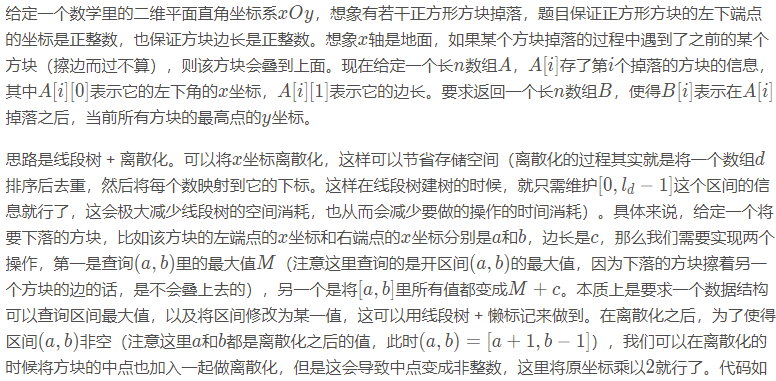
\includegraphics[width=.9\linewidth]{./pic/699.png}

\begin{minted}[fontsize=\scriptsize,linenos=false]{csharp}
public List<Integer> fallingSquares(int[][] a) { // 需要对数据进行离散化处理,离散化的目的是为了线段树处理起来方便;离散的是x轴的横坐标
    List<Integer> x = new ArrayList<>();
    for (int [] v : a) {
        int i = v[0], j = i + v[1];
        x.add(i * 2);
        x.add(j * 2);
        x.add(i + j);
    }
    x = getUniques(x);
    MaxSeg maxSeg = new MaxSeg(x.size());
    List<Integer> ans = new ArrayList<>();
    for (int [] v : a) {
        int i = v[0], j = i + v[1];
        i = getIdxInList(i * 2, x);
        j = getIdxInList(j * 2, x);
        int h = maxSeg.query(1, i+1, j-1);
        maxSeg.update(1, i, j, h + v[1]);
        ans.add(maxSeg.query());
    }
    return ans;
}
int getIdxInList(int v, List<Integer> list) { // 找到 x 在离散化之后的值是多少,其实就是求 xs 里 x 的下标,可以二分来找到
    int l = 0, r = list.size()-1;
    while (l < r) {
        int m = l + (r - l) / 2;
        if (list.get(m) >= v) r = m;
        else l = m + 1;
    }
    return l;
}
List<Integer> getUniques(List<Integer> l) {
    l.sort(Integer::compareTo);
    int j = 0; // 返回结果链表的下标 idx
    for (int i = 0; i < l.size(); i++) {
        if (i == 0 || l.get(j-1) != l.get(i))
            l.set(j++, l.get(i));
    }
    return l.subList(0, j);
}
class MaxSeg {   // 实现一下带懒标记的线段树 : 这棵树好强大
    class Node { // v 是 [l, r] 区间的最大值, lazy 是懒标记
        int l, r, v, lazy;
        public Node(int l, int r) {
            this.l = l;
            this.r = r;
        }
    }
    Node [] tree;
    public MaxSeg(int n) {
        tree = new Node[n << 2]; // n * 2 * 2
        buildTree(1, 0, n-1);    // 下标从 1 开始 自顶向下
    }
    void buildTree(int i, int l, int r) {
        tree[i] = new Node(l, r);
        if (l == r) return;
        int m = l + r >> 1; // (l + r) / 2
        buildTree(i << 1, l, m);
        buildTree(i << 1 | 1, m+1, r);
    }
    void pushUp(int i) { // 自底向上:自左、右叶子节点向顶更新最大值,取左右节点的最大值
        tree[i].v = Math.max(tree[i << 1].v, tree[i << 1 | 1].v);
    }
    void pushDown(int i) { // 懒标记向底、叶子方向推进一层
        int c = tree[i].lazy;
        if (c != 0) { // 打有懒标记
            tree[i].lazy = 0;
            tree[i << 1].v = tree[i << 1 | 1].v = c;
            tree[i << 1].lazy = tree[i << 1 | 1].lazy = c;
        }
    }
    void update(int i, int l, int r, int c) {   // 自顶向下传递懒标记,再自底向上更新父节点的值:取左右子节点的最大值
        if (l <= tree[i].l && tree[i].r <= r) { // 任务不需要下发,可以用懒标记懒住
            tree[i].v = tree[i].lazy = c; // 这里 tree[i].v = tree[i].lazy = c : c 是想要更新到的新值v, 用它来更新懒标记和v值
            return ;
        }
        pushDown(i);  // 任务不得不下发,则先下发给两个孩子
        int m = tree[i].l + tree[i].r >> 1;
        if (l <= m) update(i << 1, l, r, c);  // 回归调用,下传更新至左右子节点
        if (m + 1 <= r) update(i << 1 | 1, l, r, c);
        pushUp(i);  // 孩子完成了任务,再修改自己的值
    }
    int query(int i, int l, int r) {
        if (l <= tree[i].l && r >= tree[i].r) return tree[i].v;
        pushDown(i);
        int ans = 0, m = tree[i].l + tree[i].r >> 1;
        if (l <= m) ans = Math.max(ans, query(i << 1, l, r));
        if (m + 1 <= r) ans = Math.max(ans, query(i << 1 | 1, l, r));
        return ans;
    }
    int query() {
        return tree[1].v;
    }
}
\end{minted}
\item 解题思路与分析: 超简洁版的线段树,效率奇高
\label{sec-1-0-5-3}
\begin{itemize}
\item \url{http://www.noobyard.com/article/p-sxwzvpgp-nz.html}
\item 去找一下原文件中的优化步骤
\begin{minted}[fontsize=\scriptsize,linenos=false]{csharp}
private class Node { // 描述方块以及高度
    int l, r, h, maxR;
    Node left, right;
    public Node(int l, int r, int h, int maxR) {
        this.l = l;
        this.r = r;
        this.h = h;
        this.maxR = maxR;
        this.left = null;
        this.right = null;
    }
}
public List<Integer> fallingSquares(int[][] positions) {
    List<Integer> res = new ArrayList<>(); // 建立返回值
    Node root = null; // 根节点,默认为零
    int maxH = 0; // 目前最高的高度
    for (int[] position : positions) {
        int l = position[0]; // 左横坐标
        int r = position[0] + position[1]; // 右横坐标
        int e = position[1]; // 边长
        int curH = query(root, l, r); // 目前区间的最高的高度
        root = insert(root, l, r, curH + e);
        maxH = Math.max(maxH, curH + e);
        res.add(maxH);
    }
    return res;
}
private Node insert(Node root, int l, int r, int h) {
    if (root == null) return new Node(l, r, h, r);
    if (l <= root.l)
        root.left = insert(root.left, l, r, h);
    else
        root.right = insert(root.right, l, r, h);
    root.maxR = Math.max(r, root.maxR); // 最终目标是仅仅须要根节点更新 maxR
    return root; // 返回根节点
}
private int query(Node root, int l, int r) {
    // 新节点的左边界大于等于目前的maxR的话,直接获得0,不须要遍历了
    if (root == null || l >= root.maxR) return 0; 
    int curH = 0; // 高度
    if (!(r <= root.l || root.r <= l)) // 是否跟这个节点相交
        curH = root.h;
    // 剪枝
    curH = Math.max(curH, query(root.left, l, r));
    if (r > root.l)
        curH = Math.max(curH, query(root.right, l, r));
    return curH;
}
\end{minted}
\end{itemize}
\end{enumerate}
\subsection{1483. Kth Ancestor of a Tree Node - Hard 倍增法 binary lifting}
\label{sec-1-0-6}
You are given a tree with n nodes numbered from 0 to n - 1 in the form of a parent array parent where parent[i] is the parent of ith node. The root of the tree is node 0. Find the kth ancestor of a given node.

The kth ancestor of a tree node is the kth node in the path from that node to the root node.

Implement the TreeAncestor class:

TreeAncestor(int n, int[] parent) Initializes the object with the number of nodes in the tree and the parent array.
int getKthAncestor(int node, int k) return the kth ancestor of the given node node. If there is no such ancestor, return -1.
\begin{enumerate}
\item 解题思路与分析: 倍增 binary lifting
\label{sec-1-0-6-1}

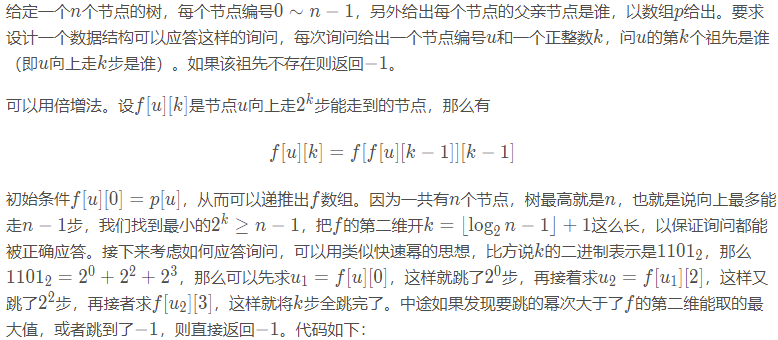
\includegraphics[width=.9\linewidth]{./pic/1483.png}

\begin{itemize}
\item 预处理时间复杂度O(nlogn),每次询问时间O(logn),空间O(nlogn)。

\begin{minted}[fontsize=\scriptsize,linenos=false]{csharp}
    private int [][] p;
    private int log;
    public TreeAncestor(int n, int[] parent) {
        log = (int) (Math.log(n - 1) / Math.log(2)) + 1;
        p = new int[n][log];
        for (int i = 0; i < parent.length; i++) // 初始化p数组
            p[i][0] = parent[i];
        for (int i = 1; i < log; i++) // 按公式递推p数组
            for (int j = 0; j < n; j++) 
                if (p[j][i-1] != -1) 
                    p[j][i] = p[p[j][i-1]][i-1];
                else p[j][i] = -1;
    }
    public int getKthAncestor(int node, int k) {
        int pow = 0;
        while (k > 0) {
            if (pow >= log || node == -1) return -1;
            if ((k & 1) == 1) 
                node = p[node][pow];
            k >>= 1;
            pow++;
        }
        return node;
    }
\end{minted}
\end{itemize}
\item 解题思路与分析
\label{sec-1-0-6-2}
\begin{minted}[fontsize=\scriptsize,linenos=false]{csharp}
    Map<Integer, List<Integer>> adj;
    int [][] par;
    public TreeAncestor(int n, int[] parent) {
        par = new int [n][30]; // 30 , 16: 不能证它是一棵很平衡的二叉树
        adj = new HashMap<>();
        for (int i = 0; i < n; i++) {
            Arrays.fill(par[i], -1);
            adj.put(i, new ArrayList<>());
        }
        for (int i = 0; i < parent.length; i++) 
            if (parent[i] != -1) {
                adj.get(parent[i]).add(i); // 自顶向下: 父 --》子节点
                par[i][0] = parent[i];     // 每个子节点的第一个父节点(2^0 = 1),即为父节点 // 自底向上: 子节点: 2^0父节点、 2^1节点、 2^2节点
            }
        dfs(0);
    }
    public int getKthAncestor(int node, int k) {
        for (int i = 0; k > 0; i++, k >>= 1) // k /= 2
            if ((k & 1) == 1) {
                node = par[node][i];
                if (node < 0) return -1;
            }
        return node;
    }
    private void dfs(int idx) { // 自顶向下:从父节点遍历子节点
        for (int i = 1; par[idx][i-1] >= 0; i++) // 穷追塑源:一直找到整棵树的根节点: 0
            par[idx][i] = par[par[idx][i-1]][i-1]; // 这里多想想
        for (int next : adj.get(idx)) 
            dfs(next);
    }
\end{minted}
\end{enumerate}
\subsection{236 二叉树的最近公共祖先}
\label{sec-1-0-7}

\subsection{1505. Minimum Possible Integer After at Most K Adjacent Swaps On Digits - Hard BIT树状数组}
\label{sec-1-0-8}
You are given a string num representing the digits of a very large integer and an integer k. You are allowed to swap any two adjacent digits of the integer at most k times.

Return the minimum integer you can obtain also as a string.
\begin{enumerate}
\item 解题思路与分析
\label{sec-1-0-8-1}
\begin{minted}[fontsize=\scriptsize,linenos=false]{csharp}
public String minInteger(String t, int k) {
    int n = t.length();
    t = " " + t;
    char [] s = t.toCharArray();
    ArrayDeque<Integer> [] q = new ArrayDeque [10];
    for (int i = 1; i <= n; i++) {
        int j = s[i] - '0';
        if (q[j] == null) q[j] = new ArrayDeque<>();
        q[j].offerLast(i);
    }
    BIT bit = new BIT(n);
    StringBuilder sb = new StringBuilder();
    for (int i = 1; i <= n; i++) {
        for (int j = 0; j < 10; j++) { // 从小数值往大数值遍历
            if (q[j] == null || q[j].isEmpty()) continue;
            int top = q[j].peekFirst(), pos = top + bit.sum(top); // pos是最优解的位置,最优解的位置是原来的位置加上偏移量
            if (pos - i <= k) {
                k -= pos - i;
                sb.append(j);
                q[j].pollFirst();
                bit.add(1, 1); // 更新[1, t)这段的值每个加1,即向右偏移1位.为什么要 从1开始更新:假装每次都移动到最前端,方便计算 ?
                bit.add(top, -1);
                break;
            }
        }
    }
    return sb.toString();
}
class BIT { // 开一个树状数组类,维护每个位置的字符的向右的偏移量 ? 向左偏移量
    private int n;
    private int [] a;
    public BIT(int n) {
        this.n = n;
        this.a = new int [n+1];
    }
    public void add(int idx, int v) { // 只有发生偏移,才移动某段区间的值
        while (idx <= n) {
            a[idx] += v;
            idx += lowbit(idx);
        }
    }
    public int sum(int idx) { // 得到以 i 为下标1-based的所有子、叶子节点的和, 也就是[1, idx]的和,1-based
        int ans = 0;
        while (idx > 0) {
            ans += a[idx];
            idx -= lowbit(idx);
        }
        return ans;
    }
    int lowbit(int x) {
        return x & -x;
    }
}
\end{minted}
\end{enumerate}

\chapter{Trie}
\label{sec-2}
应用
Trie树最直观的定义就是LinkedList of HashMap。所以Trie和HashMap都可以用来查询某个单词是否在字典当中。我们需要知道他们的优缺点。
优点:
支持字符级别的查询,比如说我们需要在matrix当中通过traverse构造单词,那么这个单词是一个一个字符形成的,我们可以在traverse的每一步去检验当前路径是否可以形成valid word。另外,对于含有regex符号的字符串,我们需要一个字符一个字符的考虑,这种情况下我们也需要通过trie去查找。
节省空间,相同的prefix只存一遍,而HashMap需要存很多遍。
缺点:实现起来较麻烦,大部分题目使用Trie都是overkill,所以除非需要支持字符级别的查询,否则HashMap更好。
操作: 三个操作:
insert
search
startWith
其中insert记得把最后一个node标记为isEnd = true。其中search和startWith都可以通过同一个searchHelper helper method来实现,我们只需要return 最后一个node就可以,如果isEnd == true,那么说明找到一个完整的单词,否则至少找到了prefix。别忘了使用trie的第一步是preprocess,把字典里的所有word加入到trie树当中。
题目
\section{208. Implement Trie (Prefix Tree)}
\label{sec-2-1}
\subsection{212. Word Search II}
\label{sec-2-1-1}
\subsection{211. Add and Search Word - Data structure design (Facebook店面)}
\label{sec-2-1-2}
\subsection{14. Longest Common Prefix (这道题可以稍作改编,比如说string list会经常update,会经常query,那这时很明显用trie更好)}
\label{sec-2-1-3}
\subsection{440. K-th Smallest in Lexicographical Order -  Hard}
\label{sec-2-1-4}
Given two integers n and k, return the kth lexicographically smallest integer in the range [1, n].
\begin{enumerate}
\item 解题思路与分析
\label{sec-2-1-4-1}
就像dfs时当我们需要两个字符串,遍历字符串,我们并不需要看的去遍历字符串,我们只要移动下标就可以了

这里我们并不需要真的去建和遍历这样一个字典,我们只要理清数字个数之间的关系就可以了

还要一个典型案例,把它找出来。。。。 todo

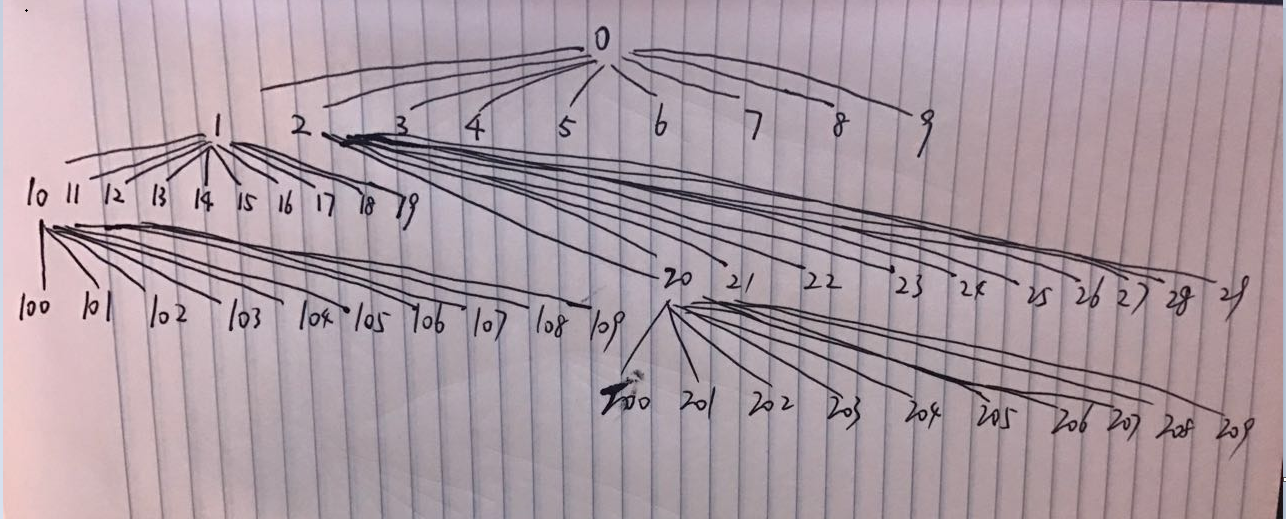
\includegraphics[width=.9\linewidth]{./pic/trie.png}

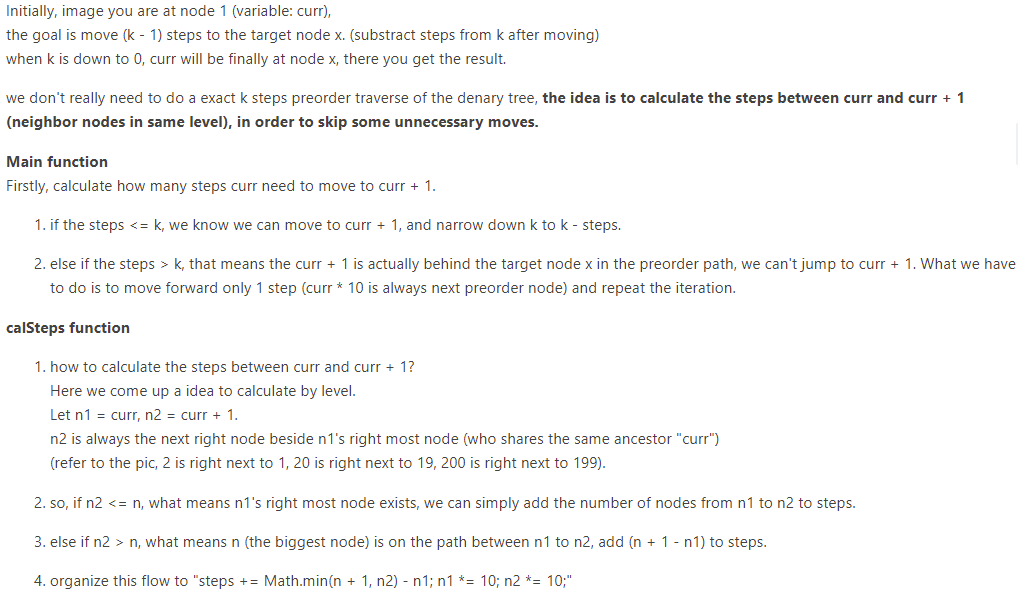
\includegraphics[width=.9\linewidth]{./pic/trie2.png}

\begin{minted}[fontsize=\scriptsize,linenos=false]{csharp}
private int calSteps(int n, long n1, long n2) { // n1 和 n2得是long类型的, int会产生溢出, 不能通过这个案例: 输入n=681692778, k=351251360, 预期结果=416126219
    int steps = 0;
    while (n1 <= n) {
        steps += Math.min(n2, n+1) - n1;
        n1 *= 10;
        n2 *= 10;
    }
    return steps;
}
public int findKthNumber(int n, int k) {
    int cur = 1; //根据题意, 第一个数是1
    --k;         //第一个是1, 所以再找出k-1个数后就知道第k个数是多少了
    while (k > 0) {
        int steps = calSteps(n, cur, cur+1);
        if (steps <= k) { //横向扩展, 相当于+steps,
            cur += 1;
            k -= steps;
        } else {          //steps > k; 纵向扩展, 相当于+1
            cur *= 10;
            k -= 1;
        }
    }
    return cur;
}
\end{minted}
\end{enumerate}

\subsection{421. Maximum XOR of Two Numbers in an Array}
\label{sec-2-1-5}
Given an integer array nums, return the maximum result of nums[i] XOR nums[j], where 0 <= i <= j < n.

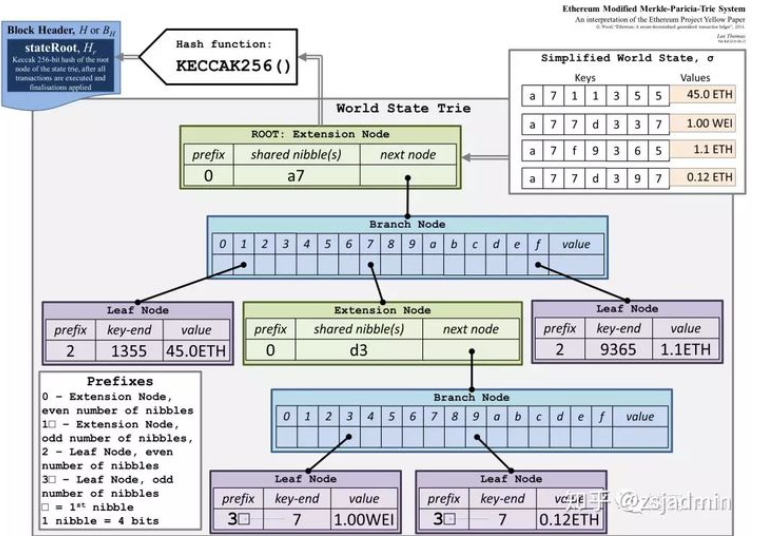
\includegraphics[width=.9\linewidth]{./pic/numTrie.png}

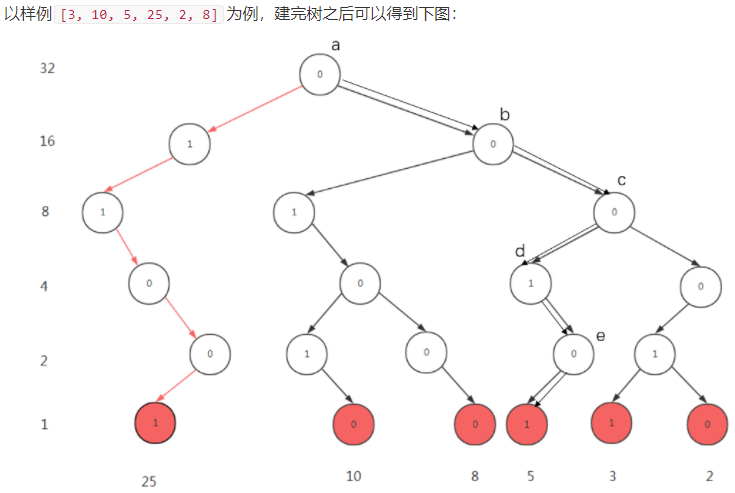
\includegraphics[width=.9\linewidth]{./pic/numTrie2.png}

左儿子为1的分支,右儿子为0的分支。

然后依次枚举每个数,在Trie树中找到与它异或结果最大的数。

这一步可以贪心来做:

从高位到低位,依次在Trie树中遍历,每次尽量走到与当前位不同的分支,这样可以使得找到的数与当前数在当前二进制位的异或结果是1,从而可以得到尽量大的结果。

如上图所示,我们用25来举例说明,它的二进制表示是(11001):

\begin{minted}[fontsize=\scriptsize,linenos=false]{csharp}
最初指针在根节点(编号是a的点),我们从25的二进制表示的最高位开始枚举;
  由于最高位是1,我们走到0分支,走到b点;
  次高位是1,我们继续往右儿子走,走到c点;
  下一位是0,我们往左走,走到d点;
  下一位是0,我们希望往左走,但发现左儿子不存在,所以只能往右走,走到e点;
  最后一位是1,我们希望往右走,但发现右儿子不存在,所以只能往左走,最终走到5;
所以和25异或值最大的数是5, 25 ^ 5 = 28。
\end{minted}
\begin{minted}[fontsize=\scriptsize,linenos=false]{csharp}
public class Trie {
    private class Node { // 这我自己写的乱代码,贴在这里很不相关,也需要先测试一下
        public int val;
        public boolean isExist;
        public Node [] next;
        public Node(boolean isExist) {
            this.isExist = isExist;
            next = new Node[2];
            val = 0;
        }
        public Node() { this(false); }
        public Node(int va) {
            this(true);
            this.val = va;
        }
    }
    private Node root;
    public Trie() { root = new Node(); }
    public void insert(int va) {
        Node cur = root;
        for (int i = 31; i >= 0; i--) {
            int tmp = (va >> i) & 1;
            if (cur.next[tmp] == null)
                cur.next[tmp] = new Node();
            cur = cur.next[tmp];
        }
        cur.isExist = true;
    }
    public int search(int va) {
        int max = 0;
        Node cur = root;
        for (int i = 31; i >= 0; i--) {
            int t = (va >> i) & 1;
            if (cur.next[t^1] != null) {
                max += (1 << i);
                cur = cur.next[t^1];
            } else cur = cur.next[t&1];
        }
        return max;
    }
}
\end{minted}

\begin{enumerate}
\item 另一种位操作法
\label{sec-2-1-5-1}

\begin{itemize}
\item 学到了异或操作的一个重要性质:a\^{}b = c, 则有 a\^{}c = b,且 b\^{}c = a;
\end{itemize}

我们还需要用上一个异或的特性,假设a和b产生了最终的答案max,即a \^{} b = x,那么根据异或的特性,a \^{} x = b。同理,a和b的最高位(前n位)也有相同的性质。

先以最高位为例子,我们可以把所有的数字的最高位放到一个HashSet里面,然后使用1与set里面的所有数字进行异或,如果得出的结果仍然在set里面,那么最终结果的最高位必然为1,否则为0。也即,先假定结果为1,然后与set中所有数字异或,假定a与1异或得到结果b(a \^{} 1 = b),而b仍然在set里面,那么说明set中有两个数字异或能得到1(a \^{} b = 1)。否则,set中没有两个数字能够异或得到1,那么最终结果的最高位为1的假设失败,说明最终结果的最高位为0。以此类推可以得到第二位、第三位。。。的数字。

再做一下推广,我们将所有数字的前N位放到一个HashSet里面,然后使用之前N-1位得到的最大值前缀prefix与set里面的所有数字进行异或,如果得出的结果仍然在set中,那么第N位必然为1,否则为0。

举个例子,给定数组[14, 11, 7, 2],二进制表示分别为[1110, 1011, 0111, 0010]。题目说了,数字最长不会超过32位,所以应从i = 31开始,但是所有数字中最多位4位数,简单起见,我直接从最高位i=3开始
\begin{minted}[fontsize=\scriptsize,linenos=false]{csharp}
[14,   11,   7,    2]
[1110, 1011, 0111, 0010]
1. i = 3, set = {1000, 0000} => max = 1000
2. i = 2, set = {1100, 1000, 0100, 0000} => max = 1100
3. i = 1, set = {1110, 1010, 0110, 0010} => max = 1100
4. i = 0, set = {1110, 1011, 0111, 0010} => max = 1100
\end{minted}
\begin{minted}[fontsize=\scriptsize,linenos=false]{csharp}
public int findMaximumXOR(int[] nums) { // 这种解法没有用到上面的这个trie呀
    int n = nums.length;
    int mask = 0, max = 0;
    HashSet<Integer> s = new HashSet<>();
    for (int i = 31; i >= 0; --i) { // i == 31时
        mask = mask | 1 << i;     // 为获取前n位的临时变量     
        for (int va : nums) 
            s.add(va & mask);     // 将所有数字的前n位放入set中
        int tmp = max | (1 << i); // 假定第n位为1,前n-1位max为之前迭代求得
        for (Integer va : s) 
            if (s.contains(va ^ tmp)) { // 查看`b`是否在 // i == 31, (va^tmp):  -2147483648
                max = tmp;              // b存在,第n位为1
                break;
            }
        s.clear();
    }
    return max;
}
// 此解法时间复杂度为O(32n)=O(n),空间复杂度上,我们使用了一个HashSet用于存储所有数字,因此空间复杂度是O(n)
\end{minted}
\end{enumerate}

\subsection{1617. Count Subtrees With Max Distance Between Cities - Hard}
\label{sec-2-1-6}
There are n cities numbered from 1 to n. You are given an array edges of size n-1, where edges[i] = [ui, vi] represents a bidirectional edge between cities ui and vi. There exists a unique path between each pair of cities. In other words, the cities form a tree.

A subtree is a subset of cities where every city is reachable from every other city in the subset, where the path between each pair passes through only the cities from the subset. Two subtrees are different if there is a city in one subtree that is not present in the other.

For each d from 1 to n-1, find the number of subtrees in which the maximum distance between any two cities in the subtree is equal to d.

Return an array of size n-1 where the dth element (1-indexed) is the number of subtrees in which the maximum distance between any two cities is equal to d.

Notice that the distance between the two cities is the number of edges in the path between them.
\begin{itemize}
\item So apparently the brute-force approach passed this question. I guess for future contests, I should really pay attention to the input size\ldots{}
\end{itemize}
\begin{enumerate}
\item 解题思路与分析:
\label{sec-2-1-6-1}

自己凭感觉写的,看别人的代码(尤其写得比较烦琐的前提下)不如自己的代码简炼

\begin{minted}[fontsize=\scriptsize,linenos=false]{csharp}
public int[] countSubgraphsForEachDiameter(int n, int[][] edges) { 
    int m = n-1, range = 1 << m, root = 0, cnt = 0;
    int [] ans = new int [m];
    for (int i = 1; i < range; i++) {
        root = -1;
        Map<Integer, List<Integer>> adj = new HashMap<>();
        for (int j = 0; j < m; j++)  // m edges
            if (((i >> j) & 1) == 1) {
                int [] e = edges[j];
                if (root == -1) root = e[0];
                adj.computeIfAbsent(e[0], z -> new ArrayList<>()).add(e[1]);
                adj.computeIfAbsent(e[1], z -> new ArrayList<>()).add(e[0]);
            }
        cnt = Integer.bitCount(i);
        Set<Integer> vis = new HashSet<>();
        max = 1;
        dfs(root, -1, adj, vis);
        if (vis.size() != cnt + 1) continue;
        ans[max-1]++;
    }
    return ans;
}
int max = 1;
private int dfs(int u, int p, Map<Integer, List<Integer>> m, Set<Integer> vis) { // 树的最大直径:
    vis.add(u);
    if (m.get(u).size() == 1 && m.get(u).get(0) == p) return 1; // 叶子节点 
    int fst = 0, sec = 0;
    for (Integer v : m.get(u)) {
        if (v == p) continue;
        int cur = dfs(v, u, m, vis);
        if (cur >= fst) {
            sec = fst;
            fst = cur;
        } else sec = Math.max(sec, cur);
    }
    max = Math.max(max, fst + sec); // bug: 这里 fst + sec 不需要 +1
    return fst + 1;
}
\end{minted}
\begin{itemize}
\item 另一种位操作法
\end{itemize}
\begin{minted}[fontsize=\scriptsize,linenos=false]{csharp}
One way in which we can find the diameter of a tree is using DFS, just like if our tree is represented using tree nodes instead of as grpah
    1. Make a call to DFS from any node as root, lets say 1 as root
    2. Maintain a global max parameter
    3. For each call to dfs, of all current nodes children (excluding parent)
       find top two distances from current node to any leaf reachable from current node
    4. Sum of these top two distances froms the longes path passing through current node to all its children. Update if this path is maximum
    5. return 1 + top distance for this dfs call. Need to add 1 since,
       max length of path that can be reached from current ndoe is current ndoe + max distance reachable from current ndoes's children
\end{minted}
\begin{minted}[fontsize=\scriptsize,linenos=false]{csharp}
public int [] countSubgraphsForEachDiameter(int n, int[][] edges) {
    ans = new int [n-1];
    for (int [] i : edges) { // if our node is 5, we store it as 1 << 4 which is 2^4
        graph.computeIfAbsent(1 << (i[0]-1), ArrayList::new).add(1 << (i[1]-1));
        graph.computeIfAbsent(1 << (i[1]-1), ArrayList::new).add(1 << (i[0]-1));
    }
    int range = (1 << n) - 1;  // (int)Math.pow(2, n) - 1;
    for (int subset = 3; subset <= range; subset++) {
        boolean isPowerOf2 = subset != 0 && (subset & (subset - 1)) == 0; // is power of 2
        if (isPowerOf2) continue;      // Single node subtrees can be excluded.
        max = 0; vis = 0;
        dfs(subset, Integer.highestOneBit(subset), -1); // Integer.highestOneBit(subset): subset: 0b1100, highest: 0b1000
        if (vis == subset)   // If visited is not equal to our current subset, all nodes are not reachable.
            ans[max - 1] ++; // In otherwords is not a proper subtree, hence dont include in the maxwer
    }
    return ans;
}
Map<Integer, List<Integer>> graph = new HashMap<>();
int max = 0, vis = 0;
int [] ans;
private int dfs(int subset, int cur, int pre) {
    if ((subset & cur) == 0) return 0; // 只遍历子集中存在的节点,换句话说,只遍历子集中存在的边,这样总图只建一遍就可以了
    vis = vis | cur; 
    int fstMax = 0, sndMax = 0;
    for (Integer next : graph.get(cur)) {
        if (next == pre) continue;
        int dist = dfs(subset, next, cur);
        if (dist > fstMax) {
            sndMax = fstMax;
            fstMax = dist;
        } else sndMax = Math.max(sndMax, dist);
    }
    max = Math.max(max, fstMax + sndMax); // top two distances from this node c
// top distance this cur node to any leaf is topdistance from c's children + 1. Adding 1 since we need to include cur node
    return 1 + fstMax;
}
\end{minted}
\begin{itemize}
\item 以前参考过的代码
\end{itemize}
\begin{minted}[fontsize=\scriptsize,linenos=false]{csharp}
public int [] countSubgraphsForEachDiameter(int n, int[][] edges) {
    int [] res = new int [n-1];
    List<List<int []>> subsets = new ArrayList<>();
    generateSubsets(edges, new ArrayList<int []>(), subsets, 0);
    for (List<int []> subset : subsets) 
        solve(subset, res);
    return res;
}
private void solve(List<int []> subset, int [] res) {
    if (!isValidGraph(subset)) return;
    Map<Integer, List<Integer>> graph = new HashMap<>();
    for (int [] eg : subset) {
        graph.computeIfAbsent(eg[0], k -> new ArrayList<>()).add(eg[1]);
        graph.computeIfAbsent(eg[1], k -> new ArrayList<>()).add(eg[0]);
    }
    int max = 1;
    for (Integer key : graph.keySet()) {
        if (graph.get(key).size() == 1) {
            int [] longest = new int [] {1}; // 减少global变量的数量
            Set<Integer> vis = new HashSet<>();
            vis.add(key);
            dfs(graph, vis, key, longest, 0);
            max = Math.max(max, longest[0]);
        }
    }
    res[max - 1]++;
}
private void dfs(Map<Integer, List<Integer>> graph, Set<Integer> vis, int idx, int [] longest, int level) {
    longest[0] = Math.max(longest[0], level);
    for (Integer node : graph.get(idx)) 
        if (vis.add(node)) // Set.add(element) return false if it contains element already
            dfs(graph, vis, node, longest, level + 1);
}
private boolean isValidGraph(List<int []> subset) {
    Set<Integer> nodes = new HashSet<>();
    for (int [] cur : subset) {
        nodes.add(cur[0]);
        nodes.add(cur[1]);
    }
    return nodes.size() - 1 <= subset.size();
}
private void generateSubsets(int [][] arr, List<int []> cur, List<List<int []>> res, int idx) {
    if (idx == arr.length) return; // arr.length <= 15, 用回塑法直接生成subsets,但是这是相对耗时的操作
    for (int i = idx; i < arr.length; i++) {
        cur.add(arr[i]);
        res.add(new ArrayList<>(cur));
        generateSubsets(arr, cur, res, i+1);
        cur.remove(cur.size()-1);
    }
}
\end{minted}
\end{enumerate}

\subsection{1938. Maximum Genetic Difference Query - Hard 离线算法、离线思维、批量处理、顺序无关}
\label{sec-2-1-7}
There is a rooted tree consisting of n nodes numbered 0 to n - 1. Each node's number denotes its unique genetic value (i.e. the genetic value of node x is x). The genetic difference between two genetic values is defined as the bitwise-XOR of their values. You are given the integer array parents, where parents[i] is the parent for node i. If node x is the root of the tree, then parents[x] == -1.

You are also given the array queries where queries[i] = [nodei, vali]. For each query i, find the maximum genetic difference between vali and pi, where pi is the genetic value of any node that is on the path between nodei and the root (including nodei and the root). More formally, you want to maximize vali XOR pi.

Return an array ans where ans[i] is the answer to the ith query.
\begin{minted}[fontsize=\scriptsize,linenos=false]{csharp}
// 可以从根节点开始,对整棵树进行一次深度优先遍历,即:
// 当我们第一次遍历到某一节点 ii 时,我们将 ii 放入「数据结构」中;
// 当我们遍历完所有节点 ii 的子节点,即将回溯到 ii 的父节点前,我们将 ii 从「数据结构」中移除。
// 这样一来,我们就可以通过「离线」的思想将每一个询问在遍历到节点 val}_ival 时进行求解。这是因为,如果当前正在遍历节点 val}_ival
// 那么数据结构中就存放着所有从根节点到节点 val}_ival 的路径上的所有节点。
// 此时,我们只需要找出数据结构中使得 p_i \oplus val}_ip 达到最大值的节点 p_ip 即可。
// 而深度优先搜索过程中,当前入队的部分正是该节点及其所有层级的父节点,因此可结合 DFS 方法进行离线搜索。
// 对最大异或值的计算,可结合字典树方法进行。
// 本题需涉及对字典树中数值的删除操作,为简化代码,可在字典树的节点中设计一个计数器,记录当前该节点对应的数字个数,从而避免删除实际节点。
public class Trie {
    static final int H = 18; // 树高度,本题val<=2*10^5<2^18
    Trie [] next;
    int cnt;                 // 当前节点对应的数值个数,简化删除操作
    public Trie() {
        this.next = new Trie[2];
        this.cnt = 0;
    }
    public void insert(int va) { // 插入数值
        Trie r = this;
        for (int i = H-1; i >= 0; i--) {
            int bit = (va >> i) & 1;
            if (r.next[bit] == null) 
                r.next[bit] = new Trie();
            r = r.next[bit];
            r.cnt++;
        }
    }
    private void removeVal(int v) { // 删除数值
        Trie r = this;
        for (int i = H-1; i >= 0; i--) {
            int bit = (v >> i) & 1;
            r = r.next[bit];
            r.cnt--;
        }
    }
    public int search(int va) { // 针对数值查询当前字典树对应的最大异或值
        Trie r = this;
        int max = 0;
        for (int i = H-1; i >= 0; i--) {
            int bit = (va >> i) & 1 ^ 1;
            if (r == null) return -1;
            if (r.next[bit] != null && r.next[bit].cnt > 0) {
                max += (1 << i);
                r = r.next[bit];
            } else
                r = r.next[bit ^ 1];
        }
        return max;
    }
}
private void dfs(int idx) { // 深度优先搜索
    trie.insert(idx);       // 当前节点加入字典树
    if (queVal.containsKey(idx)) // 处理针对当前节点的查询
        for (int i = 0; i < queVal.get(idx).size(); i++) 
            ans[queId.get(idx).get(i)] = trie.search(queVal.get(idx).get(i));
    if (tree.containsKey(idx))   // 当前节点存在子节点
        for (int n : tree.get(idx)) 
            dfs(n);
    trie.removeVal(idx);         // 从字典树中删除当前节点
}
Map<Integer, List<Integer>> tree;  // 树中各个节点对应的子节点
Map<Integer, List<Integer>> queVal;// 树中各个节点对应的查询值
Map<Integer, List<Integer>> queId; // 树中各个节点对应的queries下标
Trie trie;                         // 字典树根节点
int [] ans;
public int[] maxGeneticDifference(int[] parents, int[][] queries) {
    int n = parents.length, m = queries.length, root = -1;
    this.tree = new HashMap<>();
    for (int i = 0; i < n; i++) { // 记录树中各个节点对应的子节点
        if (parents[i] != -1) {   // Note: 当作有向树图来处理 !!!
            tree.computeIfAbsent(parents[i], k -> new ArrayList<>());
            tree.get(parents[i]).add(i);
        } else root = i;  
    }
    this.queVal = new HashMap<>();
    this.queId = new HashMap<>();
    for (int i = 0; i < m; i++) {
        int nid = queries[i][0], val = queries[i][1];
        queVal.computeIfAbsent(nid, k -> new ArrayList<>()).add(val);
        queId.computeIfAbsent(nid, k -> new ArrayList<>()).add(i);
    }
    this.ans = new int [m];
    this.trie = new Trie();
    dfs(root);
    return ans;
}
\end{minted}

复杂度分析

时间复杂度:O((n+q) $\log$ C)O((n+q)logC),其中 qq 是数组 queries\}queries 的长度,$\log$ C = 18logC=18 是本题中最大的数的二进制表示的位数。在深度优先遍历的过程中,访问的节点个数为 nn,每个节点需要 O($\log$ C)O(logC) 的时间在一开将其加入字典树以及回溯前将其从字典树中移除。对于数组 queries\}queries 中的每一个询问,我们需要 O($\log$ C)O(logC) 的时间得到答案。因此总时间复杂度为 O((n+q) $\log$ C)O((n+q)logC)。

空间复杂度:O(n$\log$ C + q)O(nlogC+q)。我们需要 O(n)O(n) 的空间存储树本身,O(n $\log$ C)O(nlogC) 的空间存储字典树,O(q)O(q) 的空间存储将询问进行离线,分配到每个节点上。

\subsection{792. Number of Matching Subsequences - Medium}
\label{sec-2-1-8}
Given a string s and an array of strings words, return the number of words[i] that is a subsequence of s.

A subsequence of a string is a new string generated from the original string with some characters (can be none) deleted without changing the relative order of the remaining characters.

For example, "ace" is a subsequence of "abcde".
\begin{minted}[fontsize=\scriptsize,linenos=false]{csharp}
// 我们需要使用每个字典中的单词去和S比较,看它是否是S的子序列。不过这种比较非常耗费时间,因此我们需要对S进行一下预处理。
// 首先定义一个二维数组arr[][],其中 arr[i][j]代表距离S中第i位字符最近的j字符的位置。
// 换句话说,我们需要遍历一边字符串,记录下字符串S每一位上的字符,在它右侧距离它最近的a-z分别在哪。
public int numMatchingSubseq(String s, String[] words) {
    int n = s.length();
    int [][] arr = new int [n][26]; // 预处理用的数组
    for (int i = n-2; i >= 0; i--) {// 预处理
        arr[i] = Arrays.copyOf(arr[i+1], 26);
        arr[i][s.charAt(i+1)-'a'] = i+1;
    }
    int res = 0, idxAtS = 0, idx = 0, cur = 0;
    for (String v : words) {        // 比较每一个单词
        idxAtS = 0;                 // 对应S的下标
        idx = 0;                    // 当前单词下标
        if (v.charAt(0) == s.charAt(0)) { // 如果当前单词首字符等于S首字符
            idx ++;                 // 当前单词下标加一
            if (v.length() == 1) res++;      // 如果当前单词长度只有1,说明当前单词已经遍历结束,结果加一
        }
        while (idx < v.length()) {            // 继续比较单词接下来的字符,在S中是否存在
            cur = v.charAt(idx) - 'a';
            if (arr[idxAtS][cur] == 0) break; // 如果indexAtS之后不存在c,当前单词不合法
            idxAtS = arr[idxAtS][cur]; // 将indexAtS更新为c在S中的位置
            if (++idx == v.length()) res++;     // index加一, 如果index为单词最后一位,代表单词中所有字符均在S中找到
        }
    }
    return res;
}
\end{minted}

\subsection{472. Concatenated Words - Hard}
\label{sec-2-1-9}
Given an array of strings words (without duplicates), return all the concatenated words in the given list of words.

A concatenated word is defined as a string that is comprised entirely of at least two shorter words in the given array.

Example 1:
\begin{minted}[fontsize=\scriptsize,linenos=false]{csharp}
Input: words = ["cat","cats","catsdogcats","dog","dogcatsdog","hippopotamuses","rat","ratcatdogcat"]
Output: ["catsdogcats","dogcatsdog","ratcatdogcat"]
Explanation: "catsdogcats" can be concatenated by "cats", "dog" and "cats"; 
"dogcatsdog" can be concatenated by "dog", "cats" and "dog"; 
"ratcatdogcat" can be concatenated by "rat", "cat", "dog" and "cat".
\end{minted}
\begin{itemize}
\item 切记: dfs 深搜 + 记忆
\end{itemize}
\begin{minted}[fontsize=\scriptsize,linenos=false]{csharp}
// 切记: dfs 深搜 + 记忆 // Trie with memo, Time: o(m*2^n)
public class Trie { 
    boolean isWord;
    Trie [] children;
    public Trie() {
        isWord = false;
        children = new Trie[26];
    }
}
public void insert(String word) { 
    Trie cur = root;
    for (int i = 0; i < word.length(); i++) {
        char c = word.charAt(i);
        if (cur.children[c-'a'] == null)
            cur.children[c-'a'] = new Trie();
        cur = cur.children[c-'a'];
    }
    cur.isWord = true;
}     
public boolean isConcatenated(String word, int idx, int cnt, HashMap<Integer, Boolean> memo) {
    if (memo.containsKey(idx)) return memo.get(idx);
    if (idx == word.length()) {
        memo.put(idx, cnt > 1);
        return cnt > 1;
    }
    Trie cur = root;
    for (int i = idx; i < word.length(); i++) {
        char c = word.charAt(i);
        if (cur.children[c-'a'] == null) {
            memo.put(idx, false);
            return false;
        } else {
            cur = cur.children[c-'a'];
            if (cur.isWord && isConcatenated(word, i+1, cnt+1, memo)) {
                memo.put(idx, true);
                return true;
            }
        }
    }
    memo.put(idx, false);
    return false;
}
Trie root = new Trie();
public List<String> findAllConcatenatedWordsInADict(String[] words) {
    for (String word : words) 
        insert(word);
    List<String> res = new ArrayList<>();
    for (String word : words) 
        if (isConcatenated(word, 0, 0, new HashMap<Integer, Boolean>()))
            res.add(word);
    return res;
}
\end{minted}
\begin{itemize}
\item 一种稍微优化了一下的方法,逻辑就相对复杂一点儿,参考一下
\end{itemize}
\begin{minted}[fontsize=\scriptsize,linenos=false]{csharp}
public class Trie { // Trie with memo, Time: o(m*2^n)
    boolean isKey;
    Trie [] child;
    public Trie() {
        this.isKey = false;
        child = new Trie[26];
    }
    public void insert(String s) {
        int [] memo = new int [s.length()];
        Trie p = this;
        char [] sArr = s.toCharArray();
        boolean added = false;
        for (int i = 0; i < sArr.length; i++) {
            char c = sArr[i];
            if (p.child[c-'a'] == null)
                p.child[c-'a'] = new Trie();
            p = p.child[c-'a'];
            if (p.isKey && isConcatenated(s, i+1, 0, memo) && !added) {
                res.add(s);
                added = true;
            }
        }
        p.isKey = true;
    }     // 这么看来,我还没能透彻理解dfs深搜中的重复,什么时候应该拥有记忆?!!!
    public boolean isConcatenated(String s, int start, int cnt, int [] memo) {
        if (start == s.length() && cnt > 0) return true; 
        if (memo[start] != 0) return memo[start] == 1;
        Trie p = this;
        char [] sArr = s.toCharArray();
        for (int i = start; i < sArr.length; i++) {
            char c = sArr[i];
            Trie cur = p.child[c-'a'];
            if (cur == null) {
                memo[start] = -1;
                return false;
            } else {
                if (cur.isKey && isConcatenated(s, i+1, cnt+1, memo)) {
                    memo[start] = 1;
                    return true;
                }
                p = cur;
            }
        }
        memo[start] = -1;
        return false;
    }
}
// Sort the words based on length
// Use trie to store words: while adding, checking if it is concatenated
// While checking, use dfs + memo
List<String> res = new ArrayList<>();
public List<String> findAllConcatenatedWordsInADict(String[] words) {
    Arrays.sort(words, (x, y) -> Integer.compare(x.length(), y.length()));
    Trie tree = new Trie();
    for (String word : words) 
        tree.insert(word);
    return res;
}
\end{minted}

\subsection{1948. Delete Duplicate Folders in System - Hard}
\label{sec-2-1-10}
Due to a bug, there are many duplicate folders in a file system. You are given a 2D array paths, where paths[i] is an array representing an absolute path to the ith folder in the file system.

For example, ["one", "two", "three"] represents the path "/one/two/three".
Two folders (not necessarily on the same level) are identical if they contain the same non-empty set of identical subfolders and underlying subfolder structure. The folders do not need to be at the root level to be identical. If two or more folders are identical, then mark the folders as well as all their subfolders.

For example, folders "/a" and "/b" in the file structure below are identical. They (as well as their subfolders) should all be marked:
\begin{minted}[fontsize=\scriptsize,linenos=false]{csharp}
/a
/a/x
/a/x/y
/a/z
/b
/b/x
/b/x/y
/b/z
\end{minted}
However, if the file structure also included the path "/b/w", then the folders "/a" and "/b" would not be identical. Note that "/a/x" and "/b/x" would still be considered identical even with the added folder.

Once all the identical folders and their subfolders have been marked, the file system will delete all of them. The file system only runs the deletion once, so any folders that become identical after the initial deletion are not deleted.

Return the 2D array ans containing the paths of the remaining folders after deleting all the marked folders. The paths may be returned in any order.
\begin{minted}[fontsize=\scriptsize,linenos=false]{csharp}
public class Node {
    String name;
    Map<String, Node> children = new HashMap<>();
    private String hashCode = null;
    public Node (String name) {
        this.name = name;
    }
    public void add(List<String> path) {
        Node cur = this;
        for (String file : path) {
            if (!cur.children.containsKey(file))
                cur.children.put(file, new Node(file));
            cur = cur.children.get(file);
        }
    }
    public String getHashCode() {
        if (hashCode == null)
            hashCode = compueteHash();
        return hashCode;
    }
    private String compueteHash() {
        StringBuilder sb = new StringBuilder();
        List<Node> nodes = new ArrayList<>();
        for (Node n : children.values()) 
            nodes.add(n);
        if (nodes.size() == 0) return null;
        nodes.sort((a, b) -> a.name.compareTo(b.name));
        for (Node n : nodes) {
            sb.append('(');
            sb.append(n.name + n.getHashCode());
            sb.append(')');
        }
        return sb.toString();
    }
}
private void getGoodFiles(Node node, Map<String, Integer> occurs, List<String> cur, List<List<String>> ans) {
    if (occurs.containsKey(node.getHashCode()) && occurs.get(node.getHashCode()) > 1) return;
    cur.add(node.name);
    ans.add(new ArrayList<>(cur));
    for (Node n : node.children.values()) 
        getGoodFiles(n, occurs, cur, ans);
    cur.remove(cur.size()-1);
}
private void findOccurs(Node node, Map<String, Integer> occurs) {
    String key = node.getHashCode();
    if (key != null)
        occurs.put(key, occurs.getOrDefault(node.getHashCode(), 0) + 1);
    for (Node n : node.children.values()) 
        findOccurs(n, occurs);
}
Node root;
public List<List<String>> deleteDuplicateFolder(List<List<String>> paths) {
    root = new Node("");
    for (List<String> path : paths) 
        root.add(path);
    Map<String, Integer> occurs = new HashMap<>();
    findOccurs(root, occurs);
    List<List<String>> ans = new ArrayList<>();
    for (Node n : root.children.values()) 
        getGoodFiles(n, occurs, new ArrayList<>(), ans);
    return ans;
}
\end{minted}


\chapter{Tree树结构:各种新型数据结构}
\label{sec-3}

\subsection{979. Distribute Coins in Binary Tree}
\label{sec-3-0-1}
You are given the root of a binary tree with n nodes where each node in the tree has node.val coins. There are n coins in total throughout the whole tree.

In one move, we may choose two adjacent nodes and move one coin from one node to another. A move may be from parent to child, or from child to parent.

Return the minimum number of moves required to make every node have exactly one coin.
\begin{minted}[fontsize=\scriptsize,linenos=false]{csharp}
private int dfs(TreeNode r) { // 统计把自身,左右子树都平衡,需要移动的coins个数
    if (r == null) return 0;
    int left = dfs(r.left);      // 左、右子树缺多少
    int right = dfs(r.right);
    res += Math.abs(left) + Math.abs(right); // 左,右子树和自身都平衡需要的移动数
    return left + right + r.val-1;
}
int res;
public int distributeCoins(TreeNode root) {
    res = 0;
    return res;
}
\end{minted}

\subsection{1719. Number Of Ways To Reconstruct A Tree - Hard}
\label{sec-3-0-2}
You are given an array pairs, where pairs[i] = [xi, yi], and:

There are no duplicates.
xi < yi
Let ways be the number of rooted trees that satisfy the following conditions:

The tree consists of nodes whose values appeared in pairs.
A pair [xi, yi] exists in pairs if and only if xi is an ancestor of yi or yi is an ancestor of xi.
Note: the tree does not have to be a binary tree.
Two ways are considered to be different if there is at least one node that has different parents in both ways.

Return:

0 if ways \texttt{= 0
1 if ways =} 1
2 if ways > 1
A rooted tree is a tree that has a single root node, and all edges are oriented to be outgoing from the root.

An ancestor of a node is any node on the path from the root to that node (excluding the node itself). The root has no ancestors.
\begin{enumerate}
\item 解题思路与分析
\label{sec-3-0-2-1}
\begin{minted}[fontsize=\scriptsize,linenos=false]{csharp}
public int checkWays(int[][] pairs) { // 自顶向下
    int max = 0; // [1, 500]
    for (int [] p : pairs) // 求出节点的最大值
        max = Math.max(max, Math.max(p[0], p[1]));
    int [] cnt = new int [max+1]; // 记录每个节点的祖先关系数量
    int [][] adj = new int [max+1][max+1]; // 是否存在祖孙关系的图
    for (int [] p : pairs) {
        cnt[p[0]]++;
        cnt[p[1]]++;
        adj[p[0]][p[1]] = 1;
        adj[p[1]][p[0]] = 1;
    }
    Integer [] nodes = new Integer [max+1]; // 创建一个新的数组,可以方便后面的按祖先关系数量大小将节点排序,和将零散的节点集中到前面。
    int n = 0; // 使用包装整数类型,方便后面调用API排序
    for (int i = 1; i <= max; i++) 
        if (cnt[i] > 0) nodes[n++] = i;
    Arrays.sort(nodes, 0, n, (a, b)->cnt[b] - cnt[a]); // 按照祖先关系数量从大到小排序
    if (cnt[nodes[0]] != n-1) return 0; // 当根节点不满足要求
    int [] par = new int [max+1];
    int [][] allPar = new int [max+1][max+1];
    for (int i = 0; i < n; i++) 
        for (int j = i-1; j >= 0; j--) 
            if (adj[nodes[i]][nodes[j]] == 1) {
                par[nodes[i]] = nodes[j]; // 记录父节点
                for (int f = nodes[j]; f != 0; f = par[f]) // 自底向上: 向祖先节点遍历, 记录祖先节点,循环遍历直到根节点
                    allPar[nodes[i]][f] = 1;
                break; // 父节点只有一个,已经找到一个合法父节点,并且更新了所有的父节点,就可以不用再遍历了
            }
    int ans = 1;
    for (int i = 1; i <= max; i++)
        for (int j = i+1; j <= max; j++) {
            if (adj[i][j] == 1 && cnt[i] == cnt[j]) ans = 2; // 可以调换位置,有多个解
            if (adj[i][j] != (allPar[i][j] | allPar[j][i]))
                return 0; // 有冲突,无解,出现在已经记录了当前节点和祖先节点的关系,但是pairs中没有该关系
        }
    return ans;
}
\end{minted}
\item 解题思路与分析: dfs: 这个方法好慢
\label{sec-3-0-2-2}
\begin{minted}[fontsize=\scriptsize,linenos=false]{csharp}
public int checkWays(int[][] pairs) { // 这个方法好慢
    for (int [] p : pairs) {
        adj.computeIfAbsent(p[0], z -> new HashSet<>()).add(p[1]);
        adj.computeIfAbsent(p[1], z -> new HashSet<>()).add(p[0]);
    }
    return helper(adj.keySet());
}
Map<Integer, Set<Integer>> adj = new HashMap<>();
int helper(Set<Integer> nodes) {
    Map<Integer, List<Integer>> lenMap = new HashMap<>();
    for (Integer v : nodes) 
        lenMap.computeIfAbsent(adj.get(v).size(), z -> new ArrayList<>()).add(v);
    if (!lenMap.containsKey(nodes.size()-1)) return 0; // 不存在合法的根节点
    Integer root = lenMap.get(nodes.size()-1).get(0);  // 这个任命为根的节点是否带有随机性?:lenMap里key为nodes.size()-1的值应该只有一个
    for (Integer v : adj.get(root)) // 因为需要dfs自顶向下深度遍历,这些东西需要移掉
        adj.get(v).remove(root);
    Set<Integer> vis = new HashSet<>();
    Set<Set<Integer>> group = new HashSet<>(); // 以每个节点作为根节点的子树子节点集合
    for (Integer v : nodes)
        if (!v.equals(root) && !vis.contains(v)) {
            Set<Integer> cur = new HashSet<>();
            dfs(vis, v, cur);
            group.add(cur);
        }
    int ans = lenMap.get(nodes.size()-1).size() > 1 ? 2 : 1; // 如果根节点不止不一个,就可能有并行答案
    for (Set<Integer> g : group) { // 自顶向下:遍历根节点下每个节点的建树是否合法、是否唯一
        int tmp = helper(g);
        if (tmp == 0) return 0; // 不存在合法的根节点
        if (tmp == 2) ans = 2;
    }
    return ans;
}
private void dfs(Set<Integer> vis, int node, Set<Integer> cur) {
    vis.add(node);
    cur.add(node);
    for (int next : adj.get(node)) 
        if (!vis.contains(next))
            dfs(vis, next, cur);
}
\end{minted}
\item 解题思路与分析
\label{sec-3-0-2-3}
\begin{minted}[fontsize=\scriptsize,linenos=false]{csharp}
public int checkWays(int [][] pairs) {
    Map<Integer, Integer> cnt = new HashMap<>(); // 统计结点对中各个结点出现的次数
    Map<Integer, List<Integer>> adj = new HashMap<>();
    for (int [] pair : pairs) {
        int from = pair[0], to = pair[1];
        cnt.put(from, cnt.getOrDefault(from, 0) + 1);
        cnt.put(to, cnt.getOrDefault(to, 0) + 1);
        adj.computeIfAbsent(from, x -> new ArrayList<>()).add(to);
        adj.computeIfAbsent(to, x -> new ArrayList<>()).add(from);
    }
    List<Integer> list = new ArrayList<>(cnt.keySet()); // list of ori nodes 将结点对中的结点存储在List集合中
    list.sort((a, b) -> cnt.get(b) - cnt.get(a)); // 对list集合进行排序
    // pairs中给出了树中所有具有祖孙关系的结点对,很显然,根节点是其他所有结点的祖先
    // 所以根结点在pairs出现的次数应该为为总结点数-1,找不到符合这个关系的结点,那就不符合题目中构树的要求
    if (cnt.get(list.get(0)) != list.size() - 1) return 0;
    // 判断已排序后的结点集合是否有两个结点具有相同出现次数,如果存在,那么这两个结点可以互换,即为两颗树
    int ans = 1;
    for (int [] p : pairs) 
        if (cnt.get(p[0]).equals(cnt.get(p[1]))) {
            ans = 2;
            break;
        }
    // 将所有结点的父结点置为出现结点最多的结点,即根结点
    // 在没有确定除根结点之外的其它结点真正父结点之前,根结点就是它们的祖先
    Map<Integer, Integer> farMap = new HashMap<>();
    Set<Integer> set = new HashSet<>(); // 存储所有父结点
    set.add(list.get(0));
    for (Integer i : list) // 
        farMap.put(i, list.get(0));
    // 处理除最大结点数外,按着构树规则处理其它结点
    for (int i = 1; i < list.size(); ++i) {
        for (Integer s : adj.get(list.get(i))) 
            // 判断当前结点是否为父结点
            if (!set.contains(s)) {
                // 如果s不是父结点,那么就是当前list.get(i)结点的子结点
                // 在没有更新父结点之前,s的父结点和list.get(i)的父结点是相同的(父子在一条链上)
                // 如果父结点不相同,可以理解为s的父结点list.get(i)有多个父结点,显然是不合理的
                //  同样也可以把树理解为图,除根结点之外,所有结点的入度都为1,而上边的情况表示存在一个入度为2的结点
                // 明显与树的构建原理相悖
                if (farMap.get(s) != farMap.get(list.get(i)))
                    return 0;
                farMap.put(s, list.get(i));
            }
        set.add(list.get(i));
    }
    return ans;
}
\end{minted}
\end{enumerate}
\subsection{1766. Tree of Coprimes - Hard}
\label{sec-3-0-3}
There is a tree (i.e., a connected, undirected graph that has no cycles) consisting of n nodes numbered from 0 to n - 1 and exactly n - 1 edges. Each node has a value associated with it, and the root of the tree is node 0.

To represent this tree, you are given an integer array nums and a 2D array edges. Each nums[i] represents the ith node's value, and each edges[j] = [uj, vj] represents an edge between nodes uj and vj in the tree.

Two values x and y are coprime if gcd(x, y) == 1 where gcd(x, y) is the greatest common divisor of x and y.

An ancestor of a node i is any other node on the shortest path from node i to the root. A node is not considered an ancestor of itself.

Return an array ans of size n, where ans[i] is the closest ancestor to node i such that nums[i] and nums[ans[i]] are coprime, or -1 if there is no such ancestor.
\begin{enumerate}
\item 解题思路与分析
\label{sec-3-0-3-1}

\begin{itemize}
\item 切入点和解题思路
\begin{itemize}
\item 如果用蛮力检查一个节点的所有的祖先节点,那么,一个节点的祖先节点最多能有 n-1n−1 个,显然会超时的。
\item 一个重要的切入点是: \text{nums}[i] $\le$ 50nums[i]≤50。我们不妨换一种思路:从节点的值 xx 出发,枚举满足 1 $\le$ y $\le$ 501≤y≤50 且 $\gcd$(x,y) = 1gcd(x,y)=1 的 yy,并对每个 yy 找出离着节点 ii 最近的点,最后再在这些点中求出离着当前点最近的点即可。这样只需检查 5050 次即可。
\item 那么,如何对于任一数字 yy,找出离当前节点 ii 最近的祖先节点呢?首先可以想到的是,离着节点 ii 最近的满足条件的祖先节点,也是这些点中 最深 的。我们不妨对每个数字 1 $\sim$ 501∼50 维护一个栈,并采用 dfs 的思路。每当我们要遍历下一个节点时,就把当前节点的编号 (\text{node}node)和节点的深度(\text{level}level)push 到 当前节点的值 (xx) 对应的栈中。这样,栈顶就是数字 xx 的、最深 的节点,也是我们之后需要的关于数字 xx 的 最近 的节点。此外,要记得 dfs 完成后要将之前 push 进去的元素 pop 出来。
\end{itemize}
\item 解题思路
\begin{itemize}
\item 1、邻接表建立,表示每个节点关联的节点
\item 2、准备50个栈,以每个节点的数据值为基准,栈内存储的数据为当前数据值对应的层数及节点i标识
\item 3、遍历到某个节点时,以当前节点为基准,满足gcd条件并且层数最深的为最优解,也就是最近公共祖先节点
\item 4、满足gcd条件可能存在多个节点的数据值,遍历可能的数据值里面,离节点i最近的,通过level来识别;这里需要识别数值和level两重条件
\item 5、为啥取栈顶的元素呢,因为我们压栈的时候,level最大的总是在栈顶的,而这里只需要相同数值里面level最大的即可,因为每轮遍历实际是从根节点到当前节点的,所以计算当前节点时,stack里存储的应该是所有的祖先节点,只需要在所有祖先节点里面取最近的即可

\begin{minted}[fontsize=\scriptsize,linenos=false]{csharp}
public int[] getCoprimes(int[] a, int[][] edges) {
    cop = new boolean [51][51];
    for (int i = 1; i < 51; i++) 
        for (int j = 1; j < 51; j++) 
            if (!cop[i][j] && gcd(i, j) == 1) {
                cop[i][j] = true;
                cop[j][i] = true;
            }
    int n = a.length;
    li = new ArrayList[n];
    for (int i = 0; i < n; i++) li[i] = new ArrayList<>();
    for (int [] e : edges) {
        li[e[0]].add(e[1]);
        li[e[1]].add(e[0]);
    }
    ans = new int [n];
    for (int i = 0; i < 51; i++) 
        st[i] = new ArrayDeque<>();
    dfs(0, -1, 0, a);
    return ans;
}
List<Integer>[] li;
ArrayDeque<int []> [] st = new ArrayDeque[51];
boolean [][] cop;
int [] ans;
void dfs(int node, int pre, int level, int [] a) {
    int re = -1, lev = -1;
    for (int i = 1; i < 51; i++) 
        if (st[i].size() > 0 && st[i].peekLast()[0] > lev && cop[i][a[node]]) {
            re = st[i].peekLast()[1];
            lev = st[i].peekLast()[0];
        }
    ans[node] = re;
    for (int next : li[node]) {
        if (next != pre) {
            st[a[node]].offerLast(new int [] {level, node});
            dfs(next, node, level + 1, a);
            st[a[node]].pollLast();
        }
    }
}
int gcd(int x, int y) {
    if (y == 0) return x;
    return gcd(y, x % y);
}
\end{minted}
\end{itemize}
\end{itemize}
\end{enumerate}
\subsection{1028. Recover a Tree From Preorder Traversal: 栈 + 迭代,递归 - Hard}
\label{sec-3-0-4}
We run a preorder depth-first search (DFS) on the root of a binary tree.

At each node in this traversal, we output D dashes (where D is the depth of this node), then we output the value of this node.  If the depth of a node is D, the depth of its immediate child is D + 1.  The depth of the root node is 0.

If a node has only one child, that child is guaranteed to be the left child.

Given the output traversal of this traversal, recover the tree and return its root.
\begin{enumerate}
\item 解题思路与分析: 栈 + 迭代
\label{sec-3-0-4-1}
\begin{minted}[fontsize=\scriptsize,linenos=false]{csharp}
public TreeNode recoverFromPreorder(String t) {
    Deque<TreeNode> st = new LinkedList<TreeNode>();
    char [] s = t.toCharArray();
    int n = t.length();
    int idx = 0;
    while (idx < n) {
        int lvl = 0;
        while (s[idx] == '-') {
            ++lvl;
            ++idx;
        }
        int val = 0;
        while (idx < n && Character.isDigit(s[idx])) {
            val = val * 10 + (s[idx] - '0');
            ++idx;
        }
        TreeNode node = new TreeNode(val);
        if (lvl == st.size()) {
            if (!st.isEmpty()) 
                st.peekLast().left = node;
        } else {
            while (lvl != st.size()) 
                st.pollLast();
            st.peekLast().right = node;
        }
        st.offerLast(node);
    }
    while (st.size() > 1) st.pollLast();
    return st.peekLast();
}
\end{minted}
\item 解题思路与分析: 递归
\label{sec-3-0-4-2}

虽然博主最开始想的递归方法不太容易实现,但其实这道题也是可以用递归来做的,这里我们需要一个全局变量 cur,表示当前遍历字符串S的位置,递归函数还要传递个当前的深度 level。在递归函数中,首先还是要提取短杠的个数,但是这里有个很 tricky 的地方,我们在统计短杠个数的时候,不能更新 cur,因为 cur 是个全局变量,当统计出来的短杠个数跟当前的深度不相同,就不能再继续处理了,如果此时更新了 cur,而没有正确的复原的话,就会出错。博主成功入坑,检查了好久才找出原因。当短杠个数跟当前深度相同时,我们继续提取出结点值,然后新建出结点,对下一层分别调用递归函数赋给新建结点的左右子结点,最后返回该新建结点即可

\begin{minted}[fontsize=\scriptsize,linenos=false]{csharp}
private int idx = 0; // 遍历S的全局指针
public TreeNode recoverFromPreorder(String S) {
    if (S.isEmpty()) return null;
    return buildBinaryTree(S.toCharArray(), 0);
}
public TreeNode buildBinaryTree(char[] ss, int depth) {
    // 判定当前节点是否是null
    if (idx + depth >= ss.length || isNullPointer(ss, depth)) return null;
    idx += depth; // idx指针跳过depth个'-',指向下一个节点的开始位置
    // 左右子树递归
    TreeNode root = new TreeNode(getValue(ss));
    root.left = buildBinaryTree(ss, depth + 1);
    root.right = buildBinaryTree(ss, depth + 1);
    // 返回当前节点
    return root;
}
// 获取当前节点的val值,由于可能有多位,需要遍历一下
public int getValue(char[] ss) {
    int value = 0;
    while (idx < ss.length && ss[idx] != '-') {
        value = value * 10 + (ss[idx] - '0');
        idx ++;
    }
    return value;
}
// 判断当前位置的节点是不是null
public boolean isNullPointer(char[] ss, int depth) {
    for (int i = idx; i < idx + depth; i ++) 
        if (ss[i] != '-') return true;
    return false;
}
\end{minted}
\begin{itemize}
\item 下面是一个简洁版的代码
\end{itemize}
\begin{minted}[fontsize=\scriptsize,linenos=false]{csharp}
public TreeNode recoverFromPreorder(String S) {
    if (S.isEmpty()) return null;
    n = S.length();
    return buildBinaryTree(S.toCharArray(), 0);
}
private int idx = 0, n; // 遍历S的全局指针
TreeNode buildBinaryTree(char [] s, int level) {
    int cnt = 0, val = 0;
    while (idx + cnt < n && s[idx + cnt] == '-') ++cnt;
    if (cnt != level) return null;
    idx += cnt;
    for (; idx < n && s[idx] != '-'; idx++) 
        val = val * 10 + s[idx] - '0';
    TreeNode r =  new TreeNode(val);
    r.left = buildBinaryTree(s, level + 1);
    r.right = buildBinaryTree(s, level + 1);
    return r;
}
\end{minted}
\end{enumerate}
\subsection{1932. Merge BSTs to Create Single BST}
\label{sec-3-0-5}
You are given n BST (binary search tree) root nodes for n separate BSTs stored in an array trees (0-indexed). Each BST in trees has at most 3 nodes, and no two roots have the same value. In one operation, you can:

Select two distinct indices i and j such that the value stored at one of the leaves of trees[i] is equal to the root value of trees[j].
Replace the leaf node in trees[i] with trees[j].
Remove trees[j] from trees.
Return the root of the resulting BST if it is possible to form a valid BST after performing n - 1 operations, or null if it is impossible to create a valid BST.

A BST (binary search tree) is a binary tree where each node satisfies the following property:

Every node in the node's left subtree has a value strictly less than the node's value.
Every node in the node's right subtree has a value strictly greater than the node's value.
A leaf is a node that has no children.
\begin{minted}[fontsize=\scriptsize,linenos=false]{csharp}
public TreeNode canMerge(List<TreeNode> trees) {
    final int size = trees.size();
    final Map<Integer, TreeNode> roots = new HashMap<>(size);
    for (final TreeNode node : trees) 
        roots.put(node.val, node);
    for (final TreeNode node : trees) {
        if (roots.containsKey(node.val)) { // 这里判断:是因为接下来buildTree会将可以合并的子树键值对删除并回收利用建大树了
            final TreeNode root = buildTree(roots, node);
            roots.put(root.val, root);    // update root node
        }
    }
    if (roots.size() != 1) return null;   // 无法合并所有的子树
    final TreeNode root = roots.values().iterator().next(); // 只有这一颗树根
    return isValid(root, Integer.MIN_VALUE, Integer.MAX_VALUE) ? root : null;
}
private TreeNode buildTree(Map<Integer, TreeNode> roots, TreeNode node) { // 用recursion把所有需要/可以合并的子树建成一棵完整大树,方法很传神
    final TreeNode next = roots.remove(node.val); // map.remove()返回值: 如果存在key, 则删除并返回value;如果不存在则返回null
    if (next != null) {
        if (next.left != null) node.left = buildTree(roots, next.left);
        if (next.right != null) node.right = buildTree(roots, next.right);
    }
    return node;
}
private boolean isValid(TreeNode node, int min, int max) { // 这些个递归写得很传功力,要活学活用到出神入化。。。。。。
    if (node == null) return true;
    final int value = node.val;
    if (value <= min || value >= max) return false;
    return isValid(node.left, min, value) && isValid(node.right, value, max);
}
\end{minted}

\subsection{687. Longest Univalue Path}
\label{sec-3-0-6}
Given the root of a binary tree, return the length of the longest path, where each node in the path has the same value. This path may or may not pass through the root.

The length of the path between two nodes is represented by the number of edges between them.
\begin{itemize}
\item 此题与求二叉树的最长路径边长相似,只是此题要求是节点值相同的路径,也就是说在找最长路径的时候,还需要判断节点值,要是不相同,就重置为0,在此期间,我们使用一个全局变量来存储最长节点值相同路径的边长。
\end{itemize}
\begin{minted}[fontsize=\scriptsize,linenos=false]{csharp}
private int topDownTraverse(TreeNode r) { 
    if (r == null) return 0;
    int left = topDownTraverse(r.left);
    int right = topDownTraverse(r.right);
    if (r.left == null || r.left.val != r.val) left = 0;
    if (r.right == null || r.right.val != r.val) right = 0;
    max = Math.max(max, left + right);
    return Math.max(left, right) + 1;
}
int max = 0;
public int longestUnivaluePath(TreeNode root) {
    if (root == null) return 0;
    topDownTraverse(root);
    return max;
}
\end{minted}

\subsection{652. Find Duplicate Subtrees}
\label{sec-3-0-7}
Given the root of a binary tree, return all duplicate subtrees.

For each kind of duplicate subtrees, you only need to return the root node of any one of them.

Two trees are duplicate if they have the same structure with the same node values.
\begin{minted}[fontsize=\scriptsize,linenos=false]{csharp}
private String duplicate(TreeNode node) {
    if(node == null) return "X";
    String l = duplicate(node.left);
    String r = duplicate(node.right);
    String s = Integer.toString(node.val) + "-" + l + "-" + r;
    map.put(s, map.getOrDefault(s, 0)+1);
    if (map.get(s) == 2)
        list.add(node);
    return s;
}
HashMap<String,Integer> map = new HashMap<>();
ArrayList list = new ArrayList<>();
public List findDuplicateSubtrees(TreeNode root) {
    duplicate(root);
    return list;
}
\end{minted}
\begin{itemize}
\item 看一下构造的图的效果图
\end{itemize}
\begin{minted}[fontsize=\scriptsize,linenos=false]{csharp}
      1 -> root
    2, 3,  ->
4, #| 2, 4,  ->
#.#| 4, #| #.#|  ->
#.#|  ->

map.size(): 4
3-2-4-X-X-X-4-X-X, 1
1-2-4-X-X-X-3-2-4-X-X-X-4-X-X, 1
2-4-X-X-X, 2
4-X-X, 3

res.size(): 2
TREE Level order traversal:
      4 -> root
    #.#|  ->

TREE Level order traversal:
      2 -> root
    4, #|  ->
#.#|  ->
\end{minted}
\begin{itemize}
\item 一种dfs的写法
\end{itemize}
\begin{minted}[fontsize=\scriptsize,linenos=false]{csharp}
HashSet<String> set, added;
List<TreeNode> list;
public List<TreeNode> findDuplicateSubtrees(TreeNode root) {
    set = new HashSet();
    added = new HashSet();
    list = new ArrayList();
    StringBuilder ret = dfs(root);
    return list;
}
private StringBuilder dfs(TreeNode root){
    if (root == null) return null;
    StringBuilder sbL = dfs(root.left), sbR = dfs(root.right);
    if (sbL == null && sbR == null){
        sbL = new StringBuilder();
        sbL.append(root.val);
    } else if (sbL != null){
        sbL.append(" " + root.val);
        if (sbR != null){
            sbL.append(' ');
            sbL.append(sbR);
        } else sbL.append(" n");
    } else if (sbL == null){
        if (sbR != null){
            sbR.insert(0, " n " + root.val);
            sbL = sbR;
        }
    }
    String temp = sbL.toString();
    if (set.contains(temp) && !added.contains(temp)){
        list.add(root);
        added.add(temp);

    }
    set.add(temp);
    return sbL;
}
\end{minted}
\begin{itemize}
\item 这个跑起来很高效,可惜我看不懂。。。。。以后再慢慢消化吧
\item \url{https://leetcode.com/problems/find-duplicate-subtrees/discuss/1418487/Java-beats-99.5-in-time}
\end{itemize}
\begin{minted}[fontsize=\scriptsize,linenos=false]{csharp}
Map<Integer, Integer> count;           // frequency of each subtree represented in string
Map<List<Integer>, Integer> numberMap; // ** not hashset since it cannot reserve element order
List<TreeNode> ans;
int globalNumber = 1;
public List<TreeNode> findDuplicateSubtrees(TreeNode root) {
    count = new HashMap();
    numberMap = new HashMap();
    ans = new ArrayList();
    collect(root);
    return ans;
}
public int collect(TreeNode node) {
    if (node == null) return 0;
    int leftNumber = collect(node.left);
    int rightNumber = collect(node.right);
    List<Integer> numberExp = new ArrayList<>(); // construct expression
    numberExp.add(node.val);
    numberExp.add(leftNumber);
    numberExp.add(rightNumber);
    if (!numberMap.containsKey(numberExp)) { // update numberMap
        numberMap.put(numberExp, globalNumber);
        globalNumber++;
    }
    // check number frequency. if == 2, meaning duplication then add to result
    int rootNumber = numberMap.get(numberExp).intValue();
    count.put(rootNumber, count.getOrDefault(rootNumber, 0)+1);
    if (count.get(rootNumber) == 2) // not >=2, otherwise ans will have duplicated nodes
        ans.add(node);
    return rootNumber;
}
\end{minted}
\begin{minted}[fontsize=\scriptsize,linenos=false]{csharp}
count.size(): 4
1, 3
2, 2
3, 1
4, 1
numberMap.size(): 4
2, 1, 0,
2
3, 2, 1,
3
1, 2, 3,
4
4, 0, 0,
1
\end{minted}

\subsection{Create Sorted Array through Instructions}
\label{sec-3-0-8}
Given an integer array instructions, you are asked to create a sorted array from the elements in instructions. You start with an empty container nums. For each element from left to right in instructions, insert it into nums. The cost of each insertion is the minimum of the following:
The number of elements currently in nums that are strictly less than instructions[i].
The number of elements currently in nums that are strictly greater than instructions[i].
For example, if inserting element 3 into nums = [1,2,3,5], the cost of insertion is min(2, 1) (elements 1 and 2 are less than 3, element 5 is greater than 3) and nums will become [1,2,3,3,5].
Return the total cost to insert all elements from instructions into nums. Since the answer may be large, return it modulo 109 + 7
\begin{minted}[fontsize=\scriptsize,linenos=false]{csharp}
// https://blog.csdn.net/qq_28033719/article/details/112506925
private static int N = 100001;
private static int [] tree = new int [N]; // 拿元素值作为 key 对应 tree 的下标值
public int lowbit(int i) {
    return i & -i;
}
public void update(int i, int v) { // 更新父节点
    while (i <= N) {
        tree[i] += v;
        i += lowbit(i);
    }
}
public int getSum(int i) { // 得到以 i 为下标1-based的所有子、叶子节点的和, 也就是[1, i]的和,1-based
    int ans = 0;
    while (i > 0) {
        ans += tree[i];
        i -= lowbit(i);
    }
    return ans;
}
public int createSortedArray(int[] instructions) {
    int n = instructions.length;
    long res = 0;
    Arrays.fill(tree, 0);
    for (int i = 0; i < n; i++) {
        //              严格小于此数的个数 严格大于此数的个数: 为总个数(不含自己) - 小于自己的个数
        res += Math.min(getSum(instructions[i]-1), i-getSum(instructions[i])); 
        update(instructions[i], 1);
    }
    return (int)(res % ((int)Math.pow(10, 9) + 7));
}
\end{minted}

\subsection{1696. Jump Game VI}
\label{sec-3-0-9}
You are given a 0-indexed integer array nums and an integer k.
You are initially standing at index 0. In one move, you can jump at most k steps forward without going outside the boundaries of the array. That is, you can jump from index i to any index in the range [i + 1, min(n - 1, i + k)] inclusive.
You want to reach the last index of the array (index n - 1). Your score is the sum of all nums[j] for each index j you visited in the array.
Return the maximum score you can get.
\begin{minted}[fontsize=\scriptsize,linenos=false]{csharp}
public int maxResult(int[] nums, int k) { // O(N) DP with double ended queue
    int n = nums.length;
    int [] dp = new int[n];
    ArrayDeque<Integer> q = new ArrayDeque<>();
    for (int i = 0; i < n; i++) {
        while (!q.isEmpty() && q.peekFirst() < i-k) // 头大尾小
            q.removeFirst();
        dp[i] = nums[i] + (q.isEmpty() ? 0 : dp[q.peekFirst()]);
        while (q.size() > 0 && dp[q.peekLast()] <= dp[i])
            q.removeLast();
        q.addLast(i);
    }
    return dp[n-1];
}
public int maxResult(int[] nums, int k) { // BigO: O (NlogN)
    int n = nums.length;
    int [] dp = new int[n];
    Queue<int []> q = new PriorityQueue<>(Comparator.comparingInt(e -> -e[0]));
    for (int i = 0; i < n; i++) {
        while (!q.isEmpty() && q.peek()[1] + k < i)
            q.poll();
        dp[i] = nums[i] + (q.isEmpty() ? 0 : q.peek()[0]);
        q.add(new int[] {dp[i], i});
    }
    return dp[n-1];
}
\end{minted}

\subsection{1345. Jump Game IV - Hard}
\label{sec-3-0-10}
Given an array of integers arr, you are initially positioned at the first index of the array.

In one step you can jump from index i to index:
\begin{minted}[fontsize=\scriptsize,linenos=false]{kotlin}
i + 1 where: i + 1 < arr.length.
i - 1 where: i - 1 >= 0.
\end{minted}
j where: arr[i] \texttt{= arr[j] and i !} j.

Return the minimum number of steps to reach the last index of the array.

Notice that you can not jump outside of the array at any time.
\begin{enumerate}
\item 解题思路与分析
\label{sec-3-0-10-1}
\begin{itemize}
\item 首先题目给出了起点和终点,分别是数组的头部和尾部,另外,每次跳跃我们可以跳向相邻的左右2点以及与当前数值相同的所有点。描述到这里,题目的图形结构已经非常清晰,这实际上是一道,在已知起点和终点的情况下,求图中最短路径的问题。如果你经常看我的博客,你会马上想到,求最短路径的首选应该是bfs,某些情况下dfs也是可行的。
\item 接下来看解题步骤,既然是图型题,我们需要先将图构建出来,比较重要的部分应该是数组中值相同的部分,我们定义一个Map,key是数值,value是具有该数值的数组下标集合。另外这里有一处可以优化的地方,比如数组中有一连串的相同数字:
\end{itemize}
\begin{minted}[fontsize=\scriptsize,linenos=false]{kotlin}
arr = [11,22,7,7,7,7,7,7,7,22,13]
\end{minted}
\begin{itemize}
\item 对于数组中连续的数字7,实际上起作用的只有首尾两个,其他7无论如何跳都不会优于两边的两个7的。因此,当遇上连续相同数字时,我们只在map中保存首尾2个即可。图形结构构建好之后,就是标准的bfs解题逻辑
\item 这就是个BFS的题,唯一注意的是:如果left, current, right 都是同一个数,那么HashMap<Integer, List<Integer>> 又要重新访问一遍,那么解决办法就是访问过当前node的所有index之后,立刻清零;这样每个index只访问一遍;O(N)
\item 自已写的臭长的代码
\begin{minted}[fontsize=\scriptsize,linenos=false]{csharp}
public int minJumps(int [] a) {
    int n = a.length;
    if (n == 1) return 0;
    boolean [] vis = new boolean [n];
    Map<Integer, List<Integer>> m = new HashMap<>();
    for (int i = 0; i < n; i++) {
        if (i-1 >= 0 && a[i-1] == a[i] && i+1 < n && a[i+1] == a[i]) { // 任何一端的相等元素都可以cover当前元素,直接跳过
            vis[i] = true;
            continue;
        }
        m.computeIfAbsent(a[i], z -> new ArrayList<>()).add(i);
    }
    Deque<Integer> q = new ArrayDeque<>();
    Set<Integer> sc = new HashSet<>(); // set of current
    Set<Integer> sn = new HashSet<>(); // set of next
    sc.add(0);
    int cnt = 0;
    while (sc.size() > 0) {
        for (int v : sc) q.offerLast(v);
        while (!q.isEmpty()) {
            int cur = q.pollFirst();
            if (cur == n-1) return cnt;
            vis[cur] = true;
            if (cur < n-1 && !vis[cur+1]) sn.add(cur+1);
            if (cur > 0 && !vis[cur-1]) sn.add(cur-1);
            for (int idx : m.get(a[cur])) {
                if (vis[idx] || idx == cur) continue;
                if (idx == n-1) return cnt + 1;
                sn.add(idx);
            }
            m.put(a[cur], new ArrayList<>()); // 每个相同数值只处理一次进队列操作
        }
        sc.clear();
        sc.addAll(sn);
        sn.clear();
        cnt++;
    }
    return -1;
}
\end{minted}
\item 再看一下别人逻辑清晰的代码
\end{itemize}
\begin{minted}[fontsize=\scriptsize,linenos=false]{csharp}
public int minJumps(int [] a) { // 思路简洁:比上面的方法快了很多
    int n = a.length;
    Map<Integer, List<Integer>> m = new HashMap<>();
    for (int i = 0; i < n; i++) 
        m.computeIfAbsent(a[i], z -> new ArrayList<>()).add(i);
    int cnt = 0;
    boolean [] vis = new boolean [n];
    Deque<Integer> q = new ArrayDeque<>();
    q.offerLast(0);
    vis[0] = true;
    while (!q.isEmpty()) {
        for (int z = q.size()-1; z >= 0; z--) {
            int cur = q.pollFirst();
            if (cur == n-1) return cnt;
            for (int idx : m.get(a[cur])) 
                if (idx != cur && !vis[idx]) {
                    q.offerLast(idx);
                    vis[idx] = true;
                }
            if (cur-1 >= 0 && !vis[cur-1]) {
                q.offerLast(cur-1);
                vis[cur-1] = true;
            }
            if (cur+1 < n && !vis[cur+1]) {
                q.offerLast(cur+1);
                vis[cur+1] = true;
            }
            m.put(a[cur], new ArrayList<>()); // 清零操作:每个相同数值只做入队列操作一次
        }
        cnt++;
    }
    return -1;
}
\end{minted}
\end{enumerate}

\subsection{968. Binary Tree Cameras}
\label{sec-3-0-11}
You are given the root of a binary tree. We install cameras on the tree nodes where each camera at a node can monitor its parent, itself, and its immediate children.
Return the minimum number of cameras needed to monitor all nodes of the tree.
\begin{minted}[fontsize=\scriptsize,linenos=false]{csharp}
// 对于每个节点,有一下三种case:
// case(1):如果它有一个孩子,且这个孩子是叶子(状态0),则它需要摄像头,res ++,然后返回1,表示已经给它装上了摄像头。
// case(2):如果它有一个孩子,且这个孩子是叶子的父节点(状态1),那么它已经被覆盖,返回2。
// case(0):否则,这个节点无孩子,或者说,孩子都是状态2,那么我们将这个节点视为叶子来处理。
// 由于dfs最终返回后,整棵树的根节点的状态还未处理,因此需要判断,若根节点被视为叶子,需要在其上加一个摄像头。
private int dfs(TreeNode r) {
    // 空节点不需要被覆盖,归入情况2
    if (r == null) return 2; // do not need cover
    int left = dfs(r.left);  // 递归求左右孩子的状态
    int right = dfs(r.right);
    // 获取左右孩子状态之后的处理
    // 有叶子孩子,加摄像头,归入情况1
    if (left == 0 || right == 0) {
        res ++;
        return 1;
    }
    // 孩子上有摄像头,说明此节点已被覆盖,情况2; 
    if (left == 1 || right == 1) return 2;
    return 0;
}
int res = 0;
public int minCameraCover(TreeNode root) {
    // 若根节点被视为叶子,需要在其上加一个摄像头
    return (dfs(root) == 0 ? 1 : 0) + res;
}
\end{minted}

\chapter{最大最小堆}
\label{sec-4}
\subsection{2542. Maximum Subsequence Score 【1383 Maximum Performance of a Team】}
\label{sec-4-0-1}
e given two 0-indexed integer arrays nums1 and nums2 of equal length n and a positive integer k. You must choose a subsequence of indices from nums1 of length k.

For chosen indices i0, i1, \ldots{}, ik - 1, your score is defined as:

The sum of the selected elements from nums1 multiplied with the minimum of the selected elements from nums2.
It can defined simply as: (nums1[i0] + nums1[i1] \sout{\ldots{}} nums1[ik - 1]) * min(nums2[i0] , nums2[i1], \ldots{} ,nums2[ik - 1]).
Return the maximum possible score.

A subsequence of indices of an array is a set that can be derived from the set \{0, 1, \ldots{}, n-1\} by deleting some or no elements. 
\begin{minted}[fontsize=\scriptsize,linenos=false]{java}
public long maxScore(int[] a, int[] b, int k) {
    int n = a.length;
    long r = 0, sum = 0;
    // (nums2[i], nums1[i]) sorted by nums2[i] in descending order.
    List<int []> l = new ArrayList<>();
    for (int i = 0; i < n; i++) // 【保证两个数组下标一致】
        l.add(new int [] {b[i], a[i]});
    Collections.sort(l, (x, y) -> y[0] - x[0]); // 降序排序
    Queue<Integer> q = new PriorityQueue<>();   // 升序排列
    for (int [] v : l) {
        int y = v[0], x = v[1];
        q.offer(x);
        sum += x;
        if (q.size() > k) sum -= q.poll();
// 【有点儿奇怪:下面一行,没想透的是,怎么保证,当扔去一个最小堆中最小值的时候,扔的就一定不是当前最小值 y 所对应的下标?】
        if (q.size() == k) r = Math.max(r, sum * y);
    }            
    return r;
}
// Same as 1383. Maximum Performance of a Team
\end{minted}

\chapter{sliding window}
\label{sec-5}
\subsection{数subarray个数(满足某些特定要求的子数组个数)问题: 感觉傻傻永远数不清楚!列几个题,牢记一下}
\label{sec-5-0-1}
\subsection{930. Binary Subarrays With Sum}
\label{sec-5-0-2}
Given a binary array nums and an integer goal, return the number of non-empty subarrays with a sum goal.

A subarray is a contiguous part of the array.
\begin{minted}[fontsize=\scriptsize,linenos=false]{csharp}
public int numSubarraysWithSum(int[] arr, int goal) { 
    int n = arr.length, res = 0, leftCnt = 0, j = 0, sum = 0;
    for (int i = 0; i < n; i++) {
        sum += arr[i];
        while (j < i && sum > goal) sum -= arr[j++];
        if (sum < goal) continue;
        if (sum == goal) ++res;
        for (int k = j; k < i && arr[k] == 0; k++) 
            ++res;
    }
    return res;
}
\end{minted}
\subsection{713. Subarray Product Less Than K}
\label{sec-5-0-3}
Given an array of integers nums and an integer k, return the number of contiguous subarrays where the product of all the elements in the subarray is strictly less than k.
\begin{minted}[fontsize=\scriptsize,linenos=false]{csharp}
public int numSubarrayProductLessThanK(int[] arr, int k) {
    if (k == 0) return 0;
    int n = arr.length, ans = 0, j = 0, cur = 1;
    for (int i = 0; i < n; i++) {
        cur *= arr[i];
        while (j <= i && cur >= k) 
            cur /= arr[j++];
        ans += (i - j + 1); // 当确定了窗口的大小后,就可以统计子数组的个数了,就是窗口的大小。
    }
    return ans;
}
\end{minted}

\subsection{76. Minimum Window Substring}
\label{sec-5-0-4}
Given two strings s and t of lengths m and n respectively, return the minimum window substring of s such that every character in t (including duplicates) is included in the window. If there is no such substring, return the empty string "".
The testcases will be generated such that the answer is unique.
A substring is a contiguous sequence of characters within the string.
\begin{minted}[fontsize=\scriptsize,linenos=false]{csharp}
private boolean satisfies(Map<Character, Integer> s, Map<Character, Integer> t) {
    if (s.size() < t.size()) return false;
    for (Map.Entry<Character, Integer> en : t.entrySet()) {
        if (!s.containsKey(en.getKey()) || s.containsKey(en.getKey()) && s.get(en.getKey()) < en.getValue()) return false;
    }
    return true;
}
public String minWindow(String s, String t) {
    int m = s.length();
    int n = t.length();
    if (m < n) return "";
    if (m == 1 && n == 1 && s.charAt(0) != t.charAt(0)) return "";
    if (n == 1) {
        boolean contains = false;
        for (char c : s.toCharArray()) {
            if (c == t.charAt(0)) {
                contains = true;
                break;
            }
        }
        return !contains ? "" : t;
    } 
    Map<Character, Integer> mt = new HashMap<>();
    for (char c : t.toCharArray()) 
        mt.put(c, mt.getOrDefault(c, 0) + 1);
    Map<Character, Integer> ms = new HashMap<>();
    int l = 0, r = 0, i = 0, j = 0, pl = 0;
    String res = "", tmp = "";
    while (i < m) {
        while (i < m && !satisfies(ms, mt)) {
            ms.put(s.charAt(i), ms.getOrDefault(s.charAt(i), 0) + 1);
            ++i;
        }
        if (satisfies(ms, mt)) {
            tmp = s.substring(l, i);
            if (res.equals("") || res.length() > tmp.length()) res = tmp;
        }
        pl = l;
        while (l < i && satisfies(ms, mt)) {
            System.out.println("\nl: " + l);

            ms.put(s.charAt(l), ms.get(s.charAt(l))- 1);
            if (ms.get(s.charAt(l)) == 0) ms.remove(s.charAt(l));
            ++l;
        }
        if (satisfies(ms, mt) || pl != l) {
            tmp = s.substring(l-1, i);
            if (res.equals("") || res.length() > tmp.length()) res = tmp;
        }
        if (i == m) break;
    }
    return res;
}
\end{minted}
\subsection{220. Contains Duplicate III - Medium}
\label{sec-5-0-5}
Given an integer array nums and two integers k and t, return true if there are two distinct indices i and j in the array such that abs(nums[i] - nums[j]) <= t and abs(i - j) <= k.
\begin{minted}[fontsize=\scriptsize,linenos=false]{csharp}
public boolean containsNearbyAlmostDuplicate(int [] arr, int k, int t) {
    TreeSet<Long> ts = new TreeSet<>();
    for (int i = 0; i < arr.length; i++) {
        if (i >= k+1) ts.remove((long)arr[i-k-1]);
        Long lower = ts.ceiling((long)arr[i]-t); // E ceiling(E e) ,返回 treeSet 中大于等于 e 的元素中最小的元素,如果没有大于等于 e 的元素就返回 null
        if (lower != null && lower <= (long)arr[i] + t)
            return true;
        ts.add((long)arr[i]);
    }
    return false;
}
// 维持一个长度为k的window, 每次检查新的值是否与原来窗口中的所有值的差值有小于等于t的. 如果用两个for循环会超时O(nk).
//     使用treeset( backed by binary search tree) 的subSet函数,可以快速搜索. 复杂度为 O(n logk)
public boolean containsNearbyAlmostDuplicate(int[] nums, int k, int t) {
    if (k < 1 || t < 0 || nums == null || nums.length < 2) return false;
    SortedSet<Long> set = new TreeSet<Long>();
    for(int j = 0; j < nums.length; j++) {
        SortedSet<Long> subSet = set.subSet((long)nums[j] - t, (long)nums[j] + t + 1);
        if (!subSet.isEmpty()) return true;
        if (j >= k)  set.remove((long)nums[j - k]);
        set.add((long)nums[j]);
    }
    return false;
}
\end{minted}

\subsection{632. Smallest Range Covering Elements from K Lists}
\label{sec-5-0-6}
You have k lists of sorted integers in non-decreasing order. Find the smallest range that includes at least one number from each of the k lists.
We define the range [a, b] is smaller than range [c, d] if b - a < d - c or a < c if b - a == d - c.
\begin{enumerate}
\item 解题思路与分析: 贪心 + 最小堆
\label{sec-5-0-6-1}

使用最小堆维护 kk 个指针指向的元素中的最小值,同时维护堆中元素的最大值。初始时,kk 个指针都指向下标 00,最大元素即为所有列表的下标 00 位置的元素中的最大值。每次从堆中取出最小值,根据最大值和最小值计算当前区间,如果当前区间小于最小区间则用当前区间更新最小区间,然后将对应列表的指针右移,将新元素加入堆中,并更新堆中元素的最大值。

如果一个列表的指针超出该列表的下标范围,则说明该列表中的所有元素都被遍历过,堆中不会再有该列表中的元素,因此退出循环。

\begin{itemize}
\item 复杂度分析
\begin{itemize}
\item 时间复杂度:O(nklogk),其中 nn 是所有列表的平均长度,kk 是列表数量。所有的指针移动的总次数最多是 nknk 次,每次从堆中取出元素和添加元素都需要更新堆,时间复杂度是 O(logk),因此总时间复杂度是 O(nk $\log$ k)O(nklogk)。
\item 空间复杂度:O(k),其中 kk 是列表数量。空间复杂度取决于堆的大小,堆中维护 kk 个元素。
\end{itemize}
\end{itemize}
\begin{minted}[fontsize=\scriptsize,linenos=false]{csharp}
// 时间复杂度:O(nk \log k)O(nklogk),其中 nn 是所有列表的平均长度,kk 是列表数量。所有的指针移动的总次数最多是 nknk 次,每次从堆中取出元素和添加元素都需要更新堆,时间复杂度是 O(\log k)O(logk),因此总时间复杂度是 O(nk \log k)O(nklogk)。
// 空间复杂度:O(k)O(k),其中 kk 是列表数量。空间复杂度取决于堆的大小,堆中维护 kk 个元素。
public int[] smallestRange(List<List<Integer>> ll) { // O(NlgN)
    int n = ll.size(), gmin = 0, gmax = Integer.MAX_VALUE, minR = Integer.MAX_VALUE; // global values: 初始化为最大范围
    int minIdx = 0, max = Integer.MIN_VALUE, curR = 0;
    int [] next = new int [n]; // 各子链表中比当前idx位数值大的下一个数的下标,即idx+1,初始化全为0
    Queue<Integer> q = new PriorityQueue<>((x, y)->ll.get(x).get(next[x]) - ll.get(y).get(next[y])); // 最小堆
    for (int i = 0; i < n; i++) {
        q.offer(i);
        max = Math.max(max, ll.get(i).get(0));
    }
    while (true) {
        minIdx = q.poll(); // 取出的是最小值的子链表的序号,而子链表里的当前最小值所在子链表中的位置存于next[minIdx]中
        curR = max - ll.get(minIdx).get(next[minIdx]); // 每条链表至少包含一个元素时的最小范围
        if (curR < minR) {
            minR = curR;
            gmin = ll.get(minIdx).get(next[minIdx]);
            gmax = max;
        }
        next[minIdx]++; // 以某一条单链表一个值为单位,单条链表滑动窗口向右移动,滑动的链表同样是变动的
        if (next[minIdx] == ll.get(minIdx).size()) break; // 通过扫完一条最短链表,将初始化过的范围最小化
        q.offer(minIdx); // 加回去,但是queue里真正比较的值已经变了,变强大了。。。 // 更新最小值的替换值 
        max = Math.max(max, ll.get(minIdx).get(next[minIdx])); // 更新最大值
    }
    return new int [] {gmin, gmax} ;
}
\end{minted}
\begin{itemize}
\item 另一种差不多类似的写法,但代码量降了不少
\end{itemize}
\begin{minted}[fontsize=\scriptsize,linenos=false]{csharp}
public int[] smallestRange(List<List<Integer>> ll) {
    // 里面存储的是行列数据位置,优先级是列中数据大小
    PriorityQueue<int[]> q = new PriorityQueue<>(Comparator.comparingInt(o -> ll.get(o[0]).get(o[1])));
    int max = Integer.MIN_VALUE, bgn = 0, end = Integer.MAX_VALUE;
    // 先让每个数组中的第一个数进入 q
    for (int i = 0; i < ll.size(); i++) {
        q.offer(new int [] {i, 0});
        max = Math.max(max, ll.get(i).get(0));
    }
    while (q.size() == ll.size()) { // 当某一个链表遍历结束了,就退出循还了
        int e [] = q.poll(), row = e[0], col = e[1]; // 取出最小的元素获得到行列信息
        if (end - bgn > max - ll.get(row).get(col)) { // 比较,如果符合条件就更新最小区间信息
            bgn = ll.get(row).get(col);
            end = max;
        }
        if (col + 1 < ll.get(row).size()) { // 防止越界
            q.offer(new int [] {row, col + 1});
            max = Math.max(max, ll.get(row).get(col + 1));
        }
    }
    return new int [] {bgn, end};
}
\end{minted}
\item 解题思路与分析: 哈希表 + 滑动窗口
\label{sec-5-0-6-2}
\begin{minted}[fontsize=\scriptsize,linenos=false]{csharp}
// 这里的 BB 序列是什么?我们可以用一个哈希映射来表示 BB 序列—— B[i]
// B[i] 表示 ii 在哪些列表当中出现过,
// 这里哈希映射的键是一个整数,表示列表中的某个数值,
// 哈希映射的值是一个数组,这个数组里的元素代表当前的键出现在哪些列表里。
// 如果列表集合为:
// 0: [-1, 2, 3]
// 1: [1]
// 2: [1, 2]
// 3: [1, 1, 3]
// 那么可以得到这样一个哈希映射
// -1: [0]
// 1: [1, 2, 3, 3]
// 2: [0, 2]
// 3: [0, 3]
public int[] smallestRange(List<List<Integer>> nums) {
    int n = nums.size();
    Map<Integer, List<Integer>> indices = new HashMap<>();
    int xmin = Integer.MAX_VALUE, xmax = Integer.MIN_VALUE;
    for (int i = 0; i < n; i++) {
        for (int v : nums.get(i)) { // 把大链表中出出过的每一个值作键,值为它所存在于的子链表序号链表
            List<Integer> list = indices.getOrDefault(v, new ArrayList<>());
            list.add(i);
            indices.put(v, list);
            xmin = Math.min(xmin, v);
            xmax = Math.max(xmax, v); // 这里得到全局的最小最大值
        }
    }
    int [] freq = new int [n];
    int inside = 0; // cnt # of lists included in miniRanges
    int left = xmin, right = xmin -1;
    int resLeft = xmin, resRight = xmax;
    while (right < xmax) {
        right ++;
        if (indices.containsKey(right)) {
            for (int x : indices.get(right)) {
                freq[x]++;
                if (freq[x] == 1) inside++;
            }
            while (inside == n) { // find ONE satified solution, try to minimize the range
                if (right - left < resRight - resLeft) {
                    resLeft = left;
                    resRight = right;
                }
                if (indices.containsKey(left)) { // sliding the left size towards right
                    for (int v : indices.get(left)) {
                        freq[v]--;
                        if (freq[v] == 0) --inside;
                    }
                }
                left++;
            }
        }
    }
    return new int [] {resLeft, resRight};
}
\end{minted}
\end{enumerate}

\subsection{1703. Minimum Adjacent Swaps for K Consecutive Ones - Hard}
\label{sec-5-0-7}
You are given an integer array, nums, and an integer k. nums comprises of only 0's and 1's. In one move, you can choose two adjacent indices and swap their values.

Return the minimum number of moves required so that nums has k consecutive 1's.

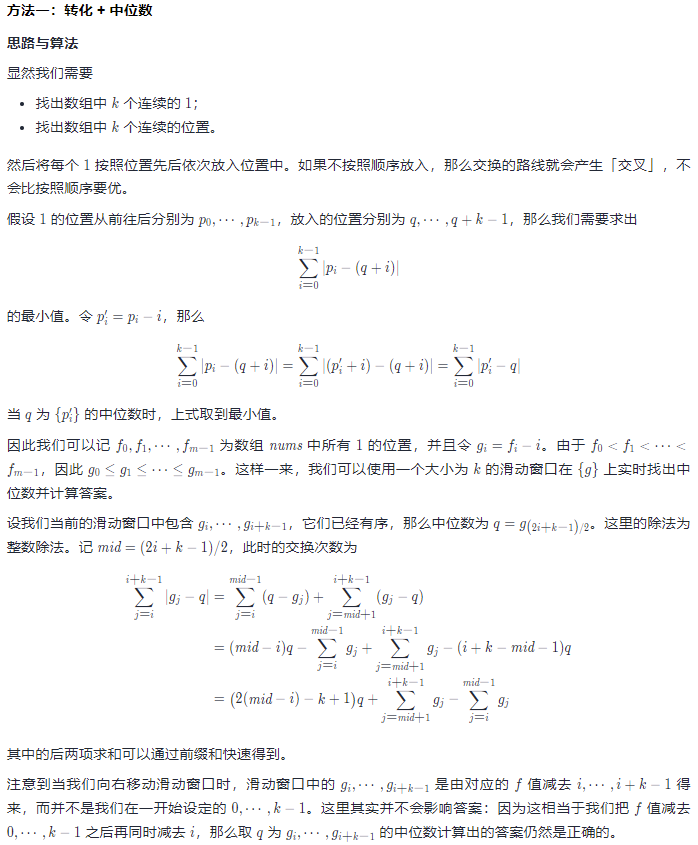
\includegraphics[width=.9\linewidth]{./pic/median.png}

\begin{minted}[fontsize=\scriptsize,linenos=false]{csharp}
public int minMoves(int[] arr, int k) {
    if (k == 1) return 0;
    int n = arr.length;
    List<Integer> g = new ArrayList<>();
    List<Integer> sum = new ArrayList<>();
    sum.add(0);
    int cnt = -1, last = 0;
    for (int i = 0; i < n; i++) {
        if (arr[i] == 0) continue;
        ++cnt;
        g.add(i-cnt);
        sum.add(last + i - cnt);
        last += i - cnt; 
    }
    int m = g.size();
    int ans = Integer.MAX_VALUE;
    for (int i = 0; i+k <= m; i++) {
        int mid = (i + i + k - 1) / 2; // 中位数下标
        int q = g.get(mid);            // 中位数
        ans = Math.min(ans, (2*(mid-i)-k+1) * q + sum.get(i+k) - sum.get(mid+1) - sum.get(mid) + sum.get(i));
    }
    return ans;
}
\end{minted}
\subsection{1838. Frequency of the Most Frequent Element - Medium}
\label{sec-5-0-8}
The frequency of an element is the number of times it occurs in an array.

You are given an integer array nums and an integer k. In one operation, you can choose an index of nums and increment the element at that index by 1.

Return the maximum possible frequency of an element after performing at most k operations.

由反证可得,在一定操作次数下最高频元素为原数组中的元素,结合贪心算法,应优先选择不大于该元素的最大数字进行递增操作。

因此,可对原数组排序后,结合双指针算法求解。设计左、右两个指针,在移动右指针的同时,维护左指针的位置,使区间内元素全部递增到右指针所在元素值的操作次数符合要求,此时区间的长度就是该元素的频率。

\begin{minted}[fontsize=\scriptsize,linenos=false]{csharp}
public int maxFrequency(int[] nums, int k) {
    int n = nums.length, ans = 1, cnt = 0;
    Arrays.sort(nums);
    for (int l = 0, r = 1; r < n; r++) {
        cnt += (nums[r] - nums[r-1]) * (r - l);// 右指针移动后所需操作次数
        while (cnt > k)                        // 操作次数超过k,移动左指针
            cnt -= nums[r] - nums[l++];
        ans = Math.max(ans, r-l+1);            // 区间长度为操作后当前元素的频数
    }
    return ans;
}
\end{minted}

\subsection{826. Most Profit Assigning Work}
\label{sec-5-0-9}
You have n jobs and m workers. You are given three arrays: difficulty, profit, and worker where:

difficulty[i] and profit[i] are the difficulty and the profit of the ith job, and
worker[j] is the ability of jth worker (i.e., the jth worker can only complete a job with difficulty at most worker[j]).
Every worker can be assigned at most one job, but one job can be completed multiple times.

For example, if three workers attempt the same job that pays \$1, then the total profit will be \$3. If a worker cannot complete any job, their profit is \$0.
Return the maximum profit we can achieve after assigning the workers to the jobs.
\begin{minted}[fontsize=\scriptsize,linenos=false]{csharp}
// 法一:暴力TreeMap---O(n^2logn)
public int maxProfitAssignment(int[] difficulty, int[] profit, int[] worker) {
    TreeMap<Integer, Integer> m = new TreeMap<>();
    for (int i = 0; i < difficulty.length; i++) 
        m.put(difficulty[i], i);
    int res = 0, idx;
    Integer low;
    for (int i = 0; i < worker.length; i++) {
        low = m.floorKey(worker[i]); // 使用treemap排序的特长
        if (low == null) continue;
        idx = m.get(low);
        for (int j = 0; j < difficulty.length; j++) 
            if (difficulty[j] <= low && profit[j] >= profit[idx])
                idx = j;
        res += profit[idx];
    }
    return res;
}
// 法二:优化的TreeMap---O(nlogn)
// 如果TreeMap里面保存的是每个difficulty[i] 对应的最大的profit,则就可以直接找floorKey对应的value就是对应的要找的value;
// 那么只需要再遍历一次TreeMap,将最大的到目前key位置最大的value放进去就行了
public int maxProfitAssignment(int[] difficulty, int[] profit, int[] worker) {
    TreeMap<Integer, Integer> m = new TreeMap<>();
    for (int i = 0; i < difficulty.length; i++) 
        m.put(difficulty[i], Math.max(m.getOrDefault(difficulty[i], 0), profit[i]));
    int max = 0;
    for (Integer key : m.keySet()) { 
        max = Math.max(max, m.get(key));
        m.put(key, max); //将最大的到目前key位置最大的value放进去
    }
    int res = 0;
    Integer low;
    for (int i = 0; i < worker.length; i++) {
        low = m.floorKey(worker[i]); // 使用treemap排序的特长
        if (low == null) continue;
        res += m.get(low);
    }
    return res;
}
// 法三:Sort + 双指针---O(nlogn)
// 思路就是先将 difficulty[]和profit组成pair,然后再将list和worker[]从小到大排序,然后遍历worker,更新tempMaxProfit,得到总的maxProfit
public int maxProfitAssignment(int[] difficulty, int[] profit, int[] worker) {
    List<int[]> list = new ArrayList<>();
    for (int i = 0; i < difficulty.length; i++) 
        list.add(new int[] {difficulty[i], profit[i]});
    Collections.sort(list, (a, b) -> {return a[0] - b[0];});
    Arrays.sort(worker);
    int res = 0, tmpMaxProfit = 0;
    // i, j同向双指针移动,更新到目前的tmpMaxProfit
    for (int i = 0, j = 0; i < worker.length; i++) {
        while (j < list.size() && list.get(j)[0] <= worker[i]) {
            tmpMaxProfit = Math.max(tmpMaxProfit, list.get(j)[1]);
            j++;
        }
        //此时tmpMaxProfit是前面所有difficulty小于worker[i]的最大的proifit
        res += tmpMaxProfit;
    }
    return res;
}
\end{minted}

\subsection{1425. Constrained Subsequence Sum - Hard}
\label{sec-5-0-10}
Given an integer array nums and an integer k, return the maximum sum of a non-empty subsequence of that array such that for every two consecutive integers in the subsequence, nums[i] and nums[j], where i < j, the condition j - i <= k is satisfied.

A subsequence of an array is obtained by deleting some number of elements (can be zero) from the array, leaving the remaining elements in their original order.

\subsection{239. Sliding Window Maximum - Hard}
\label{sec-5-0-11}
You are given an array of integers nums, there is a sliding window of size k which is moving from the very left of the array to the very right. You can only see the k numbers in the window. Each time the sliding window moves right by one position.

Return the max sliding window.

\begin{minted}[fontsize=\scriptsize,linenos=false]{csharp}
public int[] maxSlidingWindow(int[] arr, int k) {
    int n = arr.length, startWindowIdx = 0;
    ArrayDeque<Integer> q = new ArrayDeque<>(); // 维持一个递减队列
    int [] ans = new int [n - k + 1];
    for (int i = 0; i < n; i++) {
        startWindowIdx = i-k+1;
        while (!q.isEmpty() && i - q.peekFirst() >= k) q.pollFirst();     // 左出q:maintain k size window, 去头:去掉k windows之外的元素
        while (!q.isEmpty() && arr[q.peekLast()] <= arr[i]) q.pollLast(); // 右出q:去掉递减队列尾部所有不大于当前值的元素,就留一个最大值也行
        q.offerLast(i);  // 进q:进后此时q.size() == k 
        if (startWindowIdx >= 0)
            ans[startWindowIdx] = arr[q.peekFirst()]; // 使用递减队列左端最大值
    }
    return ans;
}
\end{minted}
\begin{itemize}
\item 线段树的做法
\end{itemize}
\begin{minted}[fontsize=\scriptsize,linenos=false]{csharp}
// https://blog.csdn.net/Yaokai_AssultMaster/article/details/79599809
public class MaxSeg {
    List<Integer> tree = new ArrayList<>();
    int n;
    public MaxSeg (int [] arr) {
        n = arr.length;
        tree = new ArrayList<>(2*n);
        for (int i = 0; i < n; i++) 
            tree.add(0);
        for (int i = 0; i < n; i++) 
            tree.add(arr[i]); // same effect as below
        for (int i = n-1; i >= 0; i--) // i >= 0
            tree.set(i, Math.max(tree.get(2*i), tree.get(2*i+1)));
    }
    public void update(int idx, int v) {
        idx += n;
        tree.set(idx, v);
        while (idx > 1) {
            idx /= 2;
            tree.set(idx, Math.max(tree.get(2*idx), tree.get(2*idx+1)));
        }
    }
    public int getMax(int l, int r) {
        l += n;
        r += n;
        int max = Integer.MIN_VALUE;
        while (l < r) {
            if ((l & 1) == 1) {
                max = Math.max(max, tree.get(l));
                l++;
            }
            if ((r & 1) == 1) {
                r--;            // order matters !!!
                max = Math.max(max, tree.get(r));
            }
            l >>= 1;
            r >>= 1;
        }
        return max;
    }
}
public int[] maxSlidingWindow(int[] arr, int k) {
    int n = arr.length;
    MaxSeg mat = new MaxSeg(arr);
    if (n == k) return new int [] {mat.getMax(0, n)};
    int [] res = new int [n-k+1];
    for (int i = 0; i+k <= n; i++) 
        res[i] = mat.getMax(i, i+k);
    return res;
}
\end{minted}

\subsection{双端队列:数据结构,O(N)解法类题目}
\label{sec-5-0-12}
\subsection{862. Shortest Subarray with Sum at Least K - Hard}
\label{sec-5-0-13}
Given an integer array nums and an integer k, return the length of the shortest non-empty subarray of nums with a sum of at least k. If there is no such subarray, return -1.

A subarray is a contiguous part of an array.
\begin{minted}[fontsize=\scriptsize,linenos=false]{csharp}
public int shortestSubarray(int[] nums, int k) { 
    int n = nums.length;
    int [] sum = new int[n+1];  
    for (int i = 1; i <= n; i++)  
        sum[i] = nums[i-1] + sum[i-1];
    int res = n + 1;
    ArrayDeque<Integer> q = new ArrayDeque<>(); // decreasing sum [] deque
    for (int i = 0; i <= n; i++) {
        while (!q.isEmpty() && sum[i] - sum[q.peekFirst()] >= k)  // 左出:
            res = Math.min(res, i - q.pollFirst()); // 取值了      // 取解
        while (!q.isEmpty() && sum[q.peekLast()] >= sum[i])       // 右出
            q.pollLast();  
        q.offerLast(i);                                           // 当前元素进队列
    }
    return res <= n ? res : -1;
}
\end{minted}

\subsection{1687. Delivering Boxes from Storage to Ports - Hard 滑动窗口,比较难认}
\label{sec-5-0-14}
You have the task of delivering some boxes from storage to their ports using only one ship. However, this ship has a limit on the number of boxes and the total weight that it can carry.

You are given an array boxes, where boxes[i] = [ports​​i​, weighti], and three integers portsCount, maxBoxes, and maxWeight.

ports​​i is the port where you need to deliver the ith box and weightsi is the weight of the ith box.
portsCount is the number of ports.
maxBoxes and maxWeight are the respective box and weight limits of the ship.
The boxes need to be delivered in the order they are given. The ship will follow these steps:

The ship will take some number of boxes from the boxes queue, not violating the maxBoxes and maxWeight constraints.
For each loaded box in order, the ship will make a trip to the port the box needs to be delivered to and deliver it. If the ship is already at the correct port, no trip is needed, and the box can immediately be delivered.
The ship then makes a return trip to storage to take more boxes from the queue.
The ship must end at storage after all the boxes have been delivered.

Return the minimum number of trips the ship needs to make to deliver all boxes to their respective ports.
\begin{enumerate}
\item 解题思路与分析: 滑动窗口
\label{sec-5-0-14-1}
\begin{itemize}
\item 这里会需要一种决策:需要总运送次数最少,就涉及到同一船是否只装送往同一个港口的优化与选择问题,用滑动窗口,也有贪心的解法
\item 时间复杂度: O(N)
\end{itemize}
\begin{minted}[fontsize=\scriptsize,linenos=false]{csharp}
public int boxDelivering(int[][] box, int __, int max, int limit) {
    int n = box.length;
    int[] dp = new int[n+1]; // Minimum trips for first n boxes.
    int wit = 0, cost = 2;   // cumulative weight, cumulative cost
    int l = 0;                   // left ptr
    for (int r = 0; r < n; r++) {// right ptr
        wit += box[r][1];
        if (r > 0 && box[r][0] != box[r-1][0]) cost++; // 现箱子与上一个箱子运往的目的地不同
        /* drop box iff:
           - There are too many box (r-l >= max)
           - The box are too heavy (weight > limit)
           - It is redundant to carry them (dp[l] == dp[l+1]).
        */                                 // 送往同一个港口的箱子向右滑动,直到改变消耗的临界点
        while (r - l >= max || wit > limit || (l < r && dp[l] == dp[l+1])) { // 滑动窗口:左窗口右移
            wit -= box[l][1];
            if (box[l+1][0] != box[l][0]) cost--;
            l++;
        }
        dp[r+1] = cost + dp[l]; // 运完下标为 r 的箱子后的最小次数,对应 dp[r+1]
    }
    return dp[n];
}
\end{minted}
\begin{itemize}
\item 一种dp的写法,写得天外来仙,可惜不是很好懂
\end{itemize}
\begin{minted}[fontsize=\scriptsize,linenos=false]{csharp}
public int boxDelivering(int [][] box, int portsCount, int maxBox, int maxWeight) {
    int n = box.length, j = 0, lastj = 0, cnt = 0; // cnt: cost
    int [] dp = new int [n+1];
    Arrays.fill(dp, Integer.MAX_VALUE / 2);
    dp[0] = 0;
    for (int i = 0; i < n; i++) {
        while (j < n && maxBox > 0 && maxWeight >= box[j][1]) {
            maxBox -= 1;
            maxWeight -= box[j][1];
            if (j == 0 || box[j][0] != box[j-1][0]) {
                lastj = j; // 新目的地港口的第一个下标
                cnt++; // 增加消耗
            }
            ++j; // keep expanding the right pointer when we can 右窗口尽可能地向右延伸:只要有空间,延伸至最远
        }
        dp[j] = Math.min(dp[j], dp[i] + cnt + 1);
        dp[lastj] = Math.min(dp[lastj], dp[i] + cnt);
        // 随着i的增加,左窗口右移:移走第i个箱子所腾出的空间(箱子个安数、重量,以及潜在可能减少的一次消耗)都需要更新
        maxBox += 1; // now as we move the left pointer i forward (don't put the ith box in this trip),
        maxWeight += box[i][1];  // we increase the number of available boxes and available weights
        if (i == n-1 || box[i][0] != box[i+1][0]) cnt--;
    }
    return dp[n];
}
\end{minted}
\end{enumerate}

\subsection{992. Subarrays with K Different Integers - Hard}
\label{sec-5-0-15}
Given an integer array nums and an integer k, return the number of good subarrays of nums.

A good array is an array where the number of different integers in that array is exactly k.

For example, [1,2,3,1,2] has 3 different integers: 1, 2, and 3.
A subarray is a contiguous part of an array.
\begin{enumerate}
\item 解题思路与分析
\label{sec-5-0-15-1}
\begin{itemize}
\item 思路依然是滑动窗口,但是这一题是没法直接套用76题的模板的,有一些变动(引用)。回忆前面做的滑动窗口的题目,有求过子数组里面最多K个不同元素的题(340),所以这个解法的思路是求子数组里面最多K个不同元素的子数组的数量 - 子数组里面最多K - 1个不同元素的子数组的数量。
\end{itemize}
\begin{minted}[fontsize=\scriptsize,linenos=false]{csharp}
private int atMostK(int [] arr, int k) {
    int ans = 0, l = 0;                    // Left boundary of window
    Map<Integer, Integer> cnt = new HashMap<>(); // Map to keep track of number of distinct elements in the current window
    for (int i = 0; i < arr.length; i++) { // i : right
        cnt.put(arr[i], cnt.getOrDefault(arr[i], 0) + 1);
        while (cnt.size() > k) {
            if (cnt.get(arr[l]) > 1) cnt.put(arr[l], cnt.get(arr[l])-1);
            else cnt.remove(arr[l]);
            l++;
        }
        ans += i - l + 1; // Adding the count of subarrays with at most K distinct elements in the current window
    }
    return ans;
}
public int subarraysWithKDistinct(int[]arr, int k) {
    return atMostK(arr, k) - atMostK(arr, k-1);
}
\end{minted}
\end{enumerate}

\subsection{1438. Longest Continuous Subarray With Absolute Diff Less Than or Equal to Limit - Medium 双端队列}
\label{sec-5-0-16}
Given an array of integers nums and an integer limit, return the size of the longest non-empty subarray such that the absolute difference between any two elements of this subarray is less than or equal to limit.
\begin{enumerate}
\item 解题思路与分析
\label{sec-5-0-16-1}
\begin{itemize}
\item 如果使用普通列表再排序的话会增加一个logn的时间复杂度,会超时!
\item 选对了数据类型后,直接套滑窗模板即可,简单的一。。。
\item Intuition:
\end{itemize}
\begin{minted}[fontsize=\scriptsize,linenos=false]{csharp}
 . we can use siliding window but we need to keep track of minimum and maximum in every window 
 . treemap can be used for this purpose to keep track of min and max both
\end{minted}
\begin{itemize}
\item 这是一种临场应对的偷懒解法,选对数据结构,牺牲一点儿效率,但是可以最大限度地保证结果的正确性
\end{itemize}
\begin{minted}[fontsize=\scriptsize,linenos=false]{csharp}
// Time complexity: O(N*LogN), insertion in treeMap is logN and for N elements it is O(N*LogN)
// Auxiliary Space: O(N), every key enters the map once and in worst case every key can be present with frequency one
public int longestSubarray(int[] arr, int limit) { // TreeMap to keep Min & Max at O(NlogN)
    TreeMap<Integer, Integer> cnt = new TreeMap<>();
    int l = 0, r = 0;
    while (r < arr.length) {
        cnt.put(arr[r], cnt.getOrDefault(arr[r], 0) + 1);
        if (cnt.lastEntry().getKey() - cnt.firstEntry().getKey() > limit) {
            if (cnt.get(arr[l]) > 1)
                cnt.put(arr[l], cnt.get(arr[l])-1);
            else cnt.remove(arr[l]);
            l++;
        }
        r++;
    }
    return r - l; // 这样维护的就是全局最优解了?!!!
}
\end{minted}
\begin{itemize}
\item 但是在平时练习时,还是要不断地寻求最优解,使用双端队列,得O(N)线性复杂度
\item Intuition:
\end{itemize}
\begin{minted}[fontsize=\scriptsize,linenos=false]{csharp}
// . we can use siliding window but we need to keep track of minimum and maximum in every window 
// . 2 Deques can be used for this purpose to keep track of min and max.
// Time complexity: O(N), N is number of elements in nums
// Auxiliary Space: O(N)
public int longestSubarray(int[] nums, int limit) { // 双端队列:从右边加入
    ArrayDeque<Integer> min = new ArrayDeque<>();   // 单调递增队列: 左小右大
    ArrayDeque<Integer> max = new ArrayDeque<>();   // 单调递减队列: 左大右小
    int l = 0, r = 0, ans = 0;
    while (r < nums.length) {
        int rval = nums[r];
//to ensure that minQ have minimum element as head             
        while (!min.isEmpty() && min.peekLast() > rval) min.pollLast(); // 维护:右边,比当前待入列值大的,全扔出去
//to ensure that maxQ have maximum element as head                
        while (!max.isEmpty() && max.peekLast() < rval) max.pollLast(); // 维护:右边,比当前待入列值小的,全扔出去                
        min.offerLast(rval); // 入队列,从右边加入
        max.offerLast(rval); // 
//In case max-min is greater than the limit slide the left side or window         
        if (max.peekFirst() - min.peekFirst() > limit) {     // 维护合法窗口范围: 会两个队列都把 l 下标的值抓不出去吗?
            if (min.peekFirst() == nums[l]) min.pollFirst(); // 
            if (max.peekFirst() == nums[l]) max.pollFirst(); // 
            l++;
        }
        r++;
    }
    return r - l;
}
\end{minted}
\begin{itemize}
\item 另一种把它"刷"过去的应付的写法(MinSeg, MaxSeg列在这里,方便自己以后参考时查找)
\end{itemize}
\begin{minted}[fontsize=\scriptsize,linenos=false]{csharp}
public class MaxSeg {
    List<Integer> tree = new ArrayList<>();
    int n;
    public MaxSeg (int [] arr) {
        n = arr.length;
        tree = new ArrayList<>(2 * n);
        for (int i = 0; i < n; i++)
            tree.add(0);
        for (int i = 0; i < n; i++)
            tree.add(arr[i]); // same effect as below
        for (int i = n-1; i >= 0; i--) // i >= 0
            tree.set(i, Math.max(tree.get(2 * i), tree.get(2 * i+1)));
    }
    public void update(int idx, int v) {
        idx += n;
        tree.set(idx, v);
        while (idx > 1) {
            idx /= 2;
            tree.set(idx, Math.max(tree.get(2 * idx), tree.get(2 * idx+1)));
        }
    }
    public int getMax(int l, int r) {
        l += n;
        r += n;
        int max = Integer.MIN_VALUE;
        while (l < r) {
            if ((l & 1) == 1) {
                max = Math.max(max, tree.get(l));
                l++;
            }
            if ((r & 1) == 1) {
                r--; // order matters !!!
                max = Math.max(max, tree.get(r));
            }
            l >>= 1;
            r >>= 1;
        }
        return max;
    }
}        
public class MinSeg {
    List<Integer> tree = new ArrayList<>();
    int n;
    public MinSeg (int [] arr) {
        n = arr.length;
        tree = new ArrayList<>(2*n);
        for (int i = 0; i < n; i++) 
            tree.add(0);
        for (int i = 0; i < n; i++) 
            tree.add(arr[i]); 
        for (int i = n-1; i >= 0; i--)  // i >= 0
            tree.set(i,  Math.min(tree.get(2*i),  tree.get(2*i+1)));
    }
    public void update(int idx,  int v) {
        idx += n;
        tree.set(idx,  v);
        while (idx > 1) {
            idx /= 2;
            tree.set(idx,  Math.min(tree.get(2*idx),  tree.get(2*idx+1)));
        }
    }
    public int getMin(int l,  int r) { // [l, r) include left, not included right
        l += n;
        r += n;
        int min = Integer.MAX_VALUE;
        while (l < r) {
            if ((l & 1) == 1) {
                min = Math.min(min,  tree.get(l));
                l++;
            }
            if ((r & 1) == 1) {
                r--; // order matters !!!
                min = Math.min(min,  tree.get(r));
            }
            l >>= 1;
            r >>= 1;
        }
        return min;
    }
}
public int longestSubarray(int[] arr, int limit) { // 单调递增队列,左小右大,右进左出 
    MaxSeg max = new MaxSeg(arr);
    MinSeg min = new MinSeg(arr);
    int res = 0, tmp = 0, j = 0;
    int n = arr.length;
    for (int i = 1; i <= n; i++) {
        if (max.getMax(j, i) - min.getMin(j, i) <= limit) {
            tmp = i-j;
            res = Math.max(res, tmp);
        } else 
            while (max.getMax(j, i) - min.getMin(j, i) > limit && j < i) ++j;
    }
    return res;
}
\end{minted}
\end{enumerate}
\subsection{1493. Longest Subarray of 1's After Deleting One Element - Medium}
\label{sec-5-0-17}
Given a binary array nums, you should delete one element from it.

Return the size of the longest non-empty subarray containing only 1's in the resulting array. Return 0 if there is no such subarray.
\begin{enumerate}
\item 解题思路与分析: 滑动窗口 O(N)
\label{sec-5-0-17-1}

是滑动窗口的题目,以后比赛的时候就这么写,自己数下标,数得累死还bug满天飞,借助一个双端队列,至少自动过滤掉不少bug

\begin{minted}[fontsize=\scriptsize,linenos=false]{csharp}
public int longestSubarray(int[] a) {
    int n = a.length, cnt = 0, i = 0, max = 0;
    ArrayDeque<Integer> q = new ArrayDeque<>();
    boolean hasO = false; // {0, 0, 1, 1} 这个特例不能忘记了
    while (i < n && a[i] == 0) {
        hasO = true;
        i++;
    }
    if (i == n) return 0;
    for (; i < n; i++) {
        q.offerLast(a[i]);
        if (a[i] == 0) {
            cnt++;
            if (cnt == 2) {
                max = Math.max(max, q.size()-cnt);
                while (!q.isEmpty() && q.peek() != 0) q.pollFirst();
                q.pollFirst();
                cnt--;
            }
        }
    }
    if (a[n-1] == 1) max = Math.max(max, q.size()-(cnt > 0 ? cnt : (hasO ? 0 : 1)));
    else max = Math.max(max, q.size()-cnt);
    return max;
}
\end{minted}
\begin{itemize}
\item 贴个别人真正的滑动窗口的代码
\end{itemize}
\begin{minted}[fontsize=\scriptsize,linenos=false]{cpp}
int longestSubarray(vector<int>& nums) {
    const int n = nums.size();
    int ans = 0;
    int sum = 0; // sum of nums[l~r].
    for (int l = 0, r = 0; r < n; ++r) {
        sum += nums[r];
        while (l < r && sum < r - l) // Maintain sum >= r - l, at most 1 zero.
            sum -= nums[l++];
        ans = max(ans, r - l);
    }
    return ans;
}
\end{minted}
\item 解题思路与分析: 双变量
\label{sec-5-0-17-2}

早上的时候不是刚写过一个这样的题吗 ? 与926 的第二种解法有什么区别? 

\begin{minted}[fontsize=\scriptsize,linenos=false]{csharp}
// count1:当前包含一个非1的连续长度。
// count2:当前全是1的连续长度。
// 循环数组每一个数字,如果当前数字是1,count1和count2同时加一,同时使用count1更新全局最大值。
// 重点来了,如果当前数字是非1,则设count1等于count2,count2设为0。最后处理一下全是1的特例即可。
public int longestSubarray(int[] a) { // bug出多了,自己也能悟出来:数据结构帮大忙:
    int n = a.length, ans = 0, cnt = 0, one = 0, zoo = 0;
    for (Integer v : a) {
        if (v == 0) {
            zoo++;
            cnt = one;
            one = 0;
        } else {
            cnt++;
            one++;
            ans = Math.max(ans, cnt);
        }
    }
    return ans == n ? n-1 : ans;
}
\end{minted}
\item 解题思路与分析: DP
\label{sec-5-0-17-3}
Preprocess:

l[i] := longest 1s from left side ends with nums[i], l[i] = nums[i] + nums[i] * l[i – 1]

r[i] := longest 1s from right side ends with nums[i], r[i] = nums[i] + nums[i] * r[i + 1]

Use each node as a bridge (ignored), the total number of consecutive 1s = l[i – 1] + r[i + 1].

ans = max\{l[i-1] + r[i +1]\}

Time complexity: O(n)

Space complexity: O(n)
\begin{minted}[fontsize=\scriptsize,linenos=false]{cpp}
int longestSubarray(vector<int>& nums) {
    const int n = nums.size();
    vector<int> l(n);
    vector<int> r(n);
    for (int i = 0; i < n; ++i)
        l[i] = (i > 0 ? l[i - 1] * nums[i] : 0) + nums[i];
    for (int i = n - 1; i >= 0; --i)
        r[i] = (i < n - 1 ? r[i + 1] * nums[i] : 0) + nums[i];
    int ans = 0;
    for (int i = 0; i < n; ++i)
        ans = max(ans, (i > 0 ? l[i - 1] : 0) + 
                       (i < n - 1 ? r[i + 1] : 0));
    return ans;
}
\end{minted}
\item 解题思路与分析
\label{sec-5-0-17-4}
\begin{minted}[fontsize=\scriptsize,linenos=false]{csharp}
dp[i][0] := longest subarray ends with nums[i] has no ones.
dp[i][0] := longest subarray ends with nums[i] has 1 one.
if nums[i] == 1:
dp[i][0] = dp[i – 1][0] + 1
dp[i][1] = dp[i – 1][1] + 1
if nums[i] == 0:
dp[i][0] = 0
dp[i][1] = dp[i – 1][0] + 1
\end{minted}

Time complexity: O(n)

Space complexity: O(n) -> O(1)

\begin{minted}[fontsize=\scriptsize,linenos=false]{cpp}
int longestSubarray(vector<int>& nums) {
    const int n = nums.size();
    // dp[i][0] := longest subarray ends with nums[i-1] has no zeros.
    // dp[i][0] := longest subarray ends with nums[i-1] has 1 zero.
    vector<vector<int>> dp(n + 1, vector<int>(2));
    int ans = 0;
    for (int i = 1; i <= n; ++i) {
        if (nums[i - 1] == 1) {
            dp[i][0] = dp[i - 1][0] + 1;
            dp[i][1] = dp[i - 1][1] + 1;
        } else {
            dp[i][0] = 0;
            dp[i][1] = dp[i - 1][0] + 1;
        }
        ans = max({ans, dp[i][0] - 1, dp[i][1] - 1});
    }
    return ans;
}
\end{minted}
\end{enumerate}

\subsection{857. Minimum Cost to Hire K Workers - Hard}
\label{sec-5-0-18}
There are n workers. You are given two integer arrays quality and wage where quality[i] is the quality of the ith worker and wage[i] is the minimum wage expectation for the ith worker.

We want to hire exactly k workers to form a paid group. To hire a group of k workers, we must pay them according to the following rules:

Every worker in the paid group should be paid in the ratio of their quality compared to other workers in the paid group.
Every worker in the paid group must be paid at least their minimum wage expectation.
Given the integer k, return the least amount of money needed to form a paid group satisfying the above conditions. Answers within 10-5 of the actual answer will be accepted.
\begin{enumerate}
\item 解题思路与分析
\label{sec-5-0-18-1}
\begin{itemize}
\item 做题的时候没有想明白,为什么不是性价比最低的k个工人,什么情况下性价比最低的k个工人不是题目要求的答案?
\item 时间复杂度O ( n log ⁡ n ),空间O ( n ) 。
\end{itemize}
\begin{minted}[fontsize=\scriptsize,linenos=false]{csharp}
public double mincostToHireWorkers(int[] quality, int[] wage, int k) {
    int n = quality.length;
    List<int []> l = new ArrayList<>();
    for (int i = 0; i < n; i++) {
        int [] cur = new int [] {wage[i], quality[i]};
        l.add(cur);
    }
    Collections.sort(l, (a, b) -> Double.compare((double)a[0] / a[1], (double)b[0] / b[1]));
    Queue<Integer> q = new PriorityQueue<>((x, y) -> -Integer.compare(x, y)); // 堆里存所以t值小于等于当前枚举的t值的工人中,q值最小的k个人的q值
    double res = 1e18, sum = 0;
    for (int i = 0; i < n; i++) {
        int [] cur = l.get(i);
        sum += cur[1];
        q.offer(cur[1]);
        if (q.size() > k)
            sum -= q.poll();
        if (q.size() == k)
            res = Math.min(res, sum * (double)cur[0] / (double)cur[1]);
    }
    return res;
}
\end{minted}
\end{enumerate}

\subsection{480 Sliding Window Median}
\label{sec-5-0-19}
The median is the middle value in an ordered integer list. If the size of the list is even, there is no middle value. So the median is the mean of the two middle values.
For examples, if arr = [2,3,4], the median is 3.
For examples, if arr = [1,2,3,4], the median is (2 + 3) / 2 = 2.5.
You are given an integer array nums and an integer k. There is a sliding window of size k which is moving from the very left of the array to the very right. You can only see the k numbers in the window. Each time the sliding window moves right by one position.
Return the median array for each window in the original array. Answers within 10-5 of the actual value will be accepted.
\begin{minted}[fontsize=\scriptsize,linenos=false]{csharp}
public double[] medianSlidingWindow(int[] nums, int k) {
    TreeMap<Integer, Integer> ma = new TreeMap<>();
    TreeMap<Integer, Integer> mb = new TreeMap<>();
    for (int i = 0; i < k; i++) {
        if (i % 2 == 0) {
            mb.put(nums[i], mb.getOrDefault(nums[i], 0) + 1);
            int n = mb.firstKey();
            if (mb.get(n) == 1) mb.remove(n);
            else mb.put(n, mb.get(n) - 1);
            ma.put(n, ma.getOrDefault(n, 0) + 1);
        } else {
            ma.put(nums[i], ma.getOrDefault(nums[i], 0) + 1);
            int n = ma.lastKey();
            if (ma.get(n) == 1) ma.remove(n);
            else ma.put(n, ma.get(n) - 1);
            mb.put(n, mb.getOrDefault(n, 0) + 1);
        }
    }
    double [] res = new double[nums.length-k+1];
    if (k % 2 == 1) res[0] = ma.lastKey();
    else res[0] =  (double)(((long)(ma.lastKey()) + (long)(mb.firstKey())) / 2.0);
    for (int i = 0; i + k < nums.length; i++) {
        ma.put(nums[i+k], ma.getOrDefault(nums[i+k], 0) + 1);
        int n = ma.lastKey();
        if (ma.get(n) == 1) ma.remove(n);
        else ma.put(n, ma.get(n) - 1);
        mb.put(n, mb.getOrDefault(n, 0) + 1);
        if (ma.containsKey(nums[i])) {
            if (ma.get(nums[i]) == 1) ma.remove(nums[i]);
            else ma.put(nums[i], ma.get(nums[i]) - 1);
            int v = mb.firstKey();
            if (mb.get(v) == 1) mb.remove(v);
            else mb.put(v, mb.get(v) - 1);
            ma.put(v, ma.getOrDefault(v, 0) + 1);
        } else {
            if (mb.get(nums[i]) == 1) mb.remove(nums[i]);
            else mb.put(nums[i], mb.get(nums[i]) - 1);
        }
        if (k % 2 == 1) res[i+1] = ma.lastKey();
        else res[i+1] = (double)(((long)(ma.lastKey()) + (long)(mb.firstKey())) / 2.0);
    }
    return res;
}
\end{minted}

\chapter{TreeMap}
\label{sec-6}
\section{2382. Maximum Segment Sum After Removals - Hard}
\label{sec-6-1}
You are given two 0-indexed integer arrays nums and removeQueries, both of length n. For the ith query, the element in nums at the index removeQueries[i] is removed, splitting nums into different segments.

A segment is a contiguous sequence of positive integers in nums. A segment sum is the sum of every element in a segment.

Return an integer array answer, of length n, where answer[i] is the maximum segment sum after applying the ith removal.

Note: The same index will not be removed more than once.
\subsection{思路分析}
\label{sec-6-1-1}
\begin{itemize}
\item Using simple logic of storing the ranges and splitting them as solving the query.
\item Intially, we will be having whole array as are range (0, n-1). Now as we solve queries, say remove index x or set index x value as 0, we will split our range into (0, x -1) and (x + 1, n). Also, we will remove our previous range as it is of no use.
\item There can be cases in that, suppose we need to remove x and there is range (x, x), then we will simple remove it and not adding anything back (refer code below)
\item Now, to get the maximum sum of all the possible ranges, we will use another treemap, which will store sum to its frequency (frequency because multiple ranges can have same sum). And we can fetch maximum sum at any point in O(1) by simple getting last element of treemap.
\end{itemize}
\begin{minted}[fontsize=\scriptsize,linenos=false]{csharp}
public long[] maximumSegmentSum(int[] a, int[] q) {
    int n = a.length;
    long [] sum = new long [n+1], ans = new long [n];
    for (int i = 0; i < n; i++) // calc preSum
        sum[i+1] = sum[i] + a[i];
    TreeMap<int [], Long> m = new TreeMap<>((x, y)->x[0] - y[0]); // 这里定义了一个相对独特的比较方式  ranges
    // TreeMap to store all the possible sums of range we encounter while solving queries, we are storing frequencies because 
    // multiple range can have same sum.            
    TreeMap<Long, Integer> sums = new TreeMap<>(); 
    m.put(new int [] {0, n-1}, sum[n]);
    sums.put(sum[n], 1);
    for (int i = 0; i < n; i++) {
        int v = q[i];
        // finding range which will split when node index is removed or set 0.                
        int [] rangeToBeRemoved = m.floorKey(new int [] {v}); // 所以数组的长短都没有关系
        Long sumv =m.get(rangeToBeRemoved);
        // removing/ reducing sum from sums Map because we are splitting that range, so it is no longer valid
        int freq = sums.get(sumv);
        if (freq == 1) sums.remove(sumv);
        else sums.put(sumv, freq-1);
        m.remove(rangeToBeRemoved); // removing that range
        int l = rangeToBeRemoved[0], r = rangeToBeRemoved[1];
        long curSum = 0;
        // Splitting range and store back new ranges form along with its sum.
        if (l == v && r != v) { // 更新当前分割点右边的片段
            curSum = sum[r+1] - sum[v+1];
            m.put(new int [] {v+1, r}, curSum);
            sums.put(curSum, sums.getOrDefault(curSum, 0) + 1);
        } else if (l != v && r == v) { // 更新当前分割点左边的片段
            curSum = sum[v] - sum[l];
            m.put(new int [] {l, v-1}, curSum);
            sums.put(curSum, sums.getOrDefault(curSum, 0) + 1);
        } else if (l < v && r > v) {
            // 左边
            curSum = sum[v] - sum[l];
            m.put(new int [] {l, v-1}, curSum);
            sums.put(curSum, sums.getOrDefault(curSum, 0) + 1);
            // 右边
            curSum = sum[r+1] - sum[v+1];
            m.put(new int [] {v+1, r}, curSum);
            sums.put(curSum, sums.getOrDefault(curSum, 0) + 1);
        }
        if (sums.size() !=  0)
            ans[i] = sums.lastKey();
    }
    return ans;
}
\end{minted}
\begin{itemize}
\item 另外一个想起来相对简单的思路
\begin{minted}[fontsize=\scriptsize,linenos=false]{csharp}
public long[] maximumSegmentSum(int[] a, int[] qr) {
    int n = a.length;
    Queue<long []> q = new PriorityQueue<>((x, y) -> x[2] <= y[2] ? 1 : -1); // 转化成int值
    TreeSet<Integer> s = new TreeSet<>();
    long [] sum = new long [n], ans = new long [n];
    s.add(-1); // qr[i] in range [0, n)
    s.add(n);
    for (int i = 0; i < n; i++) {
        sum[i] = a[i];
        if (i > 0) sum[i] += sum[i-1];
    }
    q.offer(new long [] {0, n-1, sum[n-1]}); // [ bgn, end ], sum of segment
    for (int i = 0; i < n; i++) {
        int v = qr[i];
        s.add(v);
// 先添加可能会产生的分割点左右的两个新片段;再从QUEUE里移除含有当前分割点的一个片段,或是直接读最大有效值                
        // l, r: left, right, 比当前分割点小的最大值,和比当前分割点大的最小值
        int l = s.lower(v), r = s.higher(v); 
        if (l + 1 < v) // 比当前分割点小的可以产生段新的片段
            q.offer(new long [] {(long)l + 1, (long)v - 1, sum[v-1] - (long)(l == -1 ? 0 : sum[l])}); // - sum[l]
        if (v + 1 < r) // 比当前分割点大的也可以产生一段新的片段
            q.offer(new long [] {(long)v+1, (long)r-1, sum[r-1] - sum[v]}); // - sum[v]
        while (!q.isEmpty()) {
            long [] cur = q.peek();
            int bgn = (int)cur[0], end = (int)cur[1];
            // 根据当前片段的两个端点值来确认:当前片段是有效片段,取第一个有效片段读值
            if (s.higher(bgn-1) > end) {
                ans[i] = q.peek()[2];
                break;
            } else q.poll(); // 如果是无效片段,就把它扔掉
        }
    }
    return ans;
}
\end{minted}
\end{itemize}
\chapter{HashMap}
\label{sec-7}
\subsection{数有多少个数组数不清楚}
\label{sec-7-0-1}
\subsection{1392. Longest Happy Prefix - Hard KMP算法 - 这个题需要重写}
\label{sec-7-0-2}
A string is called a happy prefix if is a non-empty prefix which is also a suffix (excluding itself).

Given a string s, return the longest happy prefix of s. Return an empty string "" if no such prefix exists.
\begin{minted}[fontsize=\scriptsize,linenos=false]{csharp}
// 频繁的字符串操作(substring和equals操作)会大幅消耗执行时间,也会导致TLE时间超时。
// 因此我们可以使用字符串的hash值方式来比较前后缀是否相同。这里我们需要普及一个知识点,任意一个字符串的Hash值的计算公式为:
// int hash=s[0]∗31^(n−1)+s[1]∗31^(n−2) +...+s[n−2]∗31^1+s[n−1]∗31^0
//     对于前缀hash,每次长度加一后hash的变化应该是:
//     hash = hash*31 + 新添头字符ch
//     对于后缀hash,每次长度加一后hash的变化应该是:
//     hash = hash + 新添尾字符*31^t   (t为后缀长度减1)
//     这样我们每次只需要比较前缀hash与后缀hash是否相同即可。
public String longestPrefix(String s) {
    int n = s.length(), hashPre = 0, hashSuf = 0;
    int left = 0, right = n-1, pow = 1, maxLen = 0;
    String res = "";
    while (left < n-1) {
        hashPre = hashPre * 31 + s.charAt(left);
        hashSuf = hashSuf + s.charAt(right)*pow;
        if (hashPre == hashSuf) maxLen = left + 1;
        left ++;
        right --;
        pow *= 31;
    }
    return maxLen == 0 ? "" : s.substring(0, maxLen);
}
\end{minted}
\begin{enumerate}
\item 解题思路与分析
\label{sec-7-0-2-1}
\begin{itemize}
\item 利用字典wmap保存单词 -> 下标的键值对
\item 遍历单词列表words,记当前单词为word,下标为idx:
\end{itemize}
\begin{minted}[fontsize=\scriptsize,linenos=false]{csharp}
1). 若当前单词word本身为回文,且words中存在空串,则将空串下标bidx与idx加入答案
2). 若当前单词的逆序串在words中,则将逆序串下标ridx与idx加入答案
3). 将当前单词word拆分为左右两半left,right。
     3.1) 若left为回文,并且right的逆序串在words中,则将right的逆序串下标rridx与idx加入答案
     3.2) 若right为回文,并且left的逆序串在words中,则将left的逆序串下标idx与rlidx加入答案
\end{minted}

情况分析清楚以后,针对每个情况逐个判断, 然后提前建好hashmap以后判断就好。

细节部分是不要忘记空字符串的情况, 然后针对整个字符串反过来的情况,不要有重复。
\begin{minted}[fontsize=\scriptsize,linenos=false]{csharp}
private boolean isPalindrome(String s, int i, int j) {
    while (i < j) 
        if (s.charAt(i++) != s.charAt(j--)) return false;
    return true;
}
public List<List<Integer>> palindromePairs(String[] words) {
    Map<String, Integer> map = new HashMap<>();
    List<List<Integer>> ans = new ArrayList<>();
    for (int i = 0; i < words.length; i++) 
        map.put(words[i], i);
    for (int i = 0; i < words.length; i++) {
        if (words[i].equals("")) {
            for (int j = 0; j < words.length; j++) {
                String w = words[j];
                if (isPalindrome(w, 0, w.length()-1) && j != i) {
                    ans.add(List.of(i, j));
                    ans.add(List.of(j, i));
                }
            }
            continue;
        }
        StringBuilder sb = new StringBuilder(words[i]);
        sb.reverse();
        String bw = sb.toString();
        if (map.containsKey(bw)) {
            int res = map.get(bw);
            if (res != i) ans.add(List.of(i, res));
        }
        for (int j = 1; j < bw.length(); j++) {
            if (isPalindrome(bw, 0, j-1)) {
                String s = bw.substring(j);
                if (map.containsKey(s))
                    ans.add(List.of(i, map.get(s)));
            }
            if (isPalindrome(bw, j, bw.length()-1)) {
                String s = bw.substring(0, j);
                if (map.containsKey(s))
                    ans.add(List.of(map.get(s), i));
            }
        }
    }
    return ans;
}
\end{minted}

\item KMP 算法
\label{sec-7-0-2-2}
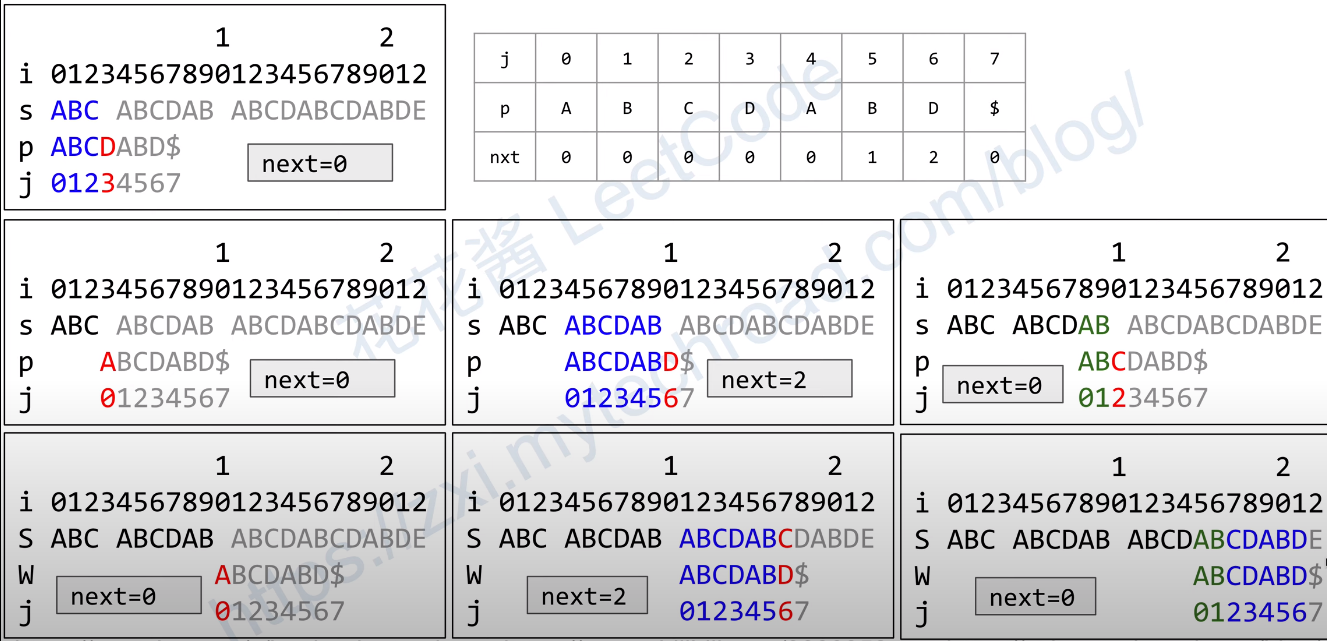
\includegraphics[width=.9\linewidth]{./pic/kmp.png}

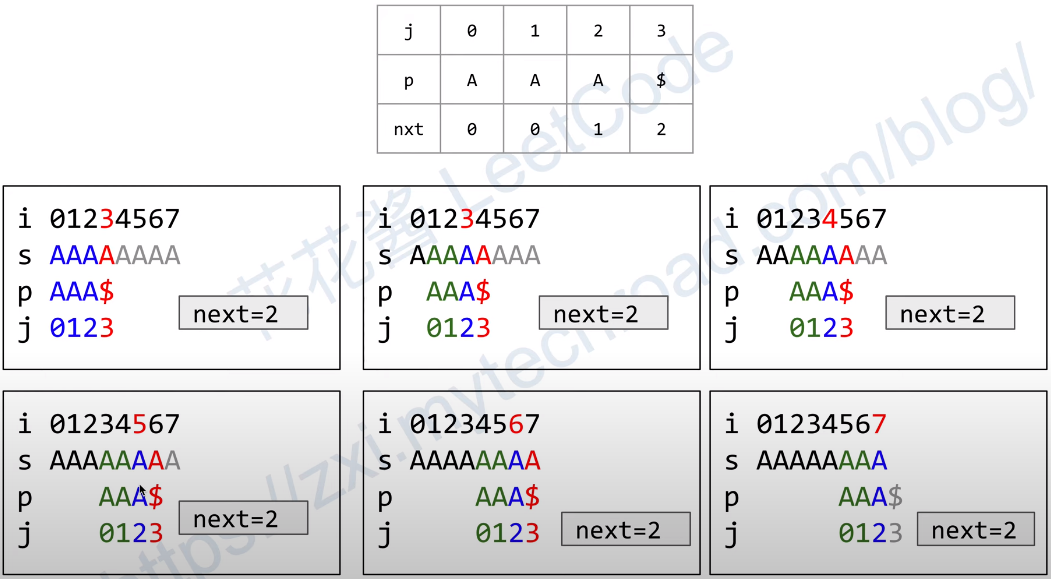
\includegraphics[width=.9\linewidth]{./pic/kmp2.png}

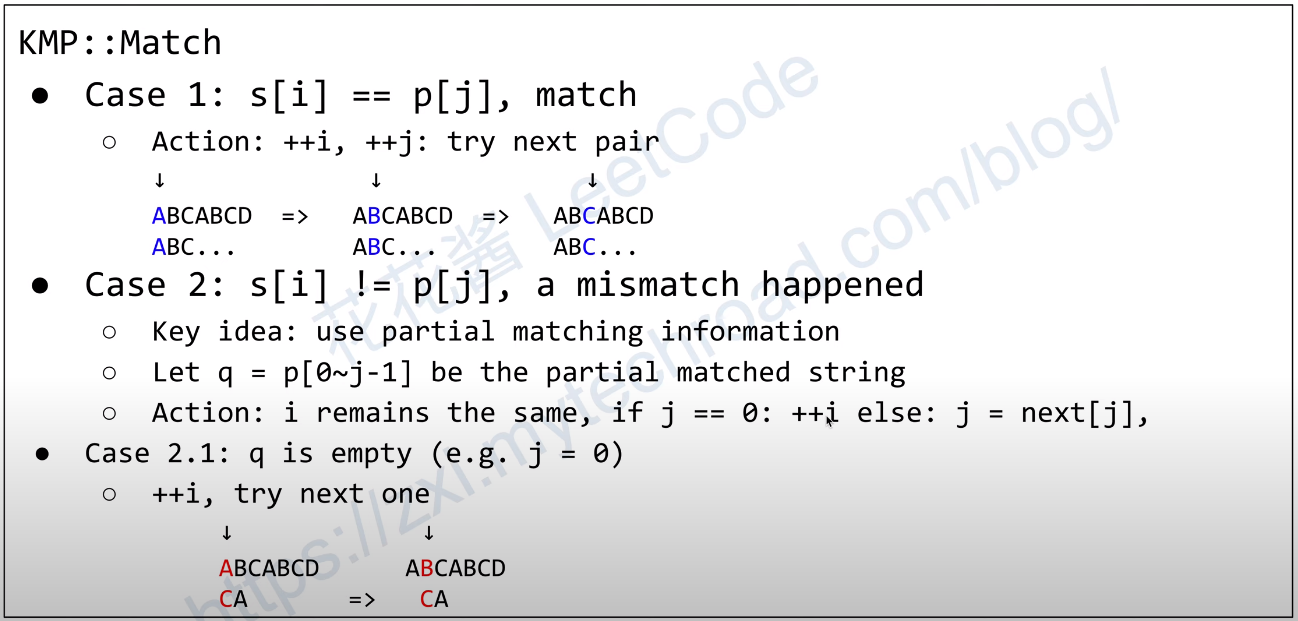
\includegraphics[width=.9\linewidth]{./pic/kmp3.png}

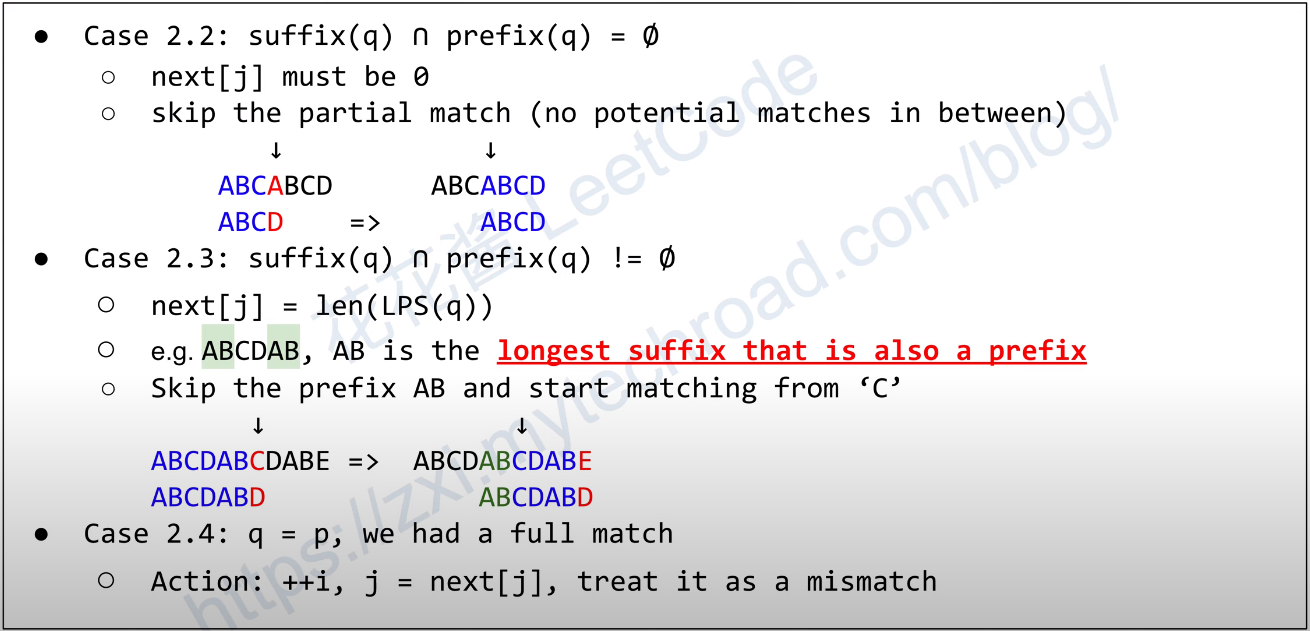
\includegraphics[width=.9\linewidth]{./pic/kmp4.png}

\begin{minted}[fontsize=\scriptsize,linenos=false]{csharp}
// straight forward KMP algorithm - 8ms - beats 94% time - O(N) time and O(N) space
public String longestPrefix(String s) {
    int i, x, N = s.length();
    int [] LPS = new int[N];
    LPS[0] = 0;
    for (i = 1; i < N; i++){
        x = LPS[i - 1];
        while (s.charAt(i) != s.charAt(x)){
            if (x == 0){
                x = -1;
                break;
            }
            x = LPS[x - 1];
        }
        LPS[i] = x + 1;
    }
    return s.substring(0, LPS[N - 1]);
}
\end{minted}
\begin{minted}[fontsize=\scriptsize,linenos=false]{cpp}
string longestPrefix(string s) {
    vector<int> lps(s.size(), 0);
    size_t i = 0, j = 1;
    while (j < s.size()) {
        if (s[i] == s[j]) lps[j++] = (i++) + 1;  // situ.1
        else if (i != 0) i = lps[i - 1];         // situ.2
        else lps[j++] = 0;                       // situ.3
    }
    return s.substr(0, lps.back());
}
\end{minted}
\end{enumerate}
\subsection{336. Palindrome Pairs - Hard}
\label{sec-7-0-3}
Given a list of unique words, return all the pairs of the distinct indices (i, j) in the given list, so that the concatenation of the two words words[i] + words[j] is a palindrome.
\subsection{1172. Dinner Plate Stacks - Hard}
\label{sec-7-0-4}
You have an infinite number of stacks arranged in a row and numbered (left to right) from 0, each of the stacks has the same maximum capacity.

Implement the DinnerPlates class:

DinnerPlates(int capacity) Initializes the object with the maximum capacity of the stacks capacity.
void push(int val) Pushes the given integer val into the leftmost stack with a size less than capacity.
int pop() Returns the value at the top of the rightmost non-empty stack and removes it from that stack, and returns -1 if all the stacks are empty.
int popAtStack(int index) Returns the value at the top of the stack with the given index index and removes it from that stack or returns -1 if the stack with that given index is empty.
\begin{minted}[fontsize=\scriptsize,linenos=false]{csharp}
    Stack<Stack<Integer>> stacks = new Stack<>();
    TreeSet<Integer> set = new TreeSet<>(); // set: 
    int capacity;
    public DinnerPlates(int capacity) {
        this.capacity = capacity;
        stacks = new Stack<>();
    }
    public void push(int val) {
        if (set.size() != 0) {
            int idx = set.iterator().next();
            stacks.get(idx).push(val);
            if (stacks.get(idx).size() == capacity)
                set.remove(idx);
        } else {
            if (stacks.isEmpty() || stacks.peek().size() == capacity) {
                stacks.add(new Stack<>()); // 更高效一点儿?
                // stacks.push(new Stack<>());
                stacks.peek().add(val);
            } else stacks.peek().add(val);
        }
    }
    public int pop() {
        if (!stacks.isEmpty()) {
            int k = stacks.peek().pop();
            while (!stacks.isEmpty() && stacks.peek().isEmpty()) {
                set.remove(stacks.size()-1);
                stacks.pop();
            }
            return k;
        }
        return -1;
    }
    public int popAtStack(int index) {
        if (index >= stacks.size() || stacks.get(index).size() == 0) 
            return -1;
        if (index == stacks.size()-1)
            return this.pop();
        set.add(index);
        return stacks.get(index).pop();
    }
\end{minted}
\begin{itemize}
\item 用了双端队列的一个方法
\end{itemize}
\begin{minted}[fontsize=\scriptsize,linenos=false]{csharp}
    List<Deque<Integer>> stackList = new ArrayList<>();
    TreeSet<Integer> pushIdxSet = new TreeSet<>();
    TreeSet<Integer> popIdxSet = new TreeSet<>();
    int capacity;
    public DinnerPlates(int capacity) {
        stackList = new ArrayList<>();
        pushIdxSet = new TreeSet<>();
        popIdxSet = new TreeSet<>();
        this.capacity = capacity;
        stackList.add(new ArrayDeque<>());
        pushIdxSet.add(0);
    }
    public void push(int val) {
        int idx = pushIdxSet.first();
        if (stackList.get(idx).isEmpty()) 
            popIdxSet.add(idx);
        stackList.get(idx).offerLast(val);
        if (stackList.get(idx).size() == capacity) {
            if (idx == stackList.size() - 1) {
                stackList.add(new ArrayDeque<>());
                pushIdxSet.add(idx + 1);
            }
            pushIdxSet.remove(idx);
        }
    }
    public int pop() {
        if (popIdxSet.isEmpty()) return -1;
        int idx = popIdxSet.last();
        if (stackList.get(idx).size() == capacity)
            pushIdxSet.add(idx);
        int res = stackList.get(idx).pollLast();
        if (stackList.get(idx).isEmpty())
            popIdxSet.remove(idx);
        return res;
    }
    public int popAtStack(int index) {
        if (index >= stackList.size()) return -1;
        if (stackList.get(index).isEmpty()) return -1;
        if (stackList.get(index).size() == capacity)
            pushIdxSet.add(index);
        int res = stackList.get(index).pollLast();
        if (stackList.get(index).isEmpty()) 
            popIdxSet.remove(index);
        return res;
    }
\end{minted}

\subsection{2080. Range Frequency Queries - Medium}
\label{sec-7-0-5}
Design a data structure to find the frequency of a given value in a given subarray.

The frequency of a value in a subarray is the number of occurrences of that value in the subarray.

Implement the RangeFreqQuery class:

RangeFreqQuery(int[] arr) Constructs an instance of the class with the given 0-indexed integer array arr.
int query(int left, int right, int value) Returns the frequency of value in the subarray arr[left\ldots{}right].
A subarray is a contiguous sequence of elements within an array. arr[left\ldots{}right] denotes the subarray that contains the elements of nums between indices left and right (inclusive).
\begin{enumerate}
\item 解题思路与分析: 最简单粗暴的
\label{sec-7-0-5-1}
\begin{minted}[fontsize=\scriptsize,linenos=false]{csharp}
    Map<Integer, TreeMap<Integer, Integer>> m = new HashMap<>();
    public RangeFreqQuery(int[] arr) {
        for (int i = 0; i < arr.length; i++) 
            m.computeIfAbsent(arr[i], z -> new TreeMap<>()).put(i, m.get(arr[i]).size()); // 这里写得好tricky,考试的时候紧张就想不到!!!
    }
    public int query(int left, int right, int value) {
        if (!m.containsKey(value)) return 0;
        TreeMap<Integer, Integer> map = m.get(value);
        Integer a = map.ceilingKey(left), b = map.floorKey(right);
        if (a == null || b == null) return 0;
        return map.get(b) - map.get(a) + 1;
    }
\end{minted}
\item 解题思路与分析: binary Search
\label{sec-7-0-5-2}
\begin{minted}[fontsize=\scriptsize,linenos=false]{csharp}
    Map<Integer, List<Integer>> map = new HashMap<>();
    public RangeFreqQuery(int[] arr) {
        for (int i = 0; i < arr.length; i++) 
            map.computeIfAbsent(arr[i], z -> new ArrayList<>()).add(i);
    }
    public int query(int left, int right, int value) {
        if (!map.containsKey(value)) return 0;
        List<Integer> l = map.get(value);
        int s = Collections.binarySearch(l, left);
        int e = Collections.binarySearch(l, right);
        if (s < 0) s = (s + 1) * (-1);
        if (e < 0) e = (e + 2) * (-1);
        return e - s + 1;
    }
\end{minted}
\begin{itemize}
\item 与上面相同的想法,但自己实现函数的
\end{itemize}
\begin{minted}[fontsize=\scriptsize,linenos=false]{csharp}
    Map<Integer, List<Integer>> map = new HashMap();
    public RangeFreqQuery(int[] arr) {
        int n = arr.length;
        for(int i = 0; i < n; i++)
            map.computeIfAbsent(arr[i], z -> new ArrayList<>()).add(i);
    }
    public int query(int left, int right, int value) {
        List<Integer> A = map.get(value);
        if (A == null || left > A.get(A.size()-1) || right < A.get(0))
            return 0;
        int i = ceil(A, left), j = floor(A, right);        
        return j-i+1;
    }
    public int ceil(List<Integer> A, int x){
        int left = 0, right = A.size()-1; 
        if (x < A.get(0))
            return 0;
        while (left < right) {
            int mid = (left+right)/2;
            if (A.get(mid) < x)
                left = mid + 1;
            else 
                right = mid;
        }
        return left;
    }
    public int floor(List<Integer> A, int x){
        int left = 0, right = A.size ()-1; 
        if (x > A.get (right))
            return right;
        while (left < right) {
            int mid =  (left+right)/2+1;
            if (A.get (mid) > x)
                right = mid - 1;
            else 
                left = mid;
        }
        return left;
    }
\end{minted}
\item 解题思路与分析: segment tree
\label{sec-7-0-5-3}
\begin{minted}[fontsize=\scriptsize,linenos=false]{csharp}
    Map<Integer, Integer>[] freq;
    int n;
    public RangeFreqQuery(int[] arr) {
        n = arr.length;
        freq = new HashMap[4 * n];
        for(int i = 0; i < 4 * n; i++)
            freq[i] = new HashMap<>();
        build(1, 0, n - 1, arr);
    }
    private void build(int id, int start, int end, int[] arr){
        if(start == end)
            freq[id].put(arr[start], 1);
        else{
            int mid = (start + end) / 2, left = 2 * id, right = 2 * id + 1;
            build(left, start, mid, arr);
            build(right, mid + 1, end, arr);
            for(int i : freq[left].keySet())
                freq[id].put(i, freq[id].getOrDefault(i, 0) + freq[left].get(i));
            for(int i : freq[right].keySet())
                freq[id].put(i, freq[id].getOrDefault(i, 0) + freq[right].get(i));
        }
    }
    public int query(int left, int right, int value) {
        return find(1, 0, n - 1, left, right, value);
    }
    private int find(int id, int start, int end, int l, int r, int value){
        if(r < start || end < l)
            return 0;
        else if(start == end)
            return freq[id].getOrDefault(value, 0);
        else if(l <= start && end <= r)
            return freq[id].getOrDefault(value, 0);
        else{
            int mid = (start + end) / 2;
            int left = find(2 * id, start, mid, l, r, value);
            int right = find(2 * id + 1, mid + 1, end, l, r, value);
            return left + right;
        }
    }
\end{minted}
\end{enumerate}


\chapter{backTracking 回溯}
\label{sec-8}
\subsection{1681. Minimum Incompatibility 再写一遍}
\label{sec-8-0-1}
You are given an integer array nums​​​ and an integer k. You are asked to distribute this array into k subsets of equal size such that there are no two equal elements in the same subset.

A subset's incompatibility is the difference between the maximum and minimum elements in that array.

Return the minimum possible sum of incompatibilities of the k subsets after distributing the array optimally, or return -1 if it is not possible.

A subset is a group integers that appear in the array with no particular order.
\begin{itemize}
\item Java O(k\^{}n) solution with early termination (9ms 98\%)
\end{itemize}

This problem is asking us to do the reversal of "merging k sorted lists into one sorted list".

In other words, considering we are "distributing a sorted list to k sorted lists".

The time complexity is O(k\^{}n) since each number can have k choices.
\begin{enumerate}
\item 解题思路与分析
\label{sec-8-0-1-1}

This problem is asking us to do the reversal of "merging k sorted lists into one sorted list".

In other words, considering we are "distributing a sorted list to k sorted lists".

The time complexity is O(k\^{}n) since each number can have k choices.

\begin{minted}[fontsize=\scriptsize,linenos=false]{csharp}
private void backTracking(int [] arr, int k, int idx, int total) {
    if (total >= min) return; // early termination
    if (idx == n) {
        min = total; // With early termination, Math.min() is no longer needed.
        return;
    }
    for (int i = 0; i < dp.size(); i++) {
        LinkedList<Integer> bucket = dp.get(i);
        int dist = 0;
        if (bucket.size() < n/k && bucket.peekLast() < arr[idx]) {
            dist = arr[idx] - bucket.peekLast(); // ......
            bucket.addLast(arr[idx]);
            backTracking(arr, k, idx+1, total + dist);
            bucket.removeLast();
        }
    }
    if (dp.size() < k) { // 记住这个分组,总是有可以多分出一个组的情况需要考虑到
        LinkedList<Integer> bucket = new LinkedList<>();
        bucket.add(arr[idx]);
        dp.addLast(bucket);
        backTracking(arr, k, idx+1, total);
        dp.removeLast();
    }
}
int min = Integer.MAX_VALUE;
LinkedList<LinkedList<Integer>> dp;
int n;
public int minimumIncompatibility(int[] arr, int k) {
    n = arr.length;
    dp = new LinkedList<>();
    Arrays.sort(arr);
    backTracking(arr, k, 0, 0);
    return min == Integer.MAX_VALUE ? -1 : min;
}
\end{minted}
\begin{itemize}
\item Optimized version (9ms): Replacing LinkedList with int[], where int[]\{length, tail element\} represents a sorted list/bucket since we only need to remember the length and the tail element of each sorted list.
\end{itemize}
\begin{minted}[fontsize=\scriptsize,linenos=false]{csharp}
public int minimumIncompatibility(int[] a, int k) {
    n = a.length;
    dp = new int [k][2];
    Arrays.sort(a);
    dfs(0, 0, 0, n/k, a);
    return min == Integer.MAX_VALUE ? -1 : min;
}
int n, min = Integer.MAX_VALUE;
int [][] dp; // dp[i]:  int[] {length, tail element}
private void dfs(int idx, int x, int sum, int size, int [] a) {
    if (sum >= min) return ;
    if (idx == n) {
        min = sum;
        return ;
    }
    for (int i = 0; i < x; i++) { // x: dp[][] idx
        if (dp[i][0] < size && dp[i][1] < a[idx]) { // 现数组里的元素个数不够,且满足要求
            int dist = a[idx] - dp[i][1], last = dp[i][1];
            dp[i][0]++;
            dp[i][1] = a[idx];
            dfs(idx+1, x, sum + dist, size, a);
            dp[i][0]--;
            dp[i][1] = last;
        }
    }
    if (dp.length > x) {
        dp[x][0] = 1;
        dp[x][1] = a[idx];
        dfs(idx+1, x+1, sum, size, a);
        dp[x][0] = 0;
    }
}
\end{minted}
\end{enumerate}

\subsection{1986. Minimum Number of Work Sessions to Finish the Tasks}
\label{sec-8-0-2}
There are n tasks assigned to you. The task times are represented as an integer array tasks of length n, where the ith task takes tasks[i] hours to finish. A work session is when you work for at most sessionTime consecutive hours and then take a break.
You should finish the given tasks in a way that satisfies the following conditions:
If you start a task in a work session, you must complete it in the same work session.
You can start a new task immediately after finishing the previous one.
You may complete the tasks in any order.
Given tasks and sessionTime, return the minimum number of work sessions needed to finish all the tasks following the conditions above.

The tests are generated such that sessionTime is greater than or equal to the maximum element in tasks[i].
\begin{minted}[fontsize=\scriptsize,linenos=false]{csharp}
private void dfs(int [] arr, int t, int i, int cnt) { // cnt: sessionCnt
    if (cnt > res) return;
    if (i < 0) {
        res = Math.min(res, cnt);
        return;
    }
    for (int j = 0; j < cnt; j++) 
        if (sessions[j] + arr[i] <= t) { // 把当前task 放入旧的sessions里
            sessions[j] += arr[i];
            dfs(arr, t, i-1, cnt);
            sessions[j] -= arr[i];
        }
    sessions[cnt] += arr[i]; // 把当前task 放入新的sessions里
    dfs(arr, t, i-1, cnt + 1);
    sessions[cnt] -= arr[i];
}
int [] sessions;
int n, res;
public int minSessions(int[] tasks, int sessionTime) {
    n = tasks.length;
    res = n;
    sessions = new int [n];
    Arrays.sort(tasks);
    dfs(tasks, sessionTime, n-1, 0);
    return res;
}
\end{minted}
\begin{itemize}
\item 另一种写法
\end{itemize}
\begin{minted}[fontsize=\scriptsize,linenos=false]{csharp}
private int [] getMin(int [] a, int [] b) { // 这个题最近需要再写一遍
    if (a[0] > b[0]) return b;
    if (a[0] < b[0]) return a;
    if (a[1] > b[1]) return b;
    return a;
}
// dp[mask] = {a, b} where
// a - minimum number of session
// b - minimum time of last session
// The idea is to go through all tasks who belong to mask and optimally choose the last task 't' that was added to last session.
public int minSessions(int[] tasks, int sessionTime) {
    int n = tasks.length;
    int [][] dp = new int [1 << n][2];  // 在[1, 1 << n)范围内枚举每一个mask 计算其包含的时间的总和
    dp[0][0] = 1;
    dp[0][1] = 0;
    for (int i = 1; i < 1 << n; i++) {
        dp[i][0] = Integer.MAX_VALUE;
        dp[i][1] = 0;
        int sum = 0;
        for (int t = 0; t < n; t++) {
            if ((i & (1 << t)) == 0) continue;
            int [] pre = dp[(1 << t) ^ i];
            if (pre[1] + tasks[t] <= sessionTime)
                dp[i] = getMin(dp[i], new int [] {pre[0], pre[1] + tasks[t]});
            else dp[i] = getMin(dp[i], new int []{pre[0]+1, tasks[t]});
        }
    }
    return dp[(1 << n) -1][0];
}
\end{minted}

\subsection{1307. Verbal Arithmetic Puzzle - Hard}
\label{sec-8-0-3}
Given an equation, represented by words on the left side and the result on the right side.

You need to check if the equation is solvable under the following rules:

Each character is decoded as one digit (0 - 9).
Every pair of different characters must map to different digits.
Each words[i] and result are decoded as one number without leading zeros.
Sum of numbers on the left side (words) will equal to the number on the right side (result).
Return true if the equation is solvable, otherwise return false.
\begin{enumerate}
\item 解题思路与分析: 权值合并(无裁枝优化)
\label{sec-8-0-3-1}
\begin{minted}[fontsize=\scriptsize,linenos=false]{csharp}
// 哪些字符不能为0
boolean [] notZero = new boolean[26];
// 每一种字符出现的权重
int [] wei = new int[26];
public boolean isSolvable(String[] sa, String res) {
    // 标记字符是否出现过
    int [] vis = new int [26];
    for (String s : sa) {
        int w = 1, idx;
        for (int i = s.length()-1; i >= 0; i--) {
            idx = s.charAt(i) - 'A';
            vis[idx] = 1;  // 权重的奇招是简化这道题解法的灵魂
            wei[idx] += w; // 字符是可以重复出现,并且出现在不同的idx位置上,但计算的是 +/- 各位上权重的累加效应
            w *= 10;       // 但缺点也在这里:没法裁枝,不方便优化效率 
        }
        if (s.length() > 1)
            notZero[s.charAt(0) - 'A'] = true;
    }
    int w = 1, idx = 0;
    for (int i = res.length()-1; i >= 0; i--) {
        idx = res.charAt(i) - 'A';
        vis[idx] = 1;
        wei[idx] -= w;  // 字符是可以重复出现,并且出现在不同的idx位置上,但计算的是 +/- 各位上权重的累加效应
        w *= 10;
    }
    if (res.length() > 1)
        notZero[res.charAt(0) - 'A'] = true;
    Integer a [] = new int [Arrays.stream(vis).sum()]; // Integer []: 方便接下来的 排序 和 裁枝优化
    idx = 0;
    for (int i = 0; i < 26; i++) 
        if (vis[i] > 0) a[idx++] = i;
    Arrays.sort(a, (x, y) -> Math.abs(wei[y]) - Math.abs(wei[x])); // 这个从权重最大的回塑可以达到75%优先级别,但没有裁枝
    return dfs(0, 0, new boolean [10], a);
}
boolean dfs(int idx, int sum, boolean [] vis, Integer [] a) {
    if (idx == a.length) return sum == 0; // 终止条件
    for (int i = 0; i < 10; i++) { // 遍历每个可以match到的数字
        if (notZero[a[idx]] && i == 0 || vis[i]) continue; // 注意这里的match: a[idx] == s.charAt(i)-'A'
        vis[i] = true;
        if (dfs(idx+1, sum + i * wei[a[idx]], vis, a))     // 遍历每个出现过的字符
            return true;
        vis[i] = false;
    }
    return false;
}
\end{minted}
\item 解题思路与分析: 权值合并( 裁枝优化 )
\label{sec-8-0-3-2}
\begin{itemize}
\item 官方题解: \url{https://leetcode-cn.com/problems/verbal-arithmetic-puzzle/solution/suan-nan-ti-by-leetcode-solution/}
\end{itemize}
那么具体应该怎么做呢?我们可以将每一个字符串拆分成十进制表示的形式,例如:
\begin{minted}[fontsize=\scriptsize,linenos=false]{kotlin}
SEND  =             S * 1000 + E * 100 + N * 10 + D
MORE  =             M * 1000 + O * 100 + R * 10 + E
MONEY = M * 10000 + O * 1000 + N * 100 + E * 10 + Y
S * 1000 + E * 91 - N * 90 + D - M * 9000 - O * 900 + R * 10 - Y = 0
\end{minted}
我们将所有字母移到等式的左侧,这样只需要依次对每个字母进行搜索。在搜索结束后,如果等式左侧的值为 0,那么我们就找到了一组答案。但这种方法的运行时间会非常长,因为我们没有使用任何的搜索剪枝,在等式无解时,它需要枚举所有可能的字母与数字映射的情况。那么有哪些可以剪枝的方法呢?

观察上面等式中 -M * 9000 这一项,我们可以断定 M 的值不能非常大。这是因为当 M 的值很大(例如 M = 9)时,剩下的那些字母因为权值都较小,所以无论怎么取值,等式的左侧都会是一个负数,无法得到 0。也就是说,我们应当优先搜索 M 的值,并且在指定了 M 对应的数字映射之后,需要估计出剩余的项可以凑出的最大值 max 和最小值 min 分别是多少,如果 -M * 9000 不在 [-max, -min] 的范围内,那么剩余的项就无法和 -M * 9000 累计得到 0,也就说明当前搜索的 M 值是无解的。

有了这样一个模糊的剪枝概念之后,我们开始考虑如何设计算法。我们先将等式左侧所有的项按照系数的绝对值大小进行降序排序,系数的绝对值越大,搜索的优先级越高,即:
\begin{minted}[fontsize=\scriptsize,linenos=false]{kotlin}
M * (-9000) + S * 1000 + O * (-900) + E * 91 + N * (-90) + R * 10 + D + Y * (-1) = 0
\end{minted}

随后我们开始进行搜索。首先搜索的是 M,我们需要估计剩余项
\begin{minted}[fontsize=\scriptsize,linenos=false]{kotlin}
S * 1000 + O * (-900) + E * 91 + N * (-90) + R * 10 + D + Y * (-1)
\end{minted}
的最大值 max 和最小值 min。做这个估计的目的是进行搜索剪枝,减少搜索空间,而不是精确地计算出答案。因此我们只需要进行一个粗略的估计即可,即估计出 max' 和 min',其中 max' 大于等于真正的最大值 max,min' 小于等于真正的最小值 min,这样就不会把正确答案剪枝掉。在大部分情况下,粗略的估计就已经足够了。

那么如何进行一个粗略的估计呢?我们将剩余的项根据系数的正负分为两类,且每一类中按照系数的绝对值大小进行降序排序:
\begin{minted}[fontsize=\scriptsize,linenos=false]{kotlin}
系数为正:S * 1000 + E * 91 + R * 10 + D
系数为负:-(O * 900 + N * 90 + Y)
\end{minted}

我们可以依次考虑这两类,从而估计出最大值和最小值:

最大值:对于系数为正的项,我们将 S 映射为 9,E 映射为 8,以此类推;对于系数为负的项,我们将 O 映射为 0,N 映射为 1,以此类推。这样我们可以估计出最大值 max' = 9712;

最小值:对于系数为正的项,我们将 S 映射为 0,E 映射为 1,以此类推;对于系数为负的项,我们将 O 映射为 9,N 映射为 8,以此类推。这样我们可以估计出最小值 min' = -8713。

得到 M * (-9000) 的取值范围为 [-max', -min'] = [-9712, 8713],而 M 又是 MORE 和 MONEY 的最高位,因此 M 只有唯一可能的取值 1。这样一个粗略的估计,就帮助我们唯一确定了 M 的值。

随后,我们可以开始搜索 S 的值,使用同样的方法估计出剩余项可以凑出的最大值和最小值(注意,这里还需要加上第一项 M * (-9000) 的值,这个值已经确定,所以就不需要对 M 进行新的映射了),确定 S 的范围,并进行后续的搜索。
\begin{minted}[fontsize=\scriptsize,linenos=false]{csharp}
public boolean isSolvable(String[] sa, String res) {
    for (String s : sa) {
        int w = 1, idx;
        for (int i = s.length()-1; i >= 0; i--) {
            idx = s.charAt(i) - 'A';
            swei.put(idx, swei.getOrDefault(idx, 0) + w); // 字符是可以重复出现,并且出现在不同的idx位置上,但计算的是 +/- 各位上权重的累加效应
            w *= 10; // 但缺点也在这里:没法裁枝,不方便优化效率 : 还是可以优化的
        }
        if (s.length() > 1)
            notZero.add(s.charAt(0) - 'A');
    }
    int w = 1, idx;
    for (int i = res.length()-1; i >= 0; i--) {
        idx = res.charAt(i) - 'A';
        swei.put(idx, swei.getOrDefault(idx, 0) - w); // 字符是可以重复出现,并且出现在不同的idx位置上,但计算的是 +/- 各位上权重的累加效应
        w *= 10;
    }
    if (res.length() > 1)
        notZero.add(res.charAt(0) - 'A');
    wei = (new ArrayList<Map.Entry<Integer, Integer>>(swei.entrySet())).toArray(); // 把map的entry先转化为ArrayList<Map.Entry<Integer, Integer>>(),再转化为数组
    Arrays.sort(wei, (x, y) -> Math.abs(((Map.Entry<Integer, Integer>)y).getValue()) - Math.abs(((Map.Entry<Integer, Integer>)x).getValue())); // 排序
    int n = swei.size(); 
    min = new int [n];
    max = new int [n];
    for (int i = 0; i < n; i++) {
        List<Integer> pos = new ArrayList<>(), neg = new ArrayList<>();
        for (int j = i; j < n; j++) {
            int v = ((Map.Entry<Integer, Integer>)wei[j]).getValue();
            if (v > 0) pos.add(v);
            else if (v < 0) neg.add(v);
            Collections.sort(pos);
            Collections.sort(neg);
        }
        for (int j = 0; j < pos.size(); j++) {
            min[i] += (pos.size()-1-j) * pos.get(j);
            max[i] += (10 - pos.size() + j) * pos.get(j);
        }
        for (int j = 0; j < neg.size(); j++) {
            min[i] += (9 - j) * neg.get(j);
            max[i] += j * neg.get(j);
       }
    }
    zoos = new int [n];
    for (int i = 0; i < n; i++) 
        zoos[i] = notZero.contains(((Map.Entry<Integer, Integer>)wei[i]).getKey()) ? 1 : 0;
    vis = new boolean [10];
    return dfs(0, 0);
}
List<Integer> notZero = new ArrayList<>();
Map<Integer, Integer> swei = new HashMap<>();
int [] min, max, zoos;
Object [] wei;
boolean vis [];
boolean dfs(int idx, int sum) {
    if (idx == wei.length) return sum == 0;
    if (!(sum + min[idx] <= 0 && sum + max[idx] >= 0)) // 剪枝优化
        return false;
    for (int i = zoos[idx]; i < 10; i++) {
        if (!vis[i]) {
            vis[i] = true;
            boolean check = dfs(idx+1, sum + ((Map.Entry<Integer, Integer>)wei[idx]).getValue() * i);
            vis[i] = false;
            if (check) return true;
        }
    }
    return false;
}
\end{minted}
\item 解题思路与分析: 方法一:低位优先
\label{sec-8-0-3-3}
从直觉上来看,我们首先能想到的搜索方法是优先搜索等式的低位,这是因为在计算加法时,我们也是从低位向高位进行运算。在例子中,我们的搜索顺序为:DEYNREEONSMOM。

那么我们如何具体地从低位向高位进行搜索呢?我们可以使用哈希映射(HashMap)来存储字母和数字之间的映射关系:当我们搜索到一个没有出现在哈希映射中的字母时,我们遍历当前所有有效的数字,枚举该字母的映射,并继续搜索;当我们搜索到一个出现在哈希映射中的字母时,我们可以跳过该字母,并继续搜索。当搜索完所有的字母后,我们检查等式是否成立。

这是一种没有使用任何剪枝的搜索方法,它需要枚举所有可能的字母与数字映射的情况。那么我们如何进行剪枝呢?可以发现,当我们从低位向高位搜索完前两个字母 DE 之后,下一个字母 M 实际上并不需要进行搜索了,我们可以直接通过 D + E 对 10 取模的值得到 M。同理,当我们继续搜索完后续的字母 NR 后,可以直接通过 N + R + carry(D + E) 对 10 取模的值得到 E,其中 carry(D + E) 表示 D + E 对 10 整除的值,即低位向高位的进位。到这一步时,我们发现 E 在之前已经被搜索过,那么如果 N + R + carry(D + E) 对 10 取模的值与之前将 E 映射的值不相等,我们就得出了矛盾,也就不用继续搜索了,而是需要回溯到之前的状态,重新枚举字母的映射。

根据这个剪枝方法,我们可以将搜索过程归纳为如下的步骤:

\begin{itemize}
\item 我们从低位向高位进行搜索;
\begin{itemize}
\item 如果我们当前搜索字母的位置在等式的左侧(即例子中的 SEND 和 MORE),那么:
\begin{itemize}
\item 如果当前字母在之前已经被搜索过,我们就可以跳过该字母;
\item 如果当前字母在之前未被搜索过,我们枚举所有有效的数字(「有效的数字」为之前没有被映射到,且不会有前导零出现的数字),作为该字母的映射,并搜索下一个字母;
\end{itemize}
\item 如果我们当前搜索字母的位置在等式的右侧(即例子中的 MONEY),那么:
\begin{itemize}
\item 我们首先需要计算出等式左侧对应数位的数字之和,并加上低位的进位值,记为 x;
\item 如果当前字母在之前已经被搜索过,我们需要判断 x \% 10 与该字母的映射值是否相等。若相等,我们就可以跳过该字母;若不相等,我们得出了矛盾,跳出当前的搜索并进行回溯;
\item 如果当前字母在之前未被搜索过,我们可以确定该字母必须被映射到 x \% 10。如果 x \% 10 是有效的数字,我们就将其作为该字母的映射,并搜索下一个字母;如果不是,我们得出了矛盾,跳出当前的搜索并进行回溯。
\begin{minted}[fontsize=\scriptsize,linenos=false]{c++}
class Solution {
private:
    unordered_map<char, int> rep;
    unordered_map<char, int> lead_zero;
    bool used[10];
    int carry[10];
public:
    bool dfs(const vector<string>& words, const string& result, int pos, int id, int len) {
        if (pos == len) {
            return carry[pos] == 0;
        }
        else if (id < words.size()) {
            int sz = words[id].size();
            if (sz < pos || rep[words[id][sz - pos - 1]] != -1) {
                return dfs(words, result, pos, id + 1, len);
            } else {
                char ch = words[id][sz - pos - 1];
                for (int i = lead_zero[ch]; i < 10; ++i) {
                    if (!used[i]) {
                        used[i] = true;
                        rep[ch] = i;
                        bool check = dfs(words, result, pos, id + 1, len);
                        used[i] = false;
                        rep[ch] = -1;
                        if (check) {
                            return true;
                        }
                    }
                }
            }
            return false;
        } else {
            int left = carry[pos];
            for (const string& word: words) {
                if (word.size() > pos) {
                    left += rep[word[word.size() - pos - 1]];
                }
            }
            carry[pos + 1] = left / 10;
            left %= 10;
            char ch = result[result.size() - pos - 1];
            if (rep[ch] == left) {
                return dfs(words, result, pos + 1, 0, len);
            }
            else if (rep[ch] == -1 && !used[left] && !(lead_zero[ch] == 1 && left == 0)) {
                used[left] = true;
                rep[ch] = left;
                bool check = dfs(words, result, pos + 1, 0, len);
                used[left] = false;
                rep[ch] = -1;
                return check;
            }
            else {
                return false;
            }
        }
    }
    bool isSolvable(vector<string>& words, string result) {
        memset(used, false, sizeof(used));
        memset(carry, 0, sizeof(carry));
        for (string& word: words) {
            if (word.size() > result.size()) {
                return false;
            }
            for (char& ch: word) {
                rep[ch] = -1;
                lead_zero[ch] = max(lead_zero[ch], 0);
            }
            if (word.size() > 1) {
                lead_zero[word[0]] = 1;
            }
        }
        for (char& ch: result) {
            rep[ch] = -1;
            lead_zero[ch] = max(lead_zero[ch], 0);
        }
        if (result.size() > 1) {
            lead_zero[result[0]] = 1;
        }
        return dfs(words, result, 0, 0, result.size());
    }
};
\end{minted}
\end{itemize}
\end{itemize}
\end{itemize}
\end{enumerate}
\subsection{1723 Find Minimum Time to Finish All Jobs}
\label{sec-8-0-4}
You are given an integer array jobs, where jobs[i] is the amount of time it takes to complete the ith job.

There are k workers that you can assign jobs to. Each job should be assigned to exactly one worker. The working time of a worker is the sum of the time it takes to complete all jobs assigned to them. Your goal is to devise an optimal assignment such that the maximum working time of any worker is minimized.

Return the minimum possible maximum working time of any assignment.
\begin{minted}[fontsize=\scriptsize,linenos=false]{csharp}
private void dfs(int [] a, int k, int idx) { // todo: 这类题需要总结一下,外加其它高效方法汇总
    if (Arrays.stream(dp).max().getAsInt() >= min) return; // 这里可以豪爽地把 == min的全扔了
    if (idx < 0) {
        int tmp = Arrays.stream(dp).sum();
        if (tmp != sum) return ;
        int cur = Arrays.stream(dp).max().getAsInt();
        // if (cur < min)
            min = cur; // 这里也就可以用再比较,直接取结果
        return ;
    }
    // for (int i = idx; i >= 0; i--) { // 为什么会画蛇添足地多加个没用的loop呢???!!!
        for (int j = 0; j < k; j++) {
            if (j > 0 && dp[j] == dp[j-1]) continue;
            dp[j] += a[idx];
            dfs(a, k, idx-1);
            dp[j] -= a[idx];
        }
    // }
}
int n, sum, min = Integer.MAX_VALUE;
int [] dp;
public int minimumTimeRequired(int[] jobs, int k) {
    n = jobs.length;
    dp = new int [k];
    Arrays.sort(jobs);
    sum = Arrays.stream(jobs).sum();
    dfs(jobs, k, n-1);
    return min;
}
\end{minted}
\subsection{1986. Minimum Number of Work Sessions to Finish the Tasks - Medium}
\label{sec-8-0-5}
There are n tasks assigned to you. The task times are represented as an integer array tasks of length n, where the ith task takes tasks[i] hours to finish. A work session is when you work for at most sessionTime consecutive hours and then take a break.

You should finish the given tasks in a way that satisfies the following conditions:

If you start a task in a work session, you must complete it in the same work session.
You can start a new task immediately after finishing the previous one.
You may complete the tasks in any order.
Given tasks and sessionTime, return the minimum number of work sessions needed to finish all the tasks following the conditions above.

The tests are generated such that sessionTime is greater than or equal to the maximum element in tasks[i].

\begin{minted}[fontsize=\scriptsize,linenos=false]{csharp}
private void backtracking(int [] a, int limit, int idx, List<Integer> list) { // 说明对回溯的原理理解得不够透彻
    if (list.size() >= ans) return;
    if (idx < 0) {
        if (sum == list.stream().collect(Collectors.summingInt(Integer::intValue))) // 这个前提条件一定不能忘记
            ans = list.size();
        return;
    }
    // for (int i = idx; i >= 0; i--) { // 画蛇添足: 第三次!!!
    for (int j = 0; j < list.size(); j++) {
        if (list.get(j) + a[idx] > limit) continue;
        if (j > 0 && list.get(j) == list.get(j-1)) continue;
        list.set(j, list.get(j) + a[idx]);
        backtracking(a, limit, idx-1, list);
        list.set(j, list.get(j) - a[idx]);
    }
    list.add(a[idx]);
    backtracking(a, limit, idx-1, list);
    list.remove(list.size()-1); // backtracking: 这里是需要回缩的
    // 
    // }
}
// boolean [] vis; // 全排列的时候用vis,顺序遍历应该不用 
int n, ans, sum;
public int minSessions(int[] tasks, int sessionTime) {
    n = tasks.length;
    ans = n;
    Arrays.sort(tasks);
    sum = Arrays.stream(tasks).sum();
    // vis = new boolean[n];
    backtracking(tasks, sessionTime, n-1, new ArrayList<>());
    return ans;
}
\end{minted}

\subsection{996. Number of Squareful Arrays - Hard 对重复数字的处理}
\label{sec-8-0-6}
An array is squareful if the sum of every pair of adjacent elements is a perfect square.

Given an integer array nums, return the number of permutations of nums that are squareful.

Two permutations perm1 and perm2 are different if there is some index i such that perm1[i] != perm2[i].
\begin{minted}[fontsize=\scriptsize,linenos=false]{csharp}
List<List<Integer>> ll = new ArrayList<>();
boolean [] vis;
int n;
public int numSquarefulPerms(int[] a) {
    n = a.length;
    if (Arrays.stream(a).distinct().count() == 1) {
        if (!isSquare(a[0] + a[1])) return 0;
        return 1;
    }
    vis = new boolean[n];
    dfs(a, 0, new ArrayList<>());
    return ll.size();
}
private void dfs(int [] a, int idx, List<Integer> l) { // tle tle tle
    if (l.size() >= 2 && !isValid(l)) return;
    if (l.size() == n) {
        if (isValid(l) && !ll.contains(l)) ll.add(new ArrayList<>(l));
        return ;
    }
    for (int i = 0; i < n; i++) {
        if (i > 0 && a[i] == a[i-1] && vis[i-1]) continue; // 很重要
        if (!vis[i]) {
            vis[i] = true;
            l.add(a[i]);
           dfs(a, i+1, l);
            l.remove(l.size()-1);
            vis[i] = false;
        }
    }
}
private boolean isSquare(int v) {
    return Math.pow((int)Math.sqrt(v), 2) == v;
}
private boolean isValid(List<Integer> l) {
    for (int i = 0; i <= l.size()-2; i++) 
        if (!isSquare(l.get(i) + l.get(i+1))) return false;
    return true;
}
\end{minted}
\subsection{301. Remove Invalid Parentheses - Hard 对重复的处理}
\label{sec-8-0-7}
Given a string s that contains parentheses and letters, remove the minimum number of invalid parentheses to make the input string valid.

Return all the possible results. You may return the answer in any order.
\begin{enumerate}
\item 解题思路与分析: 递归解法
\label{sec-8-0-7-1}
\begin{minted}[fontsize=\scriptsize,linenos=false]{csharp}
public List<String> removeInvalidParentheses(String t) { // 递归
    int l = 0, r = 0;
    for (char c : t.toCharArray()) { // 这样就把代码写得很简洁
        l += (c == '(' ? 1 : 0);
        if (l == 0) r += (c == ')' ? 1 : 0);
        else l -= (c == ')' ? 1 : 0);
    }
    dfs(t, 0, l, r);
    return new ArrayList<>(ans);
}
Set<String> ans = new HashSet<>();
private void dfs(String s, int idx, int l, int r) {
    if (l == 0 && r == 0) {
        if (isValid(s)) ans.add(s);
        return ;
    }
    for (int i = idx; i < s.length(); i++) {
// 对于多个相同的半括号在一起,只删除第一个,比如 "())",这里有两个右括号,不管删第一个还是删第二个右括号都会得到 "()",没有区别,所以只用算一次就行了,
// 通过和上一个字符比较,如果不相同,说明是第一个右括号,如果相同则直接跳过。
        if (i > idx && s.charAt(i) == s.charAt(i-1)) continue; // 狠重要: 对重复的处理:和前面的一样,前面已经删除过了,就不用再次这里删除了??
        if (l > 0 && s.charAt(i) == '(')
            dfs(s.substring(0, i) + s.substring(i+1), i, l-1, r);
        if (r > 0 && s.charAt(i) == ')')
            dfs(s.substring(0, i) + s.substring(i+1), i, l, r-1);
    }
}
private boolean isValid(String t) {
    char [] s = t.toCharArray();
    int cnt = 0;
    for (int i = 0; i < t.length(); i++) {
        if (s[i] == '(') cnt++;
        else if (s[i] == ')' && --cnt < 0) return false;
    }
    return cnt == 0;
}
\end{minted}
\item 解题思路与分析: BFS
\label{sec-8-0-7-2}
\begin{minted}[fontsize=\scriptsize,linenos=false]{csharp}
public List<String> removeInvalidParentheses(String t) { // 这个思路确实很精炒吧
    List<String> ans = new ArrayList<>();
    char [] s = t.toCharArray();
    Set<String> vis = new HashSet<>(List.of(t));
    Queue<String> q = new LinkedList<>();
    q.offer(t);
    boolean found = false;
    while (!q.isEmpty()) {
        String cur = q.poll();
        if (isValid(cur)) {
            found = true;
            ans.add(cur);
        }
        if (found) continue; // 如果已经是有效解,就不能再删除字符了
        for (int i = 0; i < cur.length(); i++) {
            if (cur.charAt(i) != '(' && cur.charAt(i) != ')') continue;
            String tmp = cur.substring(0, i) + cur.substring(i+1);
            if (!vis.contains(tmp)) {
                q.offer(tmp);
                vis.add(tmp);
            }
        }
    }
    return ans;
}
private boolean isValid(String t) {
    int cnt = 0;
    char [] s = t.toCharArray();
    for (int i = 0; i < t.length(); i++) 
        if (s[i] == '(') cnt++;
        else if (s[i] == ')' && --cnt < 0) return false;
    return cnt == 0;
}
\end{minted}
\item 解题思路与分析: 论坛上的高票解法
\label{sec-8-0-7-3}

思路确实很巧妙。递归函数的参数中,last\_i 表示当前遍历到的位置,相当上面解法中的 start,last\_j 表示上一个删除的位置,这样可以避免重复计算。然后有个括号字符数组,初始化时放入左括号和右括号,博主认为这个字符数组是此解法最精髓的地方,因为其顺序可以改变,可以变成反向括号,这个就比较叼了,后面再讲它到底有多叼吧。

在递归函数中,从 last\_i 开始遍历,在找正向括号的时候,用变量 cnt 表示括号数组中的左括号出现的次数,遇到左括号自增1,遇到右括号自减1。当左括号大于等于右括号的时候,直接跳过。这个循环的目的是要删除多余的右括号,所以当 cnt 小于0的时候,从上一个删除位置 last\_j 开始遍历,如果当前是右括号,且是第一个右括号(关于这块可以参见上面解法中的分析),删除当前右括号,并调用递归函数。注意这个 for 循环结束后要直接返回,因为进这个 for 循环的都是右括号多的,删到最后最多是删成和左括号一样多,不需要再去翻转删左括号。

好,最后来说这个最叼的翻转,当字符串的左括号个数大于等于右括号的时候,不会进入第二个 for 循环,自然也不会 return。那么由于左括号的个数可能会要大于右括号,所以还要删除多余的左括号,将字符串反转一下,比如 "(()",反转变成 ")((",此时虽然还是要删除多余的左括号,但是反转后就没有合法的括号了,所以变成了找反向括号 ")(",还是可以删除多余的左括号,然后判断此时括号数组的状态,如果是正向括号,说明此时正要删除左括号,就调用递归函数,last\_i 和 last\_j 均重置为0,括号数组初始化为反向括号。如果此时已经是反向括号了,说明之前的左括号已经删掉了变成了 ")(",然后又反转了一下,变回来了 "()",就可以直接加入结果 res 了,参见代码如下:
\begin{minted}[fontsize=\scriptsize,linenos=false]{csharp}
public List<String> removeInvalidParentheses(String s) { 
    helper(s, 0, 0, new char [] {'(', ')'});
    return ans;
}
List<String> ans = new ArrayList<>();
void helper(String s, int last_i, int last_j, char [] p) {
    int cnt = 0;
    for (int i = last_i; i < s.length(); i++) {
        if (s.charAt(i) == p[0]) ++cnt;
        else if (s.charAt(i) == p[1]) --cnt;
        if (cnt >= 0) continue; // 右括号没有多余,就不用管它,下一个
        for (int j = last_j; j <= i; j++) // 寻找i及其之前、自上一次删除位置开始、的第一个右括号
            if (s.charAt(j) == p[1] && (j == last_j || s.charAt(j) != s.charAt(j-1)))
                helper(s.substring(0, j) + s.substring(j+1), i, j, p);
        return ; // 注意这个for循环结束后要直接返回,因为进这个for循环的都是右括号多的,删到最后最多是删成和左括号一样多,不需要再去翻转删左括号
    }
    String reverse = new StringBuilder (s).reverse().toString();
    if (p[0] == '(') helper(reverse, 0, 0, new char [] {')', '('});
    else ans.add(reverse);
}
\end{minted}
\item 解题思路与分析: 暴力搜索
\label{sec-8-0-7-4}

一种暴力搜索的方法,并没有太多的技巧在里面,但是思路直接了当,可以作为为面试中最先提出的解法。思路是先将s放到一个 HashSet 中,然后进行该集合 cur 不为空的 while 循环,此时新建另一个集合 next,遍历之前的集合 cur,若某个字符串是合法的括号,直接加到结果 res 中,并且看若 res 不为空,则直接跳过。跳过的部分实际上是去除括号的操作,由于不知道该去掉哪个半括号,所以只要遇到半括号就都去掉,然后加入另一个集合 next 中,这里实际上保存的是下一层的候选者。当前的 cur 遍历完成后,若 res 不为空,则直接返回,因为这是当前层的合法括号,一定是移除数最少的。若 res 为空,则将 next 赋值给 cur,继续循环,参见代码如下:
\begin{minted}[fontsize=\scriptsize,linenos=false]{csharp}
public List<String> removeInvalidParentheses(String s) {
    List<String> ans = new ArrayList<>();
    Set<String> cur = new HashSet<>(List.of(s));
    while (!cur.isEmpty()) {
        Set<String> next = new HashSet<>();
        for (String v : cur) {
            if (isValid(v)) ans.add(v);
            if (!ans.isEmpty()) continue;
            for (int i = 0; i < v.length(); i++) {
                if (v.charAt(i) != '(' && v.charAt(i) != ')') continue;
                next.add(v.substring(0, i) + v.substring(i+1));
            }
        }
        if (!ans.isEmpty()) return ans;
        cur = next;
    }
    return ans;
}
private boolean isValid(String t) {
    int cnt = 0;
    char [] s = t.toCharArray();
    for (int i = 0; i < t.length(); i++) 
        if (s[i] == '(') cnt++;
        else if (s[i] == ')' && --cnt < 0) return false;
    return cnt == 0;
}
\end{minted}
\end{enumerate}
\subsection{491. Increasing Subsequences}
\label{sec-8-0-8}
Given an integer array nums, return all the different possible increasing subsequences of the given array with at least two elements. You may return the answer in any order.

The given array may contain duplicates, and two equal integers should also be considered a special case of increasing sequence.
\begin{minted}[fontsize=\scriptsize,linenos=false]{csharp}
private void dfs(int [] arr, int idx, List<Integer> l) {
    if (l.size() >= 2)
        res.add(new ArrayList<>(l));
    Set<Integer> vis = new HashSet<>();
    for (int i = idx; i < arr.length; i++) {
        if (vis.contains(arr[i])) continue;
        if (l.size() == 0 || arr[i] >= l.get(l.size()-1)) {
            vis.add(arr[i]);
            l.add(arr[i]);
            dfs(arr, i+1, l);
            l.remove(l.size()-1);
        }
    }
}
List<List<Integer>> res = new ArrayList<>();
public List<List<Integer>> findSubsequences(int[] arr) {
    if (arr == null || arr.length == 0) return res;
    dfs(arr, 0, new ArrayList<Integer>());
    return res;
}
\end{minted}

\chapter{排序与recursion}
\label{sec-9}

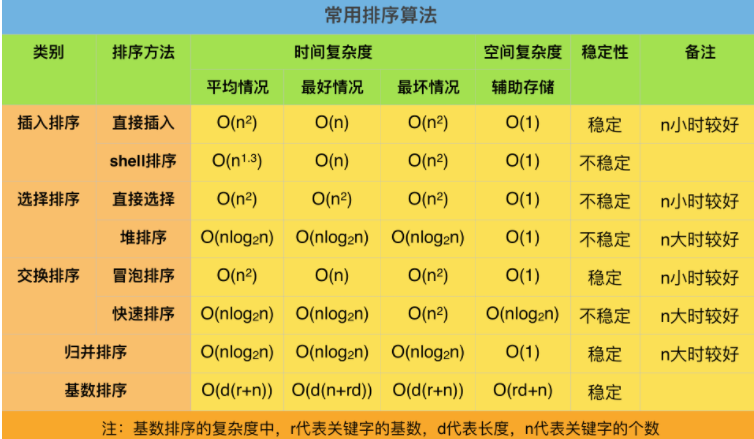
\includegraphics[width=.9\linewidth]{./pic/sort.png}

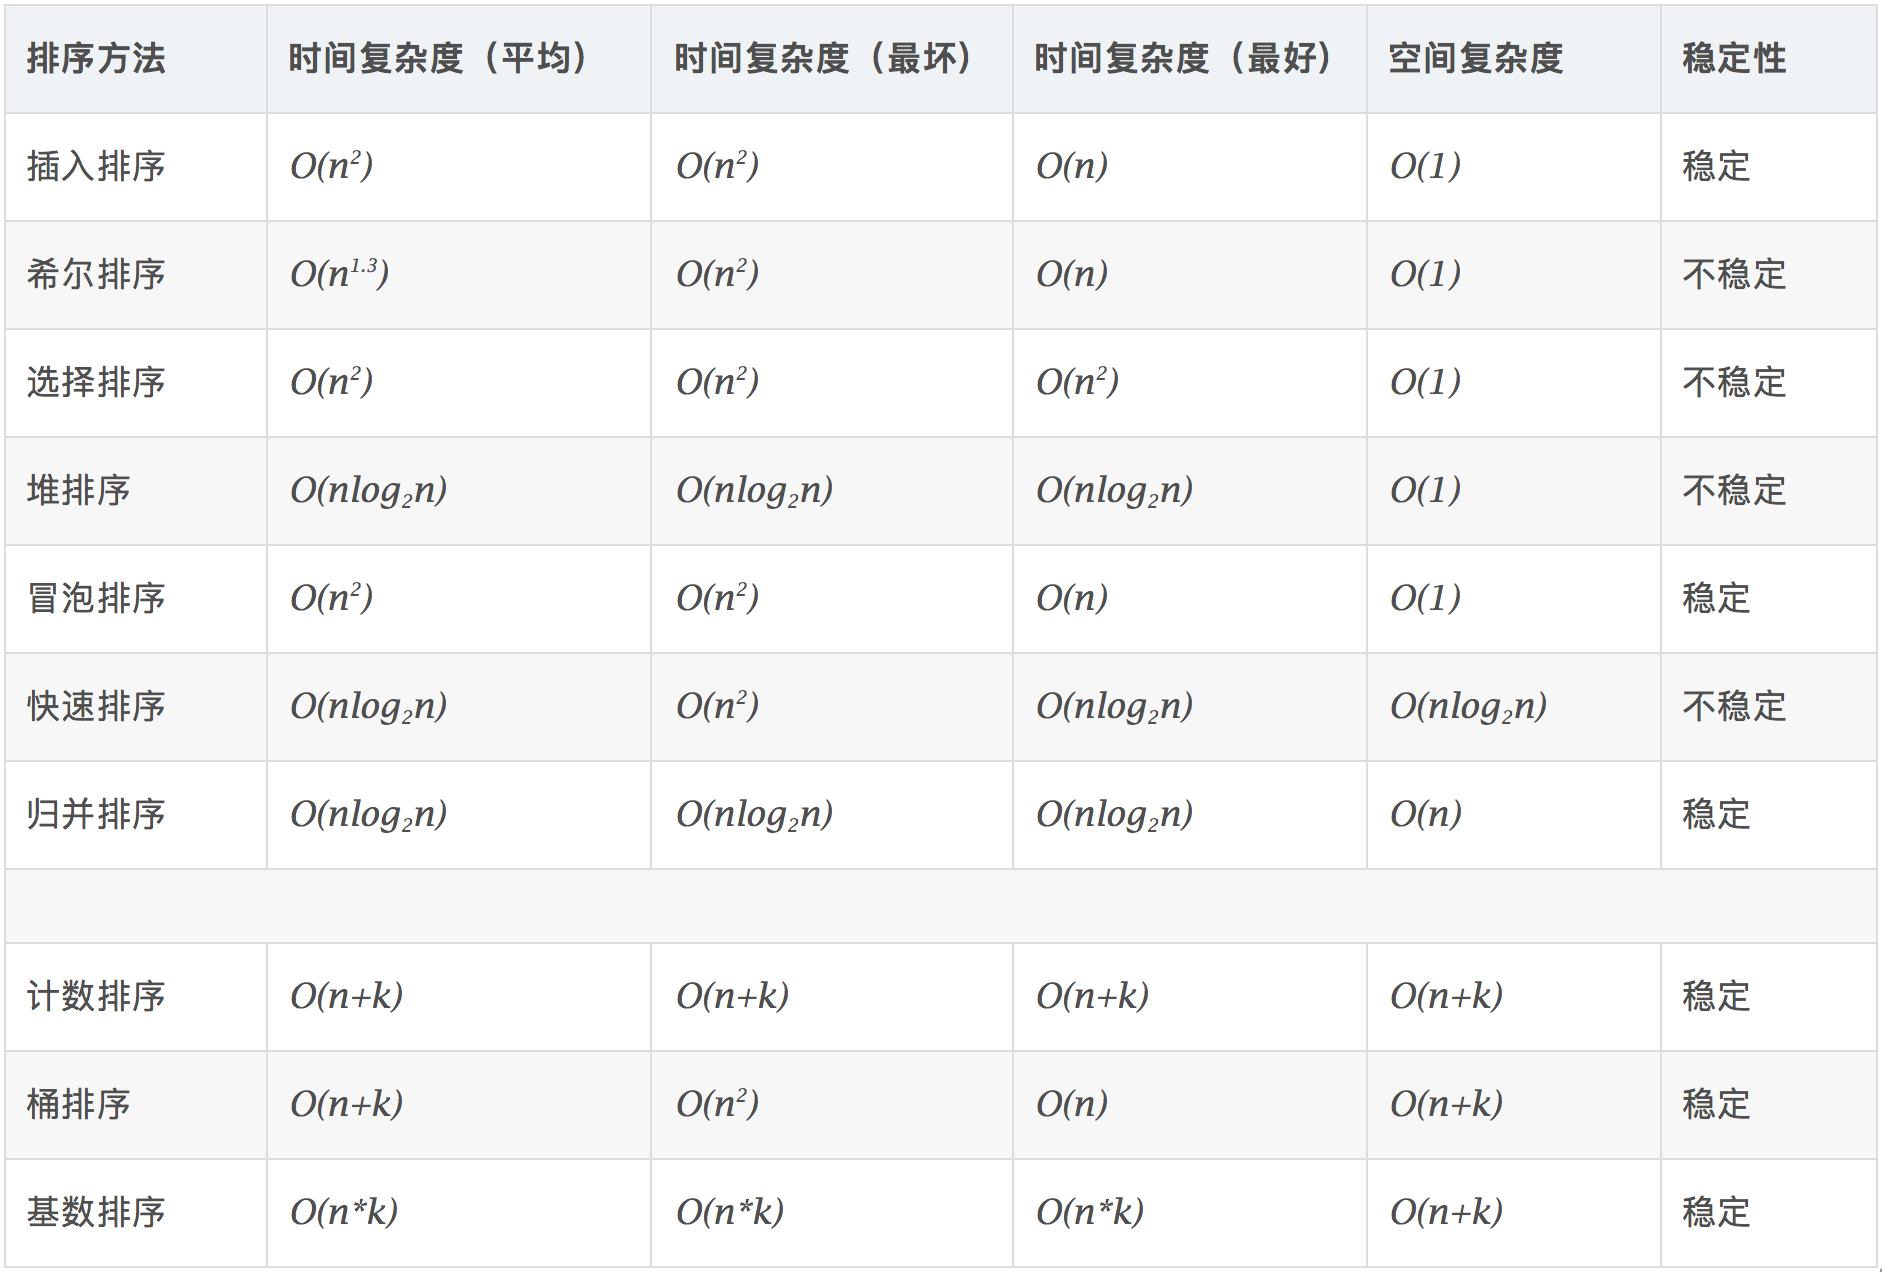
\includegraphics[width=.9\linewidth]{./pic/sort2.png}

\subsection{1996. The Number of Weak Characters in the Game 桶排序}
\label{sec-9-0-1}
You are playing a game that contains multiple characters, and each of the characters has two main properties: attack and defense. You are given a 2D integer array properties where properties[i] = [attacki, defensei] represents the properties of the ith character in the game.
A character is said to be weak if any other character has both attack and defense levels strictly greater than this character's attack and defense levels. More formally, a character i is said to be weak if there exists another character j where attackj > attacki and defensej > defensei.
Return the number of weak characters.
\begin{minted}[fontsize=\scriptsize,linenos=false]{csharp}
public int numberOfWeakCharacters(int[][] properties) {
    int maxAttrack = 0; // 找到所有士兵中的最大值
    for (int[] p : properties)
        maxAttrack = Math.max(maxAttrack,p[0]);
    // 为每一个攻击创建一个桶的位置
    int[] bucket = new int[maxAttrack + 2];     
    // 在每一个攻击力上找到最大的防御力
    for (int[] p : properties)
        bucket[p[0]] = Math.max(bucket[p[0]],p[1]);
    // 将桶的每一个位置都寻找到大于其攻击力的最大防御数值
    int rightMax = bucket[maxAttrack];
    for (int i = maxAttrack; i >= 0; i--) 
        if (rightMax > bucket[i])
            bucket[i] = rightMax;
        else
            rightMax = bucket[i];
    int ans = 0;
    // 最后遍历p 寻找所有的弱将
    for (int[] p : properties)
        if (bucket[p[0] + 1] > p[1]) ans++;  // 攻击力比当前小兵的攻击力大1的桶的位置存放着最大的防御力,与这个防御作比较可以得到当前小兵是否全面弱
    return ans;
}
public int numberOfWeakCharacters(int[][] properties) {
    int cnt = 0;
    int len = properties.length;
    Arrays.sort(properties, (a, b) -> (a[0] ! =  b[0] ? a[0]-b[0] : b[1]-a[1]));
    int max = properties[len-1][1];
    for(int i = len-1;i> = 0;i--){
        if(properties[i][1] < max)
            cnt++;
        max = Math.max(max,properties[i][1]);
    }
    return cnt;
}
\end{minted}

\subsection{Reverse Pairs}
\label{sec-9-0-2}
Given an integer array nums, return the number of reverse pairs in the array.
A reverse pair is a pair (i, j) where 0 <= i < j < nums.length and nums[i] > 2 * nums[j].
\begin{minted}[fontsize=\scriptsize,linenos=false]{csharp}
private int mergeSortCount(long [] arr, int bgn, int end) {
if (bgn >= end) return 0;
int mid = bgn + (end-bgn)/2;
int cnt = mergeSortCount(arr, bgn, mid) + mergeSortCount(arr, mid+1, end);
    for (int i = bgn, j = mid+1; i <= mid; i++) {
        while (j <= end && arr[i] > 2*arr[j]) j++;
        cnt += j - (mid+1);
    }
    Arrays.sort(arr, bgn, end+1);
    return cnt;
}
public int reversePairs(int[] nums) {
    int n = nums.length;
    return mergeSortCount(Arrays.stream(nums).mapToLong(i -> i).toArray(), 0, n-1);
}
// bit 的解法: https://www.cnblogs.com/grandyang/p/6657956.html
\end{minted}

\subsection{306. Additive Number}
\label{sec-9-0-3}
Additive number is a string whose digits can form additive sequence.

A valid additive sequence should contain at least three numbers. Except for the first two numbers, each subsequent number in the sequence must be the sum of the preceding two.

Given a string containing only digits '0'-'9', write a function to determine if it's an additive number.

Note: Numbers in the additive sequence cannot have leading zeros, so sequence 1, 2, 03 or 1, 02, 3 is invalid.
\begin{minted}[fontsize=\scriptsize,linenos=false]{csharp}
public boolean isAdditiveNumber(String num) {
    int n = num.length();
    if (n < 3) return false;
    for (int i = 1; i <= num.length() >> 1; i++)
        for (int j = 1; j + i < num.length(); j++)  
            if (isValid(num, num.substring(0, i), num.substring(i, i + j), i + j)) return true;
    return false;
}
private boolean isValid(String num, String first, String second, int index) {
    if (first.length() > 1 && first.startsWith("0") 
        || second.length() > 1 && second.startsWith("0")) return false;
    if (index == num.length()) return true; // 如果只有两个数是有效的!!!
    long sum = Long.parseLong(first) + Long.parseLong(second);
    if (num.startsWith(sum + "", index)) // 间接检测第三个数
        if (isValid(num, second, sum + "", index + (sum + "").length())) return true;
    return false;
}
\end{minted}


\chapter{Union Find 并查集}
\label{sec-10}
\subsection{1697. Checking Existence of Edge Length Limited Paths - Hard}
\label{sec-10-0-1}
An undirected graph of n nodes is defined by edgeList, where edgeList[i] = [ui, vi, disi] denotes an edge between nodes ui and vi with distance disi. Note that there may be multiple edges between two nodes.

Given an array queries, where queries[j] = [pj, qj, limitj], your task is to determine for each queries[j] whether there is a path between pj and qj such that each edge on the path has a distance strictly less than limitj .

Return a boolean array answer, where answer.length == queries.length and the jth value of answer is true if there is a path for queries[j] is true, and false otherwise.
\begin{enumerate}
\item 解题思路与分析: 离线排序优化
\label{sec-10-0-1-1}

我们可以分别对 edges 和 queries 进行一次升序排序。本题和 1170. 比较字符串最小字母出现频次 类似, 都可以采取 \textbf{离线排序优化} 的方式来解。

接下来,遍历 queries。遍历 queries 的同时将权值小于 limitj 的边进行合并。

接下来,我们只需要判断 pj 和 qj 是否已经在同一个联通域即可。

因此如果 pj 和 qj 在同一个联通域,那么其联通的路径上的所有边必定都小于 limitj,其原因就是前面加粗的那句话。

注意到排序打乱了 queries 的索引,因此我们需要记录一下其原始索引。

\begin{minted}[fontsize=\scriptsize,linenos=false]{csharp}
public boolean[] distanceLimitedPathsExist(int n, int[][] edgeList, int[][] queries) {
    DSU dsu = new DSU(n);
    Arrays.sort(edgeList, (a, b) -> a[2] - b[2]); // 同样按照weight的升序排列
    int m = queries.length, idx = 0, e = edgeList.length;
    Query [] qarr = new Query[m];
    for (int i = 0; i < m; i++) 
        qarr[i] = new Query(i, queries[i][0], queries[i][1], queries[i][2]);
    Arrays.sort(qarr);
    boolean [] ans = new boolean [m];
    for (int i = 0; i < m; i++) {
        while (idx < e && edgeList[idx][2] < qarr[i].weight) {
            dsu.union(edgeList[idx][0], edgeList[idx][1]);
            ++idx;
        }
        ans[qarr[i].idx] = dsu.areConnected(qarr[i].start, qarr[i].end);
    }            
    return ans;
}
private class DSU {
    private int N;
    private int [] parent, rank;
    public DSU( int n) {
        this.N = n;
        this.parent = new int [N];
        this.rank = new int [N];
        for (int i = 0; i < N; i++) {
            this.parent[i] = i;
            this.rank[i] = 1;
        }
    }
    public boolean areConnected(int u, int v) {
        return find(u) == find(v);
    }
    public void union(int u, int v) { // O(Log(N))
        if (u != v) {
            int p = find(u);
            int q = find(v);
            if (p != q) {
                if (rank[p] > rank[q]) {
                    parent[q] = p;
                    rank[p] += rank[q];
                } else {
                    parent[p] = q;
                    rank[q] += rank[p];
                }
            }
        }
    }
    private int find(int v) { 
        int x = v;
        while (x != parent[x])
            x = parent[x];
        parent[v] = x;
        return x;
    }
}
class Query implements Comparable<Query> {
    public int idx, start, end, weight;
    public Query(int idx, int bgn, int end, int weight) {
        this.idx = idx;
        this.start = bgn;
        this.end = end;
        this.weight = weight;
    }
    @Override public int compareTo(Query query) { // 按照weight的升序排列
        return this.weight - query.weight;
    }
}
// 令 m, q edges 和 queries 的长度。
//     时间复杂度:$O(mlogm + qlogq)
//     空间复杂度:$O(n + q)
// Runtime is bound by sorting: O(ElogE + NlogN + N + E);
\end{minted}
\end{enumerate}

\subsection{2003. Smallest Missing Genetic Value in Each Subtree - Hard}
\label{sec-10-0-2}
There is a family tree rooted at 0 consisting of n nodes numbered 0 to n - 1. You are given a 0-indexed integer array parents, where parents[i] is the parent for node i. Since node 0 is the root, parents\footnotemark[1]{} == -1.

There are 105 genetic values, each represented by an integer in the inclusive range [1, 105]. You are given a 0-indexed integer array nums, where nums[i] is a distinct genetic value for node i.

Return an array ans of length n where ans[i] is the smallest genetic value that is missing from the subtree rooted at node i.

The subtree rooted at a node x contains node x and all of its descendant nodes.
\begin{minted}[fontsize=\scriptsize,linenos=false]{csharp}
private void dfs(int i, Set<Integer> visited, int [] arr) { // 图的遍历:自顶向下ok,自底向上还不太熟悉,需要练习,还有一个没有消化好的类似题,找出来binary indexed tree
    if (!visited.contains(arr[i])) {
        Set<Integer> children = tree.getOrDefault(i, new HashSet<Integer>());
        for (int v : children) 
            dfs(v, visited, arr);
        visited.add(arr[i]);
    }
}
Map<Integer, Set<Integer>> tree = new HashMap<>();
int [] ans;
int n;
public int[] smallestMissingValueSubtree(int[] parents, int[] nums) {
    n = parents.length;
    ans = new int [n];
    Arrays.fill(ans, 1); 
    int oneIdx = -1;
    for (int i = 0; i < n; i++) 
        if (nums[i] == 1) {
            oneIdx = i;
            break;
        }
    if (oneIdx == -1) return ans;
    for (int i = 1; i < n; i++) {
        tree.computeIfAbsent(parents[i], k -> new HashSet<Integer>());
        tree.get(parents[i]).add(i);
        // tree.computeIfAbsent(i, k -> new HashSet<Integer>()); // 这里要想一下:为什么双向图他只加一个方向?
        // tree.get(i).add(parents[i]);
    }
    Set<Integer> visited = new HashSet<>(); // 这个直接转化为想要的结果,很便捷
    int parentIter = oneIdx;
    int miss = 1;
    while (parentIter >= 0) { // 从值为1的节点向根遍历(自底向上),没有任何重复计算,只走完这一条自底向项的路径就可以了
        dfs(parentIter, visited, nums);
        while (visited.contains(miss)) ++miss;
        ans[parentIter] = miss;
        parentIter = parents[parentIter];
    }
    return ans;
}
\end{minted}

\subsection{803. Bricks Falling When Hit - Hard 反向: 变de-Union vs为 Re-Union}
\label{sec-10-0-3}
You are given an m x n binary grid, where each 1 represents a brick and 0 represents an empty space. A brick is stable if:

It is directly connected to the top of the grid, or
At least one other brick in its four adjacent cells is stable.
You are also given an array hits, which is a sequence of erasures we want to apply. Each time we want to erase the brick at the location hits[i] = (rowi, coli). The brick on that location (if it exists) will disappear. Some other bricks may no longer be stable because of that erasure and will fall. Once a brick falls, it is immediately erased from the grid (i.e., it does not land on other stable bricks).

Return an array result, where each result[i] is the number of bricks that will fall after the ith erasure is applied.

Note that an erasure may refer to a location with no brick, and if it does, no bricks drop.


\includegraphics[width=.9\linewidth]{./pic/hitBricks.png}

\begin{minted}[fontsize=\scriptsize,linenos=false]{csharp}
private class UnionFind {
    int [] id; // parent
    int [] cnt;// size
    public UnionFind (int n) {
        id = new int [n];
        cnt = new int [n];
        for (int i = 0; i < n; i++) {
            id[i] = i;
            cnt[i] = 1;
        }
    }
    public int find(int i) {
        while (id[i] != i) {
            id[i] = id[id[i]];
            i = id[i];
        }
        return i;
    }
    public void union(int i, int j) {
        int rootI = find(i);
        int rootJ = find(j);
        if (rootI != rootJ) {
            id[rootI] = rootJ;
            cnt[rootJ] += cnt[rootI];
        }
    }
}
private void unionAround(int x, int y, int [][] arr, UnionFind uf) {
    for (int [] d : dirs) {
        int i = x + d[0];
        int j = y + d[1];
        if (i < 0 || i >= m || j < 0 || j >= n) continue;
        if (arr[i][j] == 1) uf.union(x*n+y+1, i*n+j+1); // +1
    }
    if (x == 0) uf.union(x*n+y+1, 0); // 第一排的直接与顶相连 // trick: to help calculate cnts connecting top easier/faster
}
int [][] dirs = {{1, 0}, {-1, 0}, {0, 1}, {0, -1}};
int m, n;
public int[] hitBricks(int[][] grid, int[][] hits) {
    m = grid.length;
    n = grid[0].length;
    for (int [] hit : hits)              // 首先把所有要打的砖块标记为2.
        if (grid[hit[0]][hit[1]] == 1)   // 如果有砖头
            grid[hit[0]][hit[1]] = 2;
    UnionFind uf = new UnionFind(m*n+1); // 这里的 + 1主要是多一个0来表示顶,所有的第一排的砖在unionfind的时候都会直接与这个0相连。
    for (int i = 0; i < m; i++)          // 然后对打掉后的数组中的砖块进行四个方向的union
        for (int j = 0; j < n; j++) 
            if (grid[i][j] == 1)
                unionAround(i, j, grid, uf);
    int cnt = uf.cnt[uf.find(0)];        // 这个count就是打完后一定会剩下的砖块数量.
    int [] ans = new int [hits.length];
    for (int i = hits.length-1; i >= 0; i--) {
        int [] hit = hits[i];
        if (grid[hit[0]][hit[1]] == 2) { // 对于需要复原的这个砖块做四个方向union,主要是为了得到有多少砖必须通过这块砖才能连接到顶部。
            unionAround(hit[0], hit[1], grid, uf);
            grid[hit[0]][hit[1]] = 1;    // 由于是从后向前,做完要把这块砖重新标记回来: 这些砖是有可能被hits前序砖敲掉后掉落下来的,不复原影响前序结果
        }
        int newCnt = uf.cnt[uf.find(0)];
        ans[i] = (newCnt - cnt > 0 ? newCnt - cnt - 1 : 0);
        cnt = newCnt;
    }
    return ans;
}
\end{minted}

\subsection{721. Accounts Merge}
\label{sec-10-0-4}
Given a list of accounts where each element accounts[i] is a list of strings, where the first element accounts[i]\footnotemark[1]{} is a name, and the rest of the elements are emails representing emails of the account.

Now, we would like to merge these accounts. Two accounts definitely belong to the same person if there is some common email to both accounts. Note that even if two accounts have the same name, they may belong to different people as people could have the same name. A person can have any number of accounts initially, but all of their accounts definitely have the same name.

After merging the accounts, return the accounts in the following format: the first element of each account is the name, and the rest of the elements are emails in sorted order. The accounts themselves can be returned in any order.

\begin{itemize}
\item Similar to the most voted solution, my solution uses the index of the owner as the key for the union map, to avoid possible issue caused by different owners have the same name, thus uses one less loop.
\end{itemize}

\begin{minted}[fontsize=\scriptsize,linenos=false]{csharp}
private int findParent(int [] arr, int x) {
    if (arr[x] == x) return x;
    arr[x] = findParent(arr, arr[x]);
    return arr[x];
}
public List<List<String>> accountsMerge(List<List<String>> accounts) {
    Map<String, Integer> owner = new HashMap<>();
    Map<Integer, TreeSet<String>> union = new HashMap<>(); // match idx & Set<Sting emails>
    int n = accounts.size(), p = 0;
    int [] par = new int [n];
    for (int i = 0; i < n; i++) par[i] = i;
    List<String> ls = new ArrayList<>(); 
    for (int i = 0; i < n; i++) { // find the ownerIdx for each email address
        ls = accounts.get(i);
        for (int j = 1; j < ls.size(); j++) {
            String email = ls.get(j);
            if (owner.containsKey(email)) {
                p = findParent(par, owner.get(email));
                par[p] = i; // union accounts that belong to the same user here by updating parent relation
            }
            owner.put(email, i);
        }
    }
     // union all emails belong to the same owner
    for (String emal : owner.keySet()) {
        int ownerIdx = findParent(par, owner.get(emal));
        TreeSet<String> set = union.getOrDefault(ownerIdx, new TreeSet<>());
        set.add(emal);
        union.put(ownerIdx, set);
    }
// Generate return result
    List<List<String>> res = new ArrayList<>();
    for (int ownerIdx : union.keySet()) {
        ls = new ArrayList<>();
        ls.add(accounts.get(ownerIdx).get(0));  // get the owner name
        ls.addAll(union.get(ownerIdx));
        res.add(ls);
    }
    return res;
}
\end{minted}

\subsection{1202. Smallest String With Swaps}
\label{sec-10-0-5}
You are given a string s, and an array of pairs of indices in the string pairs where pairs[i] = [a, b] indicates 2 indices(0-indexed) of the string.

You can swap the characters at any pair of indices in the given pairs any number of times.

Return the lexicographically smallest string that s can be changed to after using the swaps.
\begin{minted}[fontsize=\scriptsize,linenos=false]{csharp}
int [] par;
int [] rank;
int n;
public int find(int v) {
    if (v != par[v] ) 
        par[v] = find(par[v]);
    return par[v];
}
public boolean union(int i, int j) {
    int ri = find(i);
    int rj = find(j);
    if (ri == rj) return false;
    if (rank[ri] < rank[rj]) par[ri] = rj;
    else if (rank[ri] > rank[rj]) par[rj] = ri;
    else {
        par[rj] = ri;
        rank[ri] ++; // 维护rank的值
    }
    return true;
}
public String smallestStringWithSwaps(String s, List<List<Integer>> pairs) {
    int n = s.length();
    par = new int [n];
    rank = new int [n];
    List<Queue<Character>> list = new ArrayList<>(n);
    for (int i = 0; i < n; i++) {
        par[i] = i;
        list.add(new PriorityQueue<>());
    }
    Arrays.fill(rank, 1);
    pairs.forEach(p -> union(p.get(0), p.get(1))); // Perform union for each pair.
    // Add each character to the priority queue associated with its component.
    IntStream.range(0, n).forEach(index -> list.get(find(index)).add(s.charAt(index)));
    // Build the result, by removing chars from the corresponding priority queue.
    StringBuilder buffer = new StringBuilder(n);
    IntStream.range(0, n).forEachOrdered(index -> buffer.append(list.get(find(index)).remove()));
    return buffer.toString();
}
// O(NlogN). Worst-case, all indices are part of the same component. So we will essentially be popping off from the same priority queue.
// Space Complexity: O(N).
\end{minted}

\subsection{1998. GCD Sort of an Array - Hard}
\label{sec-10-0-6}
You are given an integer array nums, and you can perform the following operation any number of times on nums:

Swap the positions of two elements nums[i] and nums[j] if gcd(nums[i], nums[j]) > 1 where gcd(nums[i], nums[j]) is the greatest common divisor of nums[i] and nums[j].
Return true if it is possible to sort nums in non-decreasing order using the above swap method, or false otherwise.
\begin{minted}[fontsize=\scriptsize,linenos=false]{csharp}
private int find (int v) {
    if (!parent.containsKey(v)) {
        parent.put(v, v);
        return v;
    }
    if (parent.get(v) != v)
        parent.put(v, find(parent.get(v)));
    return parent.get(v);
}
private void union(int x, int y) {
    int rx = find(x);
    int ry = find(y);
    if (rx != ry) parent.put(rx, ry);
}
/**
   general idea (not accepted)
   we can simply union pairs of numbers which has gcd > 1 in quadratic time and then check of groups that
   are formed by union of pairs can be invidually sorted. 
   improved (accpeted)
   In above approach problem is we are union-ing pairs in quadratic time. To improve upon it. We union a number
   which is present in 'nums' with its smallest prime factor. thus if two numbers has same smallest prime factor
   their gcd is guaranted to be > 1. 
**/
Map<Integer, Integer> parent = new HashMap<>();
public boolean gcdSort(int[] arr) {
    int n = arr.length;
    parent = new HashMap<Integer, Integer>();
    int [] sorted = arr.clone();
    Arrays.sort(sorted);
    int max = Arrays.stream(arr).max().getAsInt();
    Set<Integer> numSet = new HashSet<>();
    numSet.addAll(Arrays.stream(arr).boxed().collect(Collectors.toList()));
    int p = 2;  // Seive algorithm
    boolean [] primes = new boolean [max + 1];
    Arrays.fill(primes, true);
    while (p < max) {
        if (primes[p]) {
            for (int i = p; i <= max; i += p) { // 我合并的是数组的索引,他优化成合并所有拥有公约数为p的数组中沿未合并的值
                if (numSet.contains(i)) union(p, i);
                primes[i] = false;
            }
        }
        p++;
    }
    for (int i = 0; i < n; i++) 
        if (arr[i] != sorted[i] && find(sorted[i]) != find(arr[i])) return false;
    return true;
}
\end{minted}

\subsection{1724 给定一个n nn个顶点的无向带权图,要求在线回答若干询问,每次询问是个三元组( p , q , x ) (p,q,x)(p,q,x),是问是否存在p pp到q qq的每条边都小于x xx的路径。}
\label{sec-10-0-7}

先以Kruskal算法求最小生成森林,显然对于任何p pp和q qq,它们之间所有路径中最大边最小的那条路径的最大边一定是最小生成树的某条边(如果存在路径的话)。建树完成之后,对每个连通块,以任意顶点为根,将该连通块做成一棵有根树。对于每次询问,我们只需求p pp和q qq所有到它们的最近公共祖先所经过的边的最大边权就行了。可以考虑用倍增思想(以下的内容可以参考\url{https://blog.csdn.net/qq_46105170/article/details/116217633),开两个数组f} ff和g gg,其中f [ i ] [ k ] f[i][k]f[i][k]指的是从i ii节点向上跳2 k 2\^{}k2 
k
 步能过走到的顶点是谁(如果跳出界了则规定值为− 1 -1−1),g [ i ] [ k ] g[i][k]g[i][k]指的是从i ii节点向上跳2 k 2\^{}k2 
k
 的过程中经过的边的最大权值(在不会跳出界的情况下),然后从每个树根做BFS,初始化f [ . ] [ 0 ] f[.]\footnotemark[1]{}f[.]\footnotemark[1]{}和g [ . ] [ 0 ] g[.]\footnotemark[1]{}g[.]\footnotemark[1]{}。由于在询问的时候需要知道最近公共祖先,所以还需要一个数组d dd记录每个顶点的深度,在BFS的时候可以同时求出。接下来,用倍增的思想计算f ff和g gg:
\begin{minted}[fontsize=\scriptsize,linenos=false]{csharp}
f[i][k] = f[f[i][k-1]][k-1]
g[i][k] = max{g[i][k-1],g[f[i][k-1]][k-1]}
\end{minted}
至此,所有的预处理就完成了。

接下来询问的时候,如果p pp与q qq不连通则直接返回false。否则看一下两个顶点的深度,不妨设p pp更深,则将p pp向上跳若干步,使得p pp与q qq一样深,同时用经过的边权更新答案。此时如果p = q p=qp=q,则答案已经求出,与x xx比较即可;否则,将p pp与q qq继续向上跳,一路跳到它们的最近公共祖先的孩子的那层位置,一路更新答案,最后再用最近公共祖先与它们的连边更新答案,最后将答案与x xx比较。代码如下:
\begin{minted}[fontsize=\scriptsize,linenos=false]{csharp}
public class DistanceLimitedPathsExist {
    class UnionFind {
        private int[] p;
        public UnionFind(int size) {
            p = new int[size];
            for (int i = 0; i < size; i++) 
                p[i] = i;
        }
        public int find(int x) {
            if (p[x] != x) 
                p[x] = find(p[x]);
            return p[x];
        }
        public void union(int x, int y) {
            int px = find(x), py = find(y);
            if (px != py) 
                p[px] = py;
        }
    }
    private UnionFind uf;
    // 这里是链式前向星建图
    private int[] h, e, ne, w;
    private int idx;
    private void add(int a, int b, int c) {
        e[idx] = b;
        ne[idx] = h[a];
        w[idx] = c;
        h[a] = idx++;
    }
    // 这里是倍增法所需的数组和变量
    private int[][] f, g;
    private int[] depth;
    // n是顶点数,log是n对2的对数,log + 1也是f的第二维应该开的长度
    private int n, log;
    public DistanceLimitedPathsExist(int n, int[][] edgeList) {
        this.n = n;
        depth = new int[n];
        h = new int[n];
        Arrays.fill(h, -1);
        // 无向图,边要开两倍
        e = new int[n << 1];
        ne = new int[n << 1];
        w = new int[n << 1];
        // 这一段是Kruskal算法建最小生成森林
        Arrays.sort(edgeList, (e1, e2) -> Integer.compare(e1[2], e2[2]));
        uf = new UnionFind(n);
        for (int[] e : edgeList) {
            int a = e[0], b = e[1], len = e[2];
            if (uf.find(a) != uf.find(b)) {
                uf.union(a, b);
                add(a, b, len);
                add(b, a, len);
            }
        }
        log = (int) (Math.log(n) / Math.log(2));
        f = new int[n][log + 1];
        g = new int[n][log + 1];
        for (int[] row : f) {
            Arrays.fill(row, -1);
        }
        boolean[] vis = new boolean[n];
        for (int i = 0; i < n; i++) {
            if (!vis[i]) {
                bfs(i, vis);
            }
        }
        init();
    }
    // 递推一遍f和g数组
    private void init() {
        for (int i = 1; i < log + 1; i++) {
            for (int j = 0; j < n; j++) {
                if (f[j][i - 1] != -1) {
                    f[j][i] = f[f[j][i - 1]][i - 1];
                    g[j][i] = Math.max(g[j][i - 1], g[f[j][i - 1]][i - 1]);
                }
            }
        }
    }
    // BFS一遍x所在连通块,并初始化f和g数组,并求出depth数组
    private void bfs(int x, boolean[] vis) {
        Queue<Integer> q = new ArrayDeque<>();
        q.offer(x);
        vis[x] = true;
        while (!q.isEmpty()) {
            int u = q.poll();
            for (int i = h[u]; i != -1; i = ne[i]) {
                int v = e[i];
                if (vis[v]) continue;
                vis[v] = true;
                f[v][0] = u;
                g[v][0] = w[i];
                q.offer(v);
                depth[v] = depth[u] + 1;
            }
        }
    }
    public boolean query(int p, int q, int limit) {
        if (uf.find(p) != uf.find(q)) 
            return false;
        if (depth[p] < depth[q]) {
            int tmp = p;
            p = q;
            q = tmp;
        }
        // 先走到同一深度
        int diff = depth[p] - depth[q];
        int pow = 0, max = 0;
        while (diff > 0) {
            if ((diff & 1) == 1) {
                max = Math.max(max, g[p][pow]);
                p = f[p][pow];
            }

            pow++;
            diff >>= 1;
        }
        // 已经走到同一点了,那深度更浅的那个点就是最近公共祖先,max就是经过的边的最大值
        if (p == q) return max < limit;
        // 否则跳到最近公共祖先下面一层,沿途更新答案
        for (int i = log; i >= 0; i--) {
            if (f[p][i] != f[q][i]) {
                max = Math.max(max, g[p][i]);
                max = Math.max(max, g[q][i]);
                p = f[p][i];
                q = f[q][i];
            }
        }
        // 最后别忘了用最后一步更新答案
        max = Math.max(max, g[p][0]);
        max = Math.max(max, g[q][0]);
        return max < limit;
    }
}
// 初始化时间复杂度O ( m log ⁡ m + n log ⁡ n ) O(m\log m+n\log n)O(mlogm+nlogn),每次询问时间O ( log ⁡ n ) O(\log n)O(logn),空间O ( m + n + n log ⁡ n ) O(m+n+n\log n)O(m+n+nlogn)。
\end{minted}

\subsection{1172. 祖孙询问}
\label{sec-10-0-8}
给定一棵包含n nn个节点的有根无向树,节点编号互不相同,但不一定是1 ∼ n 1∼n1∼n。有m mm个询问,每个询问给出了一对节点的编号x xx和y yy,询问x xx与y yy的祖孙关系。

输入格式:
输入第一行包括一个整数 表示节点个数;接下来n nn行每行一对整数a aa和b bb,表示a aa和b bb之间有一条无向边。如果b bb是− 1 −1−1,那么a aa就是树的根;第n + 2 n+2n+2行是一个整数m mm表示询问个数;接下来m mm行,每行两个不同的正整数x xx和y yy,表示一个询问。

输出格式:
对于每一个询问,若x xx是y yy的祖先则输出1 11,若y yy是x xx的祖先则输出2 22,否则输出0 00。

数据范围:
1 ≤ n , m ≤ 4 × 1 0 4 1≤n,m≤4×10\^{}41≤n,m≤4×10 
4

1 ≤ v ≤ 4 × 1 0 4 1≤v≤4×10\^{}41≤v≤4×10 
4
 ,v vv是顶点编号

可以用倍增的思想来求。预处理两个数组,一个是d [ i ] d[i]d[i],指的是顶点i ii的深度,树根深度是1 11,其余顶点的深度就是其与树根的路径边数;另一个是f [ i ] [ k ] f[i][k]f[i][k],是从顶点i ii向树根方向(以下均称“向上”)跳2 k 2\^{}k2 
k
 步走到的顶点。由于顶点编号都是大于0 00的,我们可以人为规定一个0 00号节点作为哨兵,并且∀ k , f [ r ] [ k ] = 0 $\forall$ k,f[r][k]=0∀k,f[r][k]=0,d [ 0 ] = 0 d\footnotemark[1]{}=0d\footnotemark[1]{}=0,其中r rr是树根编号。这样如果k kk太大导致跳出树根的话,就会得到跳到了哨兵的结论。那么对于f ff,有f [ i ] [ 0 ] = p i f[i]\footnotemark[1]{}=p\_if[i]$\backslash$footnotemark[1]\{\}= 是i ii的父亲,并且:

f[i][k]=f[f[i][k−1]][k−1]

即分两次跳,一次跳2\^{}k 步等价于两次跳2\^{}k-1 步。初始化f ff和d dd数组的过程,可以用一次从树根的BFS来做到。

在询问的时候,比如询问a aa和b bb的公共祖先,不妨设a aa的深度更深,那么先让a aa向上跳到与b bb深度相同,可以先计算一下d [ a ] − d [ b ] d[a]-d[b]d[a]−d[b],然后将这个数字做二进制分解,就可以由f ff数组算出从a aa向上走到与b bb深度相同的时候是哪个顶点;接着再从a aa和b bb一起向上走,直到走到它们真正的最近公共祖先的下一层为止(即跳的步数是当前深度差减1 11),此时f [ a ] [ 0 ] f[a]\footnotemark[1]{}f[a]\footnotemark[1]{}即为最近公共祖先。代码如下:
\begin{minted}[fontsize=\scriptsize,linenos=false]{c++}
const int N = 40010, M = N * 2;
int n, m;
int h[N], e[M], ne[M], idx;
int depth[N], fa[N][16];
int q[N];
void add(int a, int b) {
    e[idx] = b, ne[idx] = h[a], h[a] = idx++;
}
// 从树根开始bfs,预处理出d数组和f数组
void bfs(int root) {
    memset(depth, 0x3f, sizeof depth);
    depth[0] = 0, depth[root] = 1;
    int hh = 0, tt = 0;
    q[tt++] = root;
    while (hh < tt) {
        int t = q[hh++];
        for (int i = h[t]; ~i; i = ne[i]) {
            int j = e[i];
            if (depth[j] > depth[t] + 1) {
                depth[j] = depth[t] + 1;
                q[tt++] = j;
                // 预处理f数组
                fa[j][0] = t;
                for (int k = 1; k <= 15; k++) 
                    fa[j][k] = fa[fa[j][k - 1]][k - 1];
            }
        }
    }
}
int lca(int a, int b) {
	// 强制让a的深度大于等于b的深度
    if (depth[a] < depth[b]) swap(a, b);
    // 从大到小枚举k,将a向上跳到与b同层
    for (int k = 15; k >= 0; k--)
        if (depth[fa[a][k]] >= depth[b]) 
            a = fa[a][k];
	// 如果a和b重合了,那么说明b就是最近公共祖先
    if (a == b) return b;
    // 否则将a和b同时向上跳,直到跳到最近公共祖先下一层为止
    for (int k = 15; k >= 0; k--)
        if (fa[a][k] != fa[b][k])
            a = fa[a][k], b = fa[b][k];
    return fa[a][0];
}
int main() {
    scanf("%d", &n);
    memset(h, -1, sizeof h);
    int root = 0;
    for (int i = 0; i < n; i++) {
        int a, b;
        scanf("%d%d", &a, &b);
        if (b == -1) root = a;
        else add(a, b), add(b, a);
    }
    bfs(root);
    scanf("%d", &m);
    while (m--) {
        int a, b;
        scanf("%d%d", &a, &b);
        int p = lca(a, b);
        if (p == a) puts("1");
        else if (p == b) puts("2");
        else puts("0");
    }
    return 0;
}
\end{minted}

\subsection{某个网友列的相关题目: 并查集参考:数据结构–并查集(Disjoint-Set)}
\label{sec-10-0-9}
\begin{itemize}
\item 261. 以图判树(全部连通+边数=V-1)
\item 305. 岛屿数量 II(并查集)
\item 323. 无向图中连通分量的数目(并查集)
\item 684. 冗余连接(并查集)
\item 685. 冗余连接 II(并查集)
\item 721. 账户合并(并查集)(字符串合并)
\item 737. 句子相似性 II(并查集)
\item 886. 可能的二分法(着色DFS/BFS/拓展并查集)
\item 947. 移除最多的同行或同列石头(并查集)
\item 990. 等式方程的可满足性(并查集)
\item 959. 由斜杠划分区域(并查集)
\item 1061. 按字典序排列最小的等效字符串(并查集)
\item 1101. 彼此熟识的最早时间(排序+并查集)
\item 1202. 交换字符串中的元素(并查集)
\item 1319. 连通网络的操作次数(BFS/DFS/并查集)
\item 5510. 保证图可完全遍历(并查集)
\item 程序员面试金典 - 面试题 17.07. 婴儿名字(并查集)
\end{itemize}
% Emacs 28.2 (Org mode 8.2.7c)
\end{document}